\documentclass[12pt]{article}
\usepackage[left=1in,right=1in,top=1in,bottom=1in]{geometry}                % See geometry.pdf to learn the layout options. There are lots.
\geometry{letterpaper} 
\usepackage{appendix}
\usepackage{pgflibraryarrows}
\usepackage{pgflibrarysnakes}
\usepackage{pgfplots}
\pgfplotsset{compat=newest}
\usetikzlibrary{patterns}
\usepackage{xcolor}
\usepackage{mathpazo}
\usepackage{graphicx}
\usepackage{amssymb}
\usepackage{mathrsfs}
\usepackage{standalone}
\usepackage{epstopdf}
\DeclareGraphicsRule{.tif}{png}{.png}{`convert #1 `dirname #1`/`basename #1 .tif`.png}

\usepackage{float}
\usepackage{rotfloat}
\usepackage{booktabs}
% \usepackage{graphicx} % already loaded above
\usepackage{setspace}
\onehalfspacing
% \doublespacing
\usepackage[authoryear]{natbib}
\usepackage{threeparttable}
\usepackage{tabularx}
\usepackage{comment}
\usepackage{subcaption}
\usepackage{wrapfig}
\usepackage{adjustbox}
\usepackage{bbm}
\usepackage{dsfont} % provides \mathds{1} used in demand and summary tables
\usepackage{enumitem}
% \usepackage{pgfplots} % already loaded above
% \pgfplotsset{compat=1.8} % overrides earlier compat=newest setting
\usepackage{mathtools}
\usepackage{amsfonts}
\usepackage{multicol}
\usepackage{amsthm}
% \usepackage{graphics} % superseded by graphicx, loaded above
\usepackage{amsmath}
\usepackage{amsxtra}
\usepackage{amstext}
\usepackage{latexsym}
% \usepackage[authoryear]{natbib} % already loaded above
\usepackage[pdftex,bookmarks=true,bookmarksopen=true,pdfpagemode=UseOutlines,pdfstartview=FitH]{hyperref}
\usepackage{indentfirst}
\usepackage{tikz}
\usetikzlibrary{intersections,positioning,calc}
\usetikzlibrary {arrows.meta,bending,positioning}
\usetikzlibrary{decorations.pathreplacing,calligraphy}
%\usepackage{pgflibraryarrows}
%\usepackage{pgflibrarysnakes}
\usepackage{longtable}
% \usepackage{threeparttable} % already loaded above
% \usepackage{tabularx} % already loaded above
\usepackage{pdflscape}
\usepackage{afterpage}
%\usepackage{fourier} % font: utopia
\let\counterwithout\relax
\let\counterwithin\relax
\usepackage{chngcntr}
% \usepackage{hyperref} % already loaded above
\hypersetup{hidelinks}
\usepackage{array}
\usepackage[utf8]{inputenc}
\usepackage{fancyvrb}
\usepackage{fancyhdr}
\usepackage{placeins}
\newcolumntype{H}{>{\setbox0=\hbox\bgroup}c<{\egroup}@{}}
\linespread{1.3}
\usepackage{bm}
\newcommand{\bs}{\boldsymbol}
% \sym is used for significance stars in the demand and first-stage tables
% (estout-style). Defined here so the document compiles.
\providecommand{\sym}[1]{\ensuremath{^{#1}}}
\usetikzlibrary{calendar,shapes.geometric,backgrounds,positioning}
\usepackage{nicefrac}

% Unused citation aliases from a prior template (CMS/AHA — not cited in this paper).
% Kept commented in case they are needed later.
% \defcitealias{CMSLandscape}{CMS, 2021a}
% \defcitealias{CMSRatebooks}{CMS, 2021b}
% \defcitealias{EnrollmentCPSC}{CMS, 2021c}
% \defcitealias{StarRatings}{CMS, 2021d}
% \defcitealias{BidPricingTool}{CMS, 2022a}
% \defcitealias{GeographicPUF}{CMS, 2022b}
% \defcitealias{AHRFphysiciandensity}{AHRF, 2021}
% \defcitealias{AHAhospitalHHI}{AHA, 2016}


% \usepackage{tikz} % already loaded above
% \usetikzlibrary{positioning} % already loaded above

\interfootnotelinepenalty=10000


\begin{document}


%\title{Learning-by-Doing, Industrial Policies, and Technological Adoption: Evidence from China's Solar Panel Industry}
\title{Learning-by-Doing, Industrial Policy, and the Rise of Crystalline Silicon Solar Panels\footnote{We thank Gang He and conference and seminar participants for helpful comments. All errors are our own.}}
\author{Dana Golden \and Xiangjun Ma \and  Yiyi Zhou\thanks{Golden: Department of Economics, Stony Brook University, dana.golden@stonybrook.edu. Ma: School of Finance and Trade, Liaoning University, aqj474@gmail.com. Zhou: Department of Economics, Stony Brook University, yiyi.zhou@stonybrook.edu.}}



\maketitle

\begin{abstract}

\singlespacing 

%Crystalline silicon (c-Si) technology has dominated in the solar panel manufacturing and the production costs have declined by \textcolor{blue}{XX\%} over the past decade. This study investigates the role of learning-by-doing (LBD) in driving this cost reduction and forming the technological pathway of the industry, and its interaction with input price and government subsidy policies.

This paper studies how learning-by-doing shapes cost dynamics, technological adoption, and the effectiveness of industrial policies in the solar panel industry. We develop and estimate a dynamic model of firm entry, exit, production, and technology choice using firm-level data on Chinese manufacturers and global data from 2000 to 2013. The model allows production experience to reduce future costs, generating a dynamic feedback loop between output and productivity.
% TODO(units): Section 5 reports the LBD magnitude as ``per MW'' (e.g., \$0.708/MW for a typical c-Si firm). If marginal costs are denominated per Watt elsewhere in the paper, verify the unit before submission and update the abstract/intro accordingly.
We find that learning-by-doing is a key driver of cost reductions, particularly for crystalline silicon (c-Si) technology: doubling cumulative production reduces marginal costs by approximately \$0.71 per MW for a typical c-Si firm and \$1.82 per MW for large c-Si firms. Learning also amplifies the effects of industrial policies, leading to larger long-run impacts on output and prices. It further shapes technological competition, contributing to the dominance of c-Si technology. Finally, earlier policy implementation yields substantially larger effects by accelerating movement along the experience curve.

\thispagestyle{empty}

\begin{description}
\item[Keywords:] learning-by-doing, industrial policy, technological path dependence, solar panels 

\item[JEL Classification Codes:] % TODO(JEL): confirm/edit. Suggested based on content: L52 (industrial policy), L94 (electric utilities), O33 (technological change: choices and consequences), Q42 (alternative energy sources), Q48 (energy: government policy), F13 (trade policy).
L52, L94, O33, Q42, Q48, F13
\end{description}
\end{abstract}

%\newpage\tableofcontents

\clearpage
\setcounter{page}{1}

\section{Introduction}

The development of solar energy plays a crucial role in the transition to a sustainable and low-carbon electricity grid and the mitigation of climate change. The rapid decline in the cost of solar panels over the past two decades has been one of the most striking developments in energy markets. At the same time, the industry has experienced a dramatic shift in its technological composition, with crystalline silicon (c-Si) emerging as the dominant technology worldwide. Understanding the forces driving these changes is central to evaluating the effectiveness of industrial policies and the transition to low-carbon energy systems.

A large body of work has attributed the decline in solar panel costs to learning-by-doing (LBD), whereby cumulative production experience reduces future production costs. During the same period, governments around the world implemented a wide range of industrial policies, including demand-side subsidies, supply-side subsidies, and trade policies. %In addition, key input prices—most notably polysilicon, the primary input for c-Si panels—experienced substantial fluctuations. 
While each of these factors has been studied in isolation, less is known about how they interact to shape industry dynamics.

This paper studies how learning-by-doing interacts with industrial policies to determine production costs, technology adoption, and welfare in the solar panel industry. We focus on a central mechanism: policies affect production not only directly, but also indirectly through their impact on cumulative experience. This generates a dynamic feedback loop in which higher output today lowers future costs, further increasing output and accelerating the adoption of particular technologies.

To quantify this mechanism, we develop and estimate a dynamic model of firm behavior in the global solar panel industry. The model incorporates firm entry and exit, technology choice, and production decisions, allowing firms’ costs to evolve endogenously with cumulative production. We estimate the model using a combination of firm-level data on Chinese manufacturers and aggregate data on global prices, input costs, and policy variables from 2000 to 2013.

Our empirical analysis yields three main findings.
First, learning-by-doing is a quantitatively important driver of cost reductions, particularly for c-Si technology. We estimate that doubling cumulative production reduces marginal costs by approximately \$0.71 per MW for a typical c-Si firm (and \$1.82 per MW for large c-Si firms), implying that LBD accounts for a substantial share of the observed decline in solar panel prices.
Second, learning-by-doing significantly amplifies the effects of industrial policies. For example, the decline in polysilicon prices not only reduces costs directly, but also increases production, which accelerates learning and further reduces costs. Similarly, demand-side subsidies and entry subsidies generate larger long-run effects when learning is present than when it is absent. Ignoring LBD would therefore lead to a substantial underestimation of the impact of these policies.
Third, learning-by-doing plays a key role in shaping technological competition. Because c-Si technology exhibits stronger learning effects than thin-film technology, policies and shocks that expand production disproportionately benefit c-Si, contributing to its eventual dominance.

We further show that the timing of policies is critical. Demand-side subsidies are significantly more effective when implemented early, as they initiate the learning process and generate persistent cost reductions. Similarly, supply-side policies yield larger benefits when introduced earlier, as they accelerate movement along the experience curve. These results highlight the importance of accounting for dynamic complementarities when designing industrial policies.

This paper contributes to several strands of literature. First, it contributes to the literature on industrial policies in renewable energy markets. Many of these studies, including \citet{de2019subsidies}, focus on the impact of demand-side subsidies. One exception is
\citet{bollinger2025strategic}, who examines how import tariffs affect market equilibrium outcomes and compares import tariffs to supply-side subsidies. To the best of our knowledge, our study is the first to jointly analyze demand-side and supply-side interventions within a unified framework. 

Second, it adds to the empirical literature on learning-by-doing that has been documented in a variety of industries, for example, \citet{head1994infant} and \citet{ohashi2005learning} on steel, \citet{thompson2001much} and \citet{thornton2001learning} on shipbuilding, \citet{benkard2000learning} and \citet{benkard2004dynamic} on aircraft, \citet{su2025LBD} on space launch.  %Almost all previous studies relied on data on input requirements or costs associated with producing a product, but these data are often hard to obtain for researchers. Exceptions include \citet{covert2022winds} and \citet{barwick2025drive}. 
In particular, our paper contributes to the growing literature studying learning-by-doing in low-carbon technology sectors. For example, \citet{helveston2022quantifying} estimates a two-factor learning model and finds the learning rates of solar panel module production in Germany, U.S., and China are 20\%, 26\%, and 33\% between 2006 to 2020, respectively. \citet{barwick2025drive} estimates a static model where electric vehicle producers and battery producers bargain over prices and finds a sizable LBD of battery production. 
Our approach is in the same spirit of theirs by exploiting variations in prices and quantities of the final products and main inputs. We quantify its role in a setting with rich firm-level data and multiple interacting policy instruments. 

%In particular, our paper contributes to the growing literature studying learning-by-doing in low-carbon technology sectors, such as solar panel, wind generating systems, and electric vehicles.  \citet{barwick2025drive} ... \citet{helveston2022quantifying} estimates a two-factor learning model using the annual installed capacities and prices of solar panel modules in Germany, U.S., and China between 2006 to 2020 and finds that the learning rates are 20\%, 26\%, and 33\% in these three countries, respectively.

Our paper also contributes to the literature on technological path dependence and technological competition. A central insight of this literature is that small initial advantages—arising from costs, policies, or shocks—can be amplified over time, leading to the dominance of one technology even in the presence of viable alternatives. In our setting, learning-by-doing provides a concrete mechanism for such path dependence. Because cumulative production reduces future costs, technologies that experience early expansion—whether due to input price declines or policy support—become progressively more competitive, reinforcing their adoption over time. We show that this dynamic feedback loop helps explain the rapid diffusion and eventual dominance of crystalline silicon technology over thin-film alternatives. By quantifying how policies and input price shocks interact with learning-by-doing, our analysis provides new empirical evidence on how technological pathways are shaped in dynamic industries and highlights the role of policy timing in influencing long-run technological outcomes.

More broadly, our findings suggest that evaluating industrial policies in emerging industries requires accounting for dynamic production externalities such as learning-by-doing. Policies that stimulate early production can have long-lasting effects by shaping the trajectory of costs and technology adoption, while delayed interventions may forgo these dynamic gains.

The remainder of the chapter proceeds as follows. Section~\ref{sec:institution_data} describes the solar panel industry and the data. Section~\ref{sec:LBDmodel} presents the model. Section~\ref{sec:LBDestimation} outlines the estimation strategy. Section~\ref{sec:LBDresults} reports the estimation results. Section~\ref{sec:LBDcounterfactuals} presents the counterfactual analysis. Section~\ref{sec:LBDconclusion} concludes.




\section{Solar Panel Industry and Data}
\label{sec:institution_data}

\subsection{Technologies of Solar Panel Manufacturing}
\label{subsec:inst_PV_tech}
Over the past three decades, two primary technologies have been used to manufacture solar panels: crystalline silicon (c-Si) and thin-film technologies.

Crystalline silicon technology, first developed at Bell Labs in 1954, has become the dominant production technology in the industry. Initially used in space applications, it was later adopted for terrestrial electricity generation, with early commercial deployment in the 1970s. Over time, c-Si panels have achieved substantial improvements in conversion efficiency—from below 10 percent in early applications to approximately 20 percent in current installations. In addition to higher efficiency, c-Si panels are characterized by durability and scalability, making them particularly well suited for utility-scale electricity generation.

Production of c-Si panels typically involves vertically integrated processes: polysilicon is refined into wafers, which are then processed into photovoltaic cells and assembled into modules. Given the standardized nature of this production process and limited cross-firm price dispersion (as documented by \citet{bollinger2025strategic}), we treat solar panels as homogeneous products conditional on technology.

The main competing technology is thin-film solar panels, which use alternative materials such as cadmium and tellurium. Relative to c-Si, thin-film panels are less efficient but offer advantages in flexibility and lower fixed production costs. These characteristics make thin-film technology more suitable for niche applications requiring adaptability (e.g., portable or distributed installations). Moreover, the primary inputs for thin-film panels are often by-products of other industrial processes, resulting in relatively stable input prices over time.

A key difference between the two technologies lies in their exposure to input price fluctuations. In particular, polysilicon—the key input for c-Si panels—experienced substantial price volatility during the 2000s, while input prices for thin-film technology remained comparatively stable. This asymmetry plays a central role in shaping technological adoption and industry dynamics.






\subsection{Industrial Policies}
\label{subsec:ind_policy}
The rapid expansion of solar panel adoption worldwide has been closely linked to a wide range of industrial policies. These policies can be broadly categorized into demand-side and production-side interventions.

\paragraph{Demand-Side Policies}

Demand-side policies are designed to stimulate the adoption of solar panels by lowering effective consumer costs or increasing returns to installation. The most prominent example is feed-in tariffs, under which governments guarantee above-market prices for electricity generated from renewable sources. These tariffs have been widely implemented in Europe since the early 2000s, with countries such as Germany and Spain offering payments substantially above wholesale electricity prices.

A second form of demand support is output-based incentives, such as net metering programs, which compensate households or firms for excess electricity fed back into the grid. A third category includes investment subsidies, such as tax credits or direct rebates that reduce the upfront cost of installing solar panels. For example, the U.S. federal Investment Tax Credit subsidizes a fixed share of installation costs, while China’s “Golden Sun Program” provided subsidies covering up to 50 percent of investment costs during its implementation period.\footnote{Further details on the program can be found in \cite{iea_golden_sun_2021}.}

In addition to subsidies, governments have also used trade policies, including tariffs on imported solar panels, to protect domestic producers. The U.S. and EU imposed anti-dumping duties and tariffs on Chinese c-Si panels beginning in the early 2010s, reflecting concerns about foreign competition and industrial policy distortions.


\paragraph{Supply-Side Policies} 

Supply-side policies directly affect firms’ production costs, entry, and expansion. While such policies are relatively limited in the U.S. and EU, they have played a particularly prominent role in China. Examples include subsidized land, preferential tax treatment, low-interest loans, and discounted electricity prices at the provincial and local levels. These instruments directly lower both entry costs and ongoing production expenses. In addition, supply-side policies also include supply-chain policies that operate through reducing upstream input costs. By lowering these input costs, such policies directly decrease firms’ marginal costs, thereby raising the equilibrium output in downstream industries.

Beginning in 2010, the Chinese central government further intensified support by designating solar panel manufacturing as a “strategic emerging industry.” State-owned banks provided substantial credit to firms in the sector (see \cite{lexology2010strategic} and \cite{nahm2023state}), and the government actively promoted the development of upstream industries, including polysilicon production. As a result, China’s polysilicon output expanded dramatically, alleviating input constraints and contributing to downstream cost reductions (see \cite{waferpro_2024_china_silicon_supply}).

A key empirical challenge is that many of these supply-side policies are not directly observable. To address this, we adopt an indirect approach and infer the magnitude of production and entry subsidies from observed firm behavior within a structural model, following the methodology of \citet{barwick2025industrial}.

\subsection{Data}
\label{subsec:inst_data}

Our empirical analysis combines several datasets covering the period 2000–2013.

\paragraph{Chinese Solar Panel Exports}
We use transaction-level data from \textit{Chinese Customs Transactions} to construct export volumes at the firm–destination–year level. Export destinations are aggregated into six regions: China, EU, India, Japan, the U.S., and the Rest of the World (ROW).

\paragraph{Firm-Level Manufacturing Data} 
We use the \textit{Annual Survey of Manufacturing} conducted by the Chinese National Bureau of Statistics, which provides detailed information on firm output, ownership status (whether it is state-owned, privately
owned, or foreign firm), and the year in which the firm was established. Using these data, we construct firm-level measures of production and experience.

\paragraph{Demand and Policy Data} 
We compile regional data on solar panel installations, demand conditions, and policy variables. Demand-side policies include feed-in tariffs, tax credits, and import tariffs, collected from \textit{IEA databases} and prior studies such as \cite{gerarden2023demanding}.

\paragraph{Prices of Solar Panels and Inputs} 
We obtain global price data for solar panels based on the two technologies, along with the corresponding input prices for each technology. These data are sourced from \textit{Bloomberg New Energy Finance}, \textit{Bernreuter Research}, and the \textit{United States Geospatial Services}.

\paragraph{Auxiliary Data} 
Additional datasets include regional macroeconomic indicators (e.g., GDP, electricity consumption) and aggregate production data for non-Chinese manufacturers.


\subsection{Descriptive Evidence}
\label{subsec:inst_china_PV}

The data reveal several key patterns that motivate our analysis. First, global solar panel prices have fallen significantly, with the steepest decline occurring after 2008. This price decline has spurred the installation of solar panels worldwide. Figure \ref{fig:data_sum_two_tech_price_output}(a) displays the price series, while Figure \ref{fig:data_sum_two_tech_price_output}(b) displays the installed capacities of the two types of solar panels over this period.

Second, the market share of each technology is closely tied to its own price, which in turn is heavily influenced by the price of its key inputs. As illustrated in Figure \ref{fig:data_sum_two_tech_price_output}(a), the price of c-Si solar panels was relatively high—and even rising—prior to 2008, but began to fall rapidly afterward and has stayed low since.   A major driver of this trend is the price of polysilicon, the primary input used in c-Si solar panels (see Figure \ref{fig:data_sum_polysilicon}(a)). Polysilicon prices spiked sharply in late 2007, largely driven by growing demand from the semiconductor sector. They then declined steeply after 2008, mainly due to the expansion of polysilicon manufacturing capacity in China (see Figure \ref{fig:data_sum_polysilicon}(b)).  In parallel, the market share of the rival thin-film technology rose sharply in late 2007 and then fell again after 2008 (see \ref{fig:data_sum_two_tech_price_output}(b)).


The cost structures of thin-film and c-Si manufacturing differ markedly in their relative weighting of fixed and variable components \citep{Powell2012, Powell2013}. Thin-film production entails large upfront capital expenditures for specialized vacuum deposition chambers, laser scribing equipment, and highly automated conveyance systems. However, because the active layers require minimal material per module, marginal production costs are low. This cost profile heavily weights thin-film economics toward fixed costs, requiring manufacturers to operate at high capacity utilization rates to amortize their facility investments effectively \citep{Goodrich2013}.
 
Monocrystalline silicon production, by contrast, is characterized by comparatively high variable costs. The energy-intensive Czochralski crystal growth process, the consumption of high-purity polysilicon feedstock, and the reliance on silver paste for metallization and aluminum for framing collectively ensure that the marginal cost of each additional module remains substantial \citep{Powell2012, Woodhouse2019}. Consequently, c-Si manufacturers face greater exposure to input price volatility and supply chain disruptions affecting commodity markets for polysilicon, silver, and aluminum \citep{ITRPV2024}.

Figure \ref{fig:Costs} presents the theoretical breakeven decision from a manufacturing cost standpoint between producing each of the different technologies. c-Si is a significantly cheaper technology to produce for lower capacity levels, but beyond a certain production level thin-film dominates. This trend may explain why learning-by-doing effects are so large for c-Si panels as high variable costs are better suited to process improvements. The relationship may also provide clues as to why input subsidies had such a differential effect on firm technology choice. If thin-film firms do not reach critical capacity, they remain higher cost providers and thus out of the market. By subsidizing c-Si early, the Chinese government may have created barriers to reaching critical scale for CdTe manufacturing while shielding the impacts of price spikes and industry cycles from the c-Si producers.

\begin{figure}[H]
    \centering
    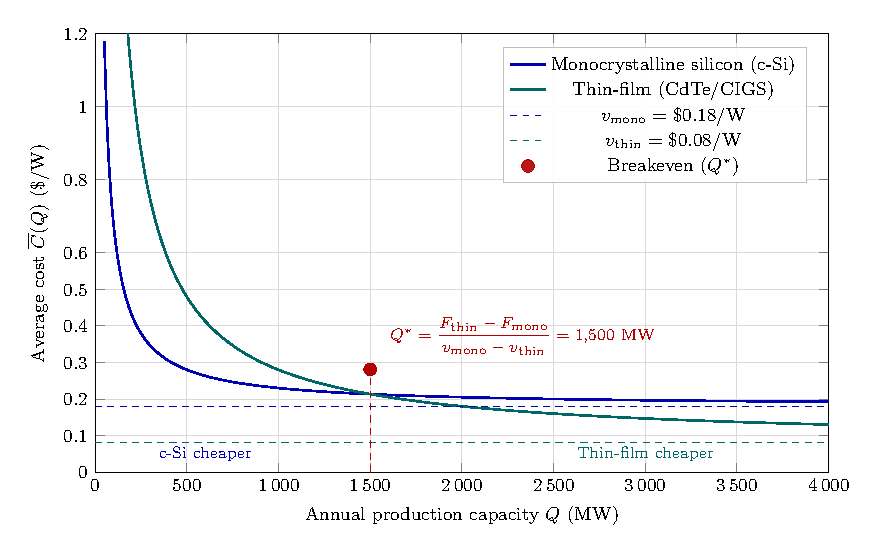
\includegraphics[width=0.5\linewidth]{Figures/lcoe_crossover.pdf}
    \caption{Thin-film is cheaper beyond a certain level of production.}
    \label{fig:Costs}
\end{figure}


\paragraph{Evidence of China's Supply-Side Policy Interventions}
China’s solar panel manufacturing grew rapidly over the sample period, with its global market share rising from under 2 percent in 2000 to more than 60 percent by 2011. This expansion was primarily driven by c-Si technology, which dominates Chinese production. See Figure \ref{fig:data_sum_China_output}(a) for China’s share of the global market and the output of the two solar panel technologies.

The price of polysilicon rose from 50 to 350 dollars per GW during the 2005-2008 surge. Globally, the market share of c-Si technology is sensitive to changes in polysilicon prices. In contrast, the predominance of c-Si in China did not react to this sharp input cost increase. This pattern indicates that China subsidized c-Si technology during this period.

Furthermore, the sharp increase in Chinese entrants aligns with government policy. Figure \ref{fig:data_sum_China_output}(b) shows the number of new entrants, exiting firms, and active solar panel producers in China over this period. Following the 2010 policy change that designated solar manufacturing as a strategic industry, market entry rose steeply; although firm exits also climbed, the overall number of firms still expanded substantially.

Taken together, these patterns suggest an important interaction between input price dynamics, policy interventions, and learning-by-doing, which jointly shape industry evolution. These features motivate the structural framework developed in the next section.

\begin{figure}[H]
\caption{Solar Panel Price and Installed Capacity}
\label{fig:data_sum_two_tech_price_output}
    \begin{center}
    \begin{subfigure}{.45\textwidth}
    \caption{Price}
    \centering
    
\includegraphics[trim=0.6in 3.4in 0.6in 2.5in, width=\textwidth]{Figures/Fig_data_sum_solar_panel_price.pdf}    
    \end{subfigure}   
    \hspace{0.5cm}
    \begin{subfigure}{.45\textwidth}
    \caption{Installed Capacity}
    \centering
    
\includegraphics[trim=0.6in 3.4in 0.6in 2.5in, width=\textwidth]{Figures/Fig_data_sum_solar_panel_installed_capacity.pdf}    
    \end{subfigure} 
    \end{center}
\vspace{0.5cm}
\footnotesize{ }
\end{figure}


\begin{figure}[H]
\caption{China's Market Share and Number of Firms}
\label{fig:data_sum_China_output}
    \begin{center}
    \begin{subfigure}{.45\textwidth}
    \caption{Market Share}
    \centering
    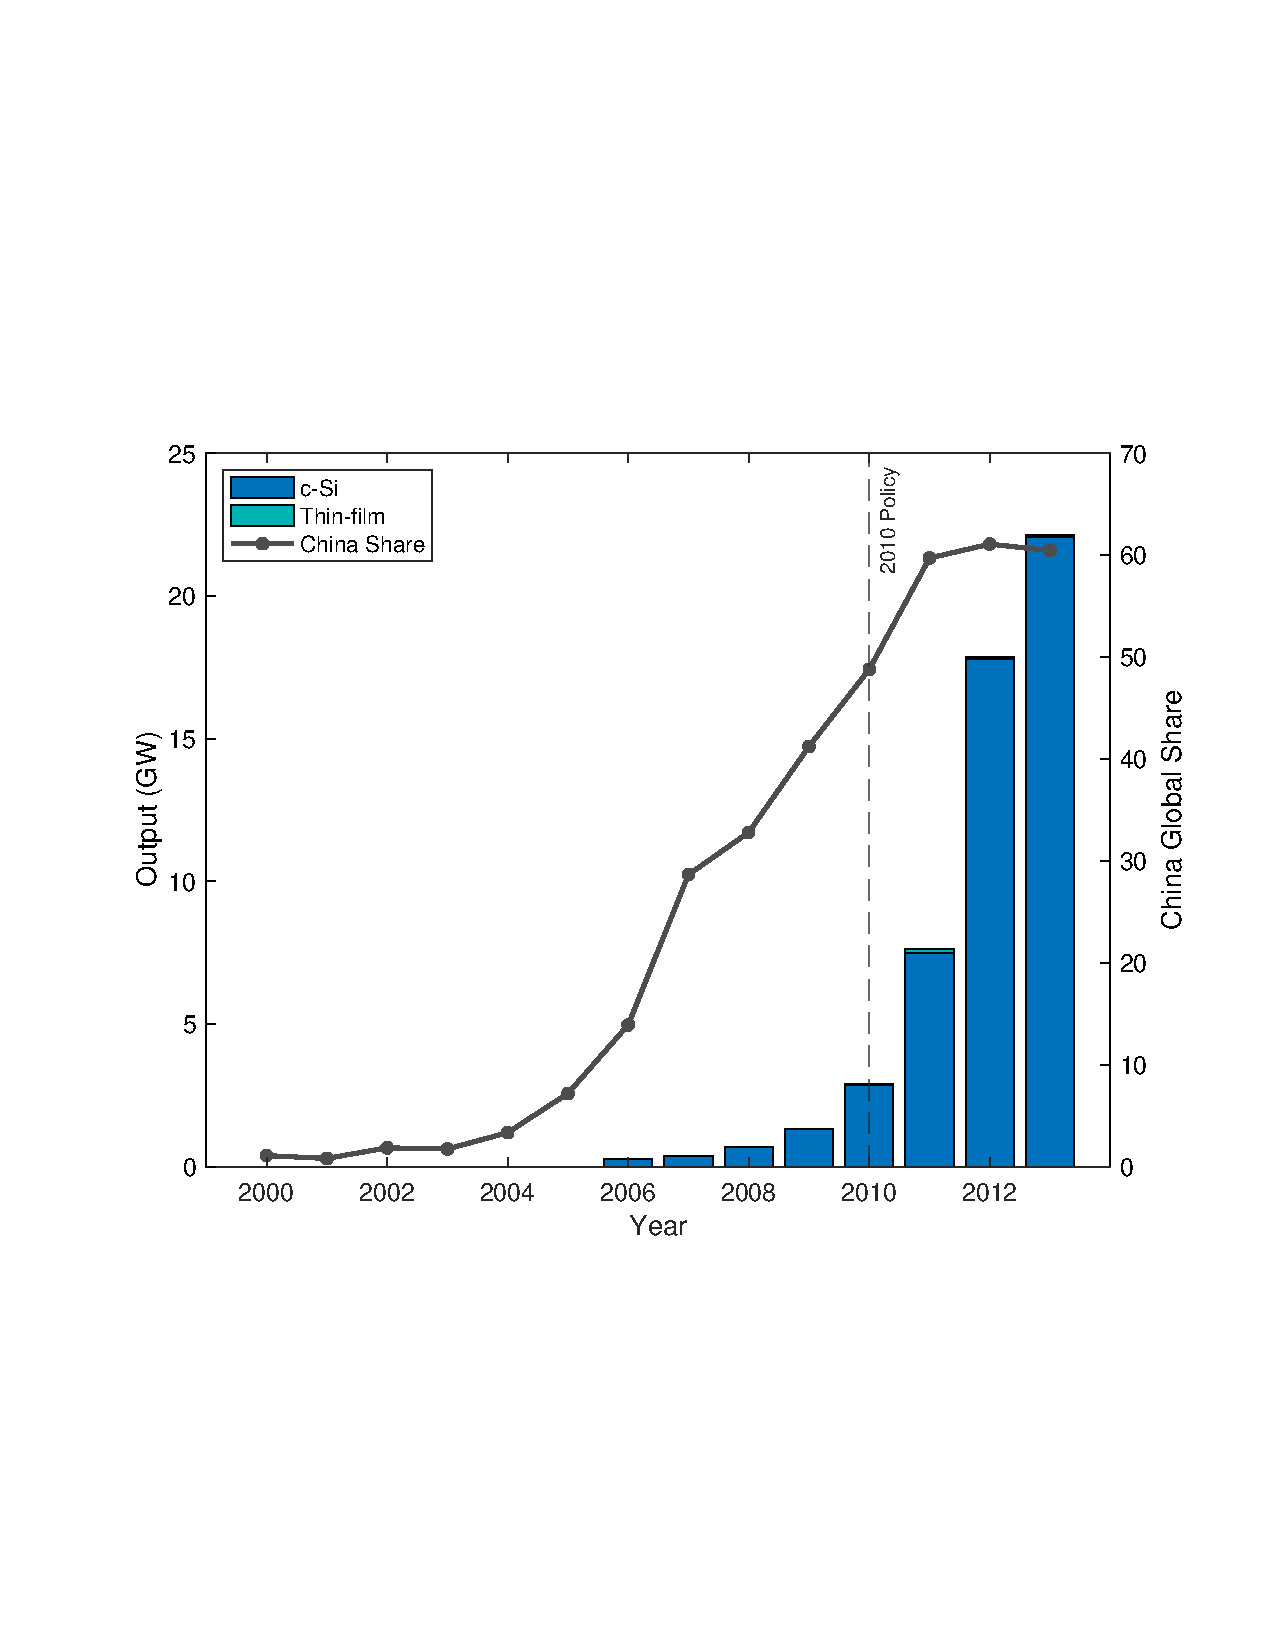
\includegraphics[trim=0.6in 3.4in 0.6in 2.5in, width=\textwidth]{Figures/Fig_data_sum_China_market_share.pdf}    
    \end{subfigure}   
    \hspace{0.5cm}
    \begin{subfigure}{.45\textwidth}
    \caption{Number of Firms}
    \centering
    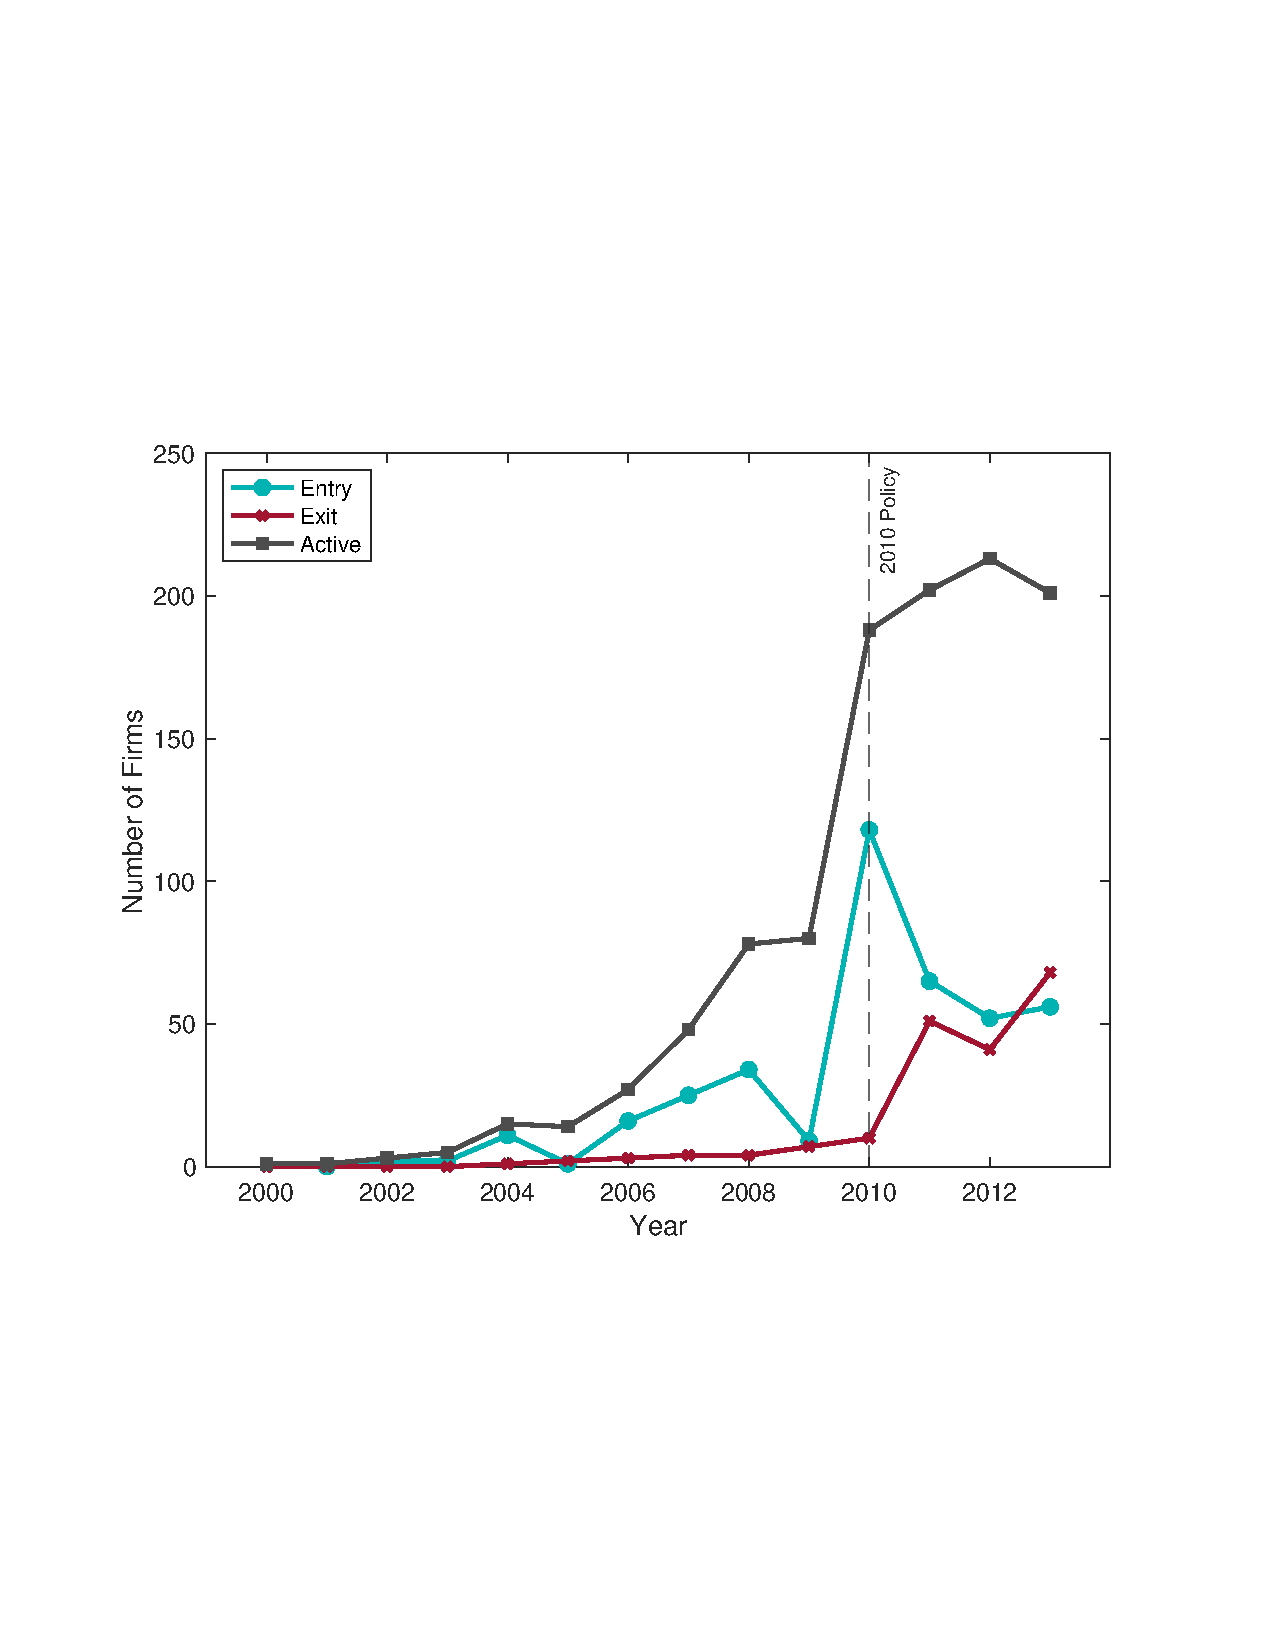
\includegraphics[trim=0.6in 3.4in 0.6in 2.5in, width=\textwidth]{Figures/Fig_data_sum_China_num_firms.pdf}    
    \end{subfigure} 
    \end{center}
\vspace{0.5cm}
\footnotesize{}
\end{figure}

\begin{figure}[H]
\caption{Polysilicon Price and Output}
\label{fig:data_sum_polysilicon}
    \begin{center}
    \begin{subfigure}{.45\textwidth}
    \caption{Price}
    \centering
    
\includegraphics[trim=0.6in 3.4in 0.6in 2.5in, width=\textwidth]{Figures/Fig_data_sum_polysilicon_price.pdf}    
    \end{subfigure}   
    \hspace{0.5cm}
    \begin{subfigure}{.45\textwidth}
    \caption{Output}
    \centering
    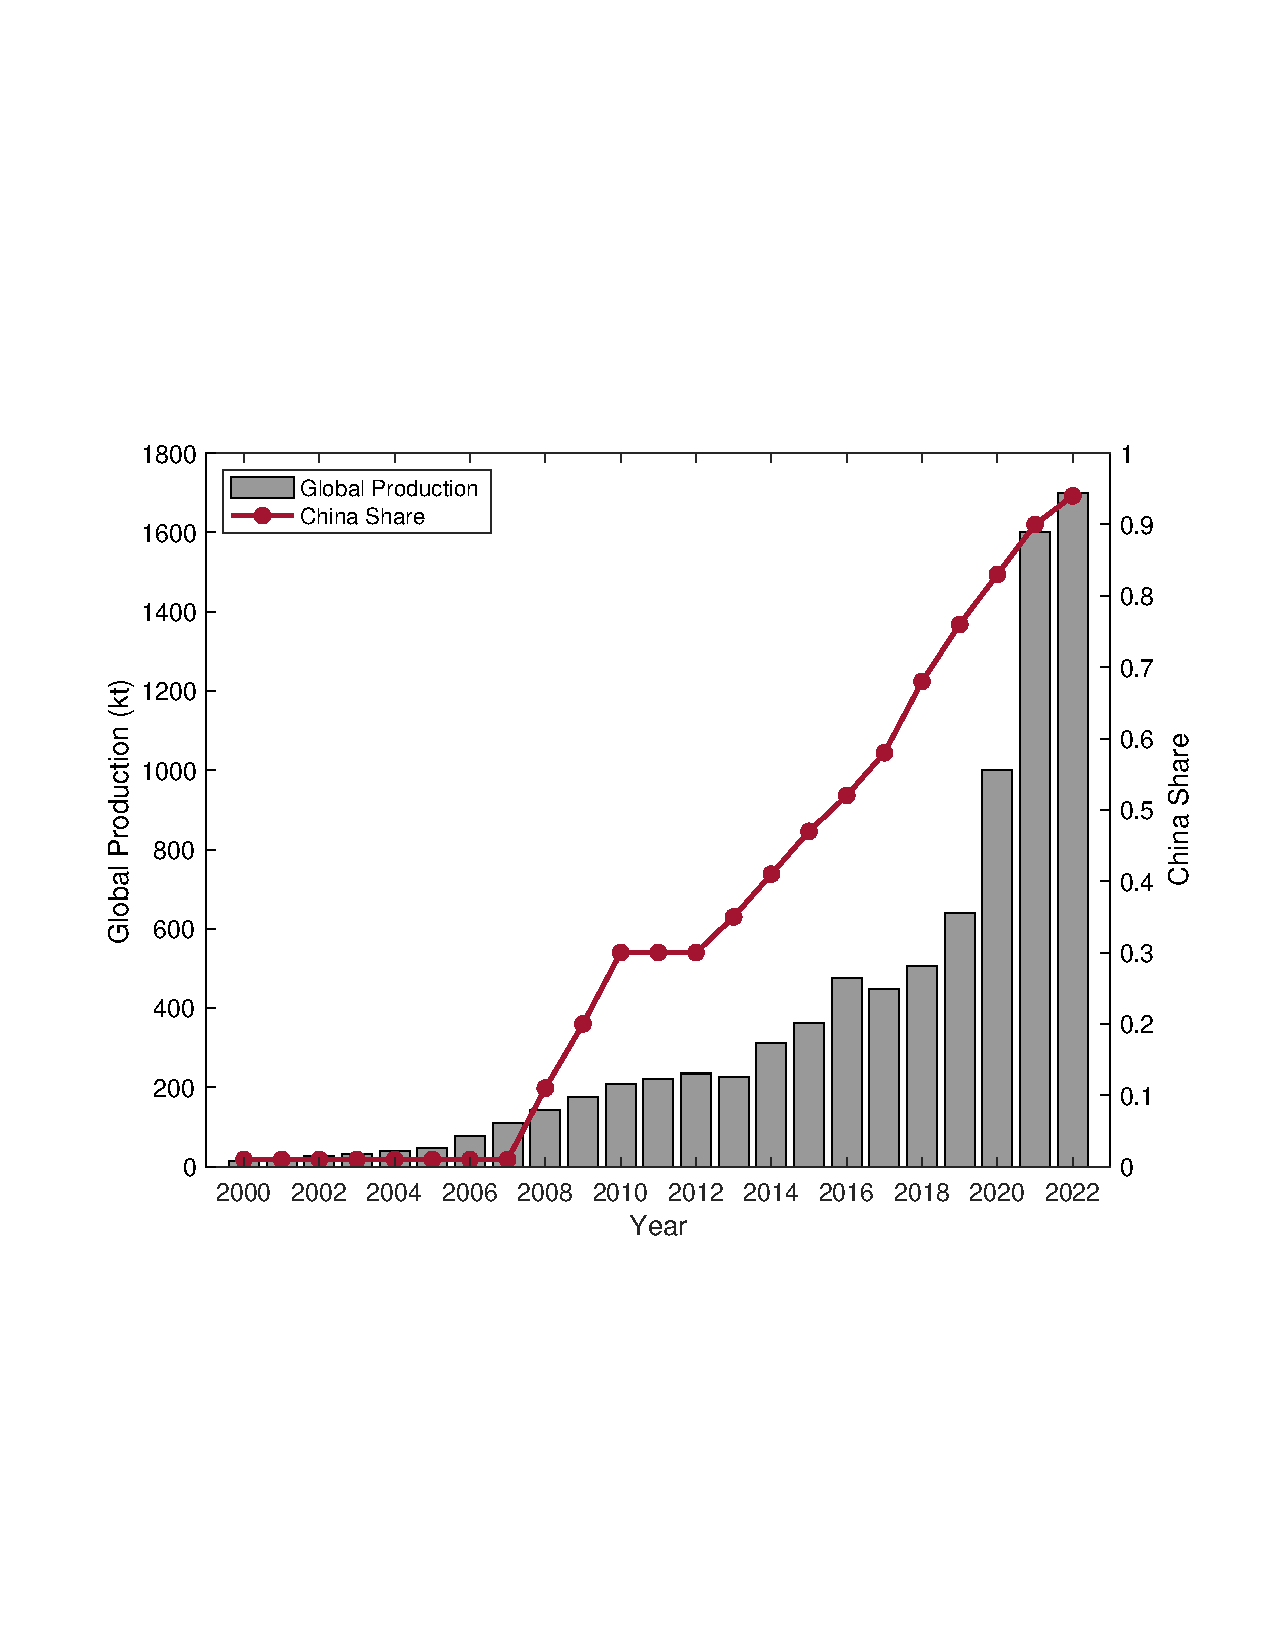
\includegraphics[trim=0.6in 3.4in 0.6in 2.5in, width=\textwidth]{Figures/Fig_data_sum_polysilicon_production.pdf}    
    \end{subfigure} 
    \end{center}
\vspace{0.5cm}
\footnotesize{}
\end{figure}

% Learning-by-doing amplifies the effects of industrial policies and input-price declines. Higher output increases cumulative production experience, which lowers future production costs and prices, generating a dynamic feedback loop.

% \begin{landscape}
% % Preamble (add if needed):
% \usepackage{tikz}
% \usetikzlibrary{arrows.meta,positioning,shapes.geometric}
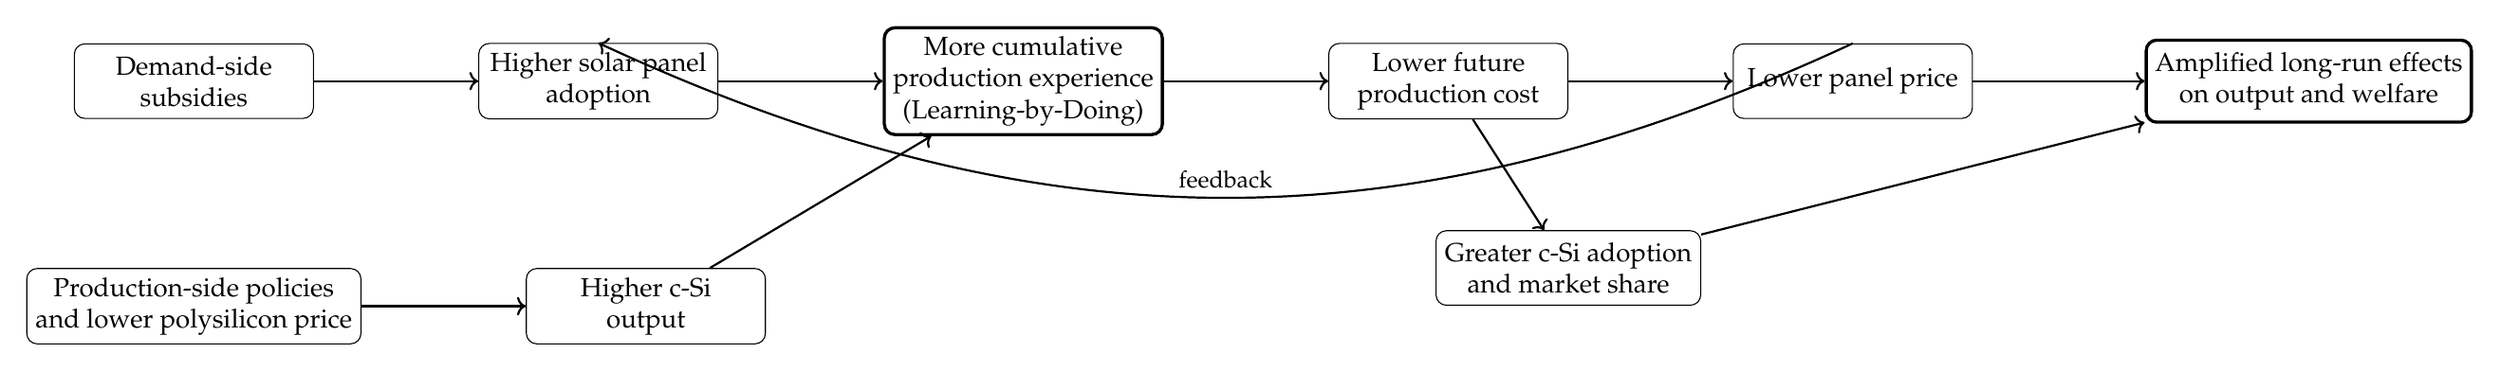
\begin{tikzpicture}[
    node distance=1.8cm and 2.2cm,
    box/.style={rectangle, draw, rounded corners, align=center, minimum width=3.2cm, minimum height=1cm},
    bigbox/.style={rectangle, draw, very thick, rounded corners, align=center, minimum width=3.6cm, minimum height=1.1cm},
    arrow/.style={->, thick}
]

% Top branch
\node[box] (demand) {Demand-side\\subsidies};
\node[box, right=of demand] (adopt1) {Higher solar panel\\adoption};
\node[bigbox, right=of adopt1] (lbd) {More cumulative\\production experience\\(Learning-by-Doing)};
\node[box, right=of lbd] (cost1) {Lower future\\production cost};
\node[box, right=of cost1] (price1) {Lower panel price};

% Bottom branch
\node[box, below=2cm of demand] (prod) {Production-side policies\\and lower polysilicon price};
\node[box, right=of prod] (output2) {Higher c-Si\\output};
\node[box, right=of cost1, below=2cm] (share) {Greater c-Si adoption\\and market share};

% Final outcome
\node[bigbox, right=2.3cm of price1] (welfare) {Amplified long-run effects\\on output and welfare};

% Arrows top
\draw[arrow] (demand) -- (adopt1);
\draw[arrow] (adopt1) -- (lbd);
\draw[arrow] (lbd) -- (cost1);
\draw[arrow] (cost1) -- (price1);
\draw[arrow] (price1) -- (welfare);

% Arrows bottom
\draw[arrow] (prod) -- (output2);
\draw[arrow] (output2) -- (lbd);
\draw[arrow] (cost1) -- (share);
\draw[arrow] (share) -- (welfare);

% Feedback loop
\draw[arrow, bend left=25] (price1.north) to node[above] {\small feedback} (adopt1.north);

\end{tikzpicture}
% \end{landscape}
% \begin{figure}
% \caption{LBD and Policies}
% \label{fig:lbd_mechanism}
% \centering
% % Preamble (add if needed):
% \usepackage{tikz}
% \usetikzlibrary{arrows.meta,positioning,shapes.geometric}
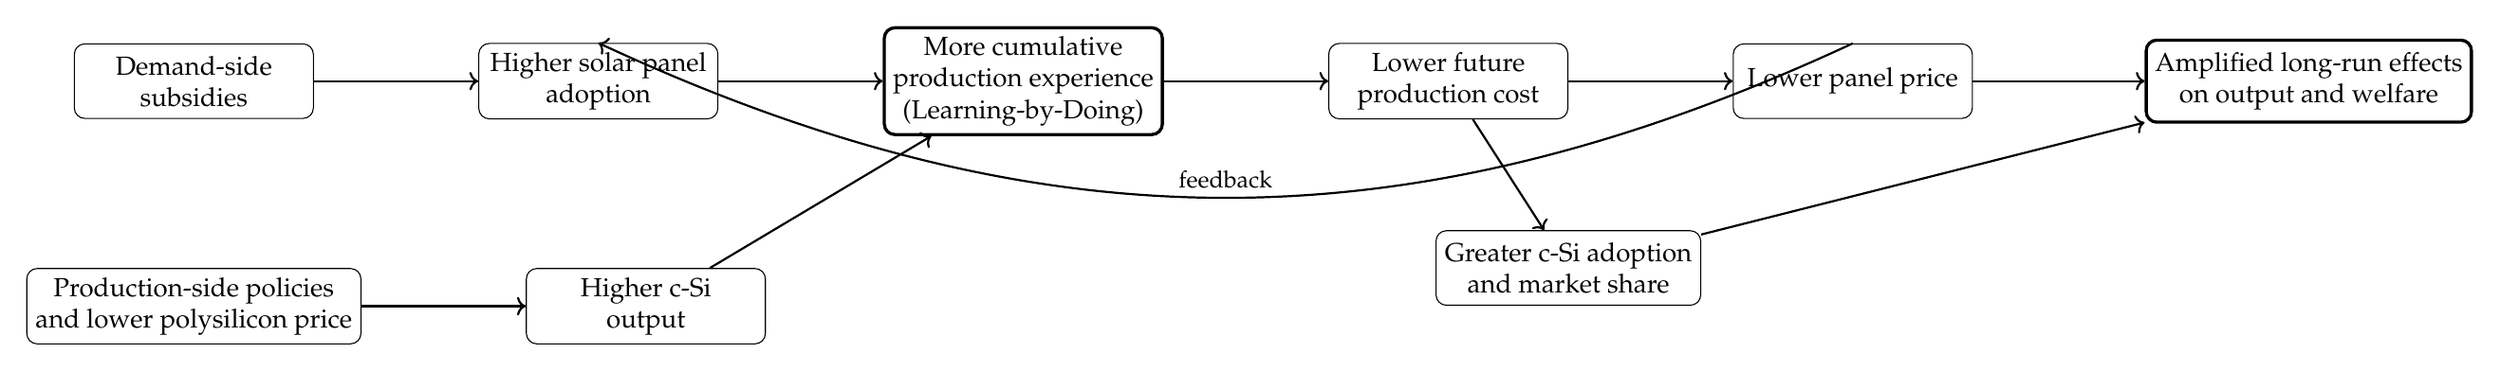
\begin{tikzpicture}[
    node distance=1.8cm and 2.2cm,
    box/.style={rectangle, draw, rounded corners, align=center, minimum width=3.2cm, minimum height=1cm},
    bigbox/.style={rectangle, draw, very thick, rounded corners, align=center, minimum width=3.6cm, minimum height=1.1cm},
    arrow/.style={->, thick}
]

% Top branch
\node[box] (demand) {Demand-side\\subsidies};
\node[box, right=of demand] (adopt1) {Higher solar panel\\adoption};
\node[bigbox, right=of adopt1] (lbd) {More cumulative\\production experience\\(Learning-by-Doing)};
\node[box, right=of lbd] (cost1) {Lower future\\production cost};
\node[box, right=of cost1] (price1) {Lower panel price};

% Bottom branch
\node[box, below=2cm of demand] (prod) {Production-side policies\\and lower polysilicon price};
\node[box, right=of prod] (output2) {Higher c-Si\\output};
\node[box, right=of cost1, below=2cm] (share) {Greater c-Si adoption\\and market share};

% Final outcome
\node[bigbox, right=2.3cm of price1] (welfare) {Amplified long-run effects\\on output and welfare};

% Arrows top
\draw[arrow] (demand) -- (adopt1);
\draw[arrow] (adopt1) -- (lbd);
\draw[arrow] (lbd) -- (cost1);
\draw[arrow] (cost1) -- (price1);
\draw[arrow] (price1) -- (welfare);

% Arrows bottom
\draw[arrow] (prod) -- (output2);
\draw[arrow] (output2) -- (lbd);
\draw[arrow] (cost1) -- (share);
\draw[arrow] (share) -- (welfare);

% Feedback loop
\draw[arrow, bend left=25] (price1.north) to node[above] {\small feedback} (adopt1.north);

\end{tikzpicture}
% \end{figure}


\begin{comment}
Table \ref{tab:data_sum} reports the summary statistics on key variables of interest of Chinese solar panel manufacturers.

\begin{table}[!h]
\centering
\caption{Summary Statistics on Chinese solar panel Manufacturers}
\label{tab:data_sum}
\begin{threeparttable}
\begin{tabularx}{0.7\textwidth}{Xcccccc}
\toprule
Variable & Mean & SD \\
\midrule
\multicolumn{3}{l}{\textit{c-Si solar panel:}} \\
%$\mathds{1}(\text{Polysilicon solar panel})$ &   &  \\
\quad Output (GW) &  65 & 300 \\
%\quad Investment (mill RMB) &  9.32 & 32.90 \\
\quad Capital (mill RMB) & 362  & 881 \\
\quad Age & 5.701  & 5.59 \\
\quad $\mathds{1}(\text{Private owned})$ & .435  & .496 \\
\quad $\mathds{1}(\text{Foreign JV})$ & .516 & .500 \\

\multicolumn{3}{l}{\textit{Thin-film solar panel:}} \\
%$\mathds{1}(\text{Polysilicon solar panel})$ &   &  \\
\quad Output (GW) & 24 & 70\\
%\quad Investment (mill RMB) & 9.59  & 17.1 \\
\quad Capital (mill RMB) & 455  &663  \\
\quad Age &  5.67 & 4.48 \\
\quad $\mathds{1}(\text{Private owned})$ & .112  & .317 \\
\quad $\mathds{1}(\text{Foreign JV})$ & .806  &  .397 \\
\bottomrule
\end{tabularx}
\begin{tablenotes}
  \item  Notes: This table includes 912 firm-year level observations of c-Si solar panel and 98 firm-year level observations of thin-film solar panel.
\end{tablenotes}
\end{threeparttable}
\end{table}
\end{comment}


\newpage


\section{Model}\label{sec:LBDmodel}
In this section, we present a dynamic model of firm entry, technology adoption, exit, and production. Time is discrete and a period is a year, denoted as $t$. There are two types of production technologies, indexed by $n\in\{1,2\}$, where $n=1$ denotes c-Si and $n=2$ denotes thin-film solar panels. The global market is divided into $m=1,...,m$ economic regions (China, EU, India, Japan, US, and rest of the world). At each period $t$, a set of firms produces solar panels. Firms are forward-looking and interact in a dynamic oligopoly environment with endogenous entry, exit, and production decisions.
%In any given period, there exist $j = 1,...,J_{nt}$ firms in the world that produce solar panels using technology $n$. 

At the beginning of each period, incumbent firms observe their scrap values and decide whether to exit the market. If they choose to stay, these incumbents observe their production cost shocks for each region and determine how many units to produce for each region. Meanwhile, potential entrants observe their entry shocks and decide on whether to enter and, if they do, choose which technology to adopt. 


% At the beginning of every year $t$, incumbent firms observe scrap value $\phi_{jnt}$ and decide whether to exit. Conditional on remaining active, incumbent firms observe production cost shocks for each region $\omega_{jnmt}$, choose how many units to produce for each region $q_{jnmt}$. Entrants observe entry shock $\zeta_{jnt}$, decide whether to enter and if entering, which technology to use.

\subsection{Per-Period Demand}
For each technology $n$ and region $m$, the aggregate demand is given by
\begin{equation}
Q_{nmt}=Q_{nm}(P_{1mt},P_{2mt},X_{mt}), \label{eq:model_demand}
\end{equation}
where $Q_{nmt}$ is the total quantity of technology-$n$ solar panels demanded by consumers in region $m$ during period $t$. The vector $X_{mt}$ includes a range of demand shifters, including measures of aggregate economic activity, regional fixed effects, and demand-side subsidies. The variable $P_{nmt}$ is the price consumers pay to install a technology $n$ solar panel system, incorporating both the retail panel price and installation expenses. This consumer price may differ from the global price $P_{nt}$ because of tariffs and installation subsidies that vary by region and technology. Specifically, the consumer price is given by:
\[P_{nmt} = P_{nt}\times (1 + \text{tariff}_{nmt}) + P^{I}_{mt} - \text{demand subsidy}_{mt},\]
where $\text{tariff}_{nmt}$ is the tariff rate, which applies only to c-Si technology, $P^{I}_{mt}$ is the installation expenses, and $\text{demand subsidy}_{mt}$ is the amount of demand-subsidies provided by region $m$ in period $t$.


\subsection{Incumbents: Production and Exit}
At the beginning of each period, incumbents observe their private scrap values that are drawn from a technology-specific distribution, and then decide to either exit or continue operations. We denote the scrap value for technology-$n$ incumbent $j$ as $\phi_{jnt}$ and its distribution as $F_{\phi,n}$. If a firm exits, it receives its scrap value. If it remains active, it observes its marginal cost shocks across all regions, denoted as $\boldsymbol{\omega}_{jnt} =\{\omega_{jnmt}\}_{m=1}^M$. Remaining active, firms engage in Cournot competition while considering how their current output decisions will influence future production costs. They simultaneously decide the quantity of solar panels to produce for each region, $\boldsymbol{q}_{jnt} = \{q_{jnmt}\}_{m=1}^M$, to maximize their discounted profit, taking as given the production decisions of rival firms. This new output, $\sum_{m=1}^M q_{jnmt}$, is added to the next period's accumulated experience, which in turn affects its future production costs.

\paragraph{Production Cost}
The production cost for firm $j$ using technology $n$, when choosing a vector $\boldsymbol{q}_{jnt}$, consists of two parts:
\begin{eqnarray}
   TC_{n}(\boldsymbol{q}_{jnt},s_{jnt},\boldsymbol{\omega}_{jnt})&=& C_0\!\left(\sum_{m=1}^M q_{jnmt},\; s_{jnt}\right) + \sum_{m=1}^M C_m\!\left(q_{jnmt},\; \omega_{jnmt}\right) \label{eq:model_c_q},
\end{eqnarray}
where the first component, $C_0\!\left(\sum_{m=1}^M q_{jnmt},\; s_{jnt}\right)$, represents the total production cost of $\sum_{m=1}^M q_{jnmt}$, which is a function of the current output and a vector of state variables $s_{jnt}$. These state variables include the firm's accumulated experience $e_{jnt}$, cost shifters that are common across firms (such as input prices), and technology-specific time trends that capture overall improvements in cost efficiency. %firm characteristics, and policy indicators that capture the effects of industrial policies on production costs. 
The second component, $C_m\!\left(q_{jnmt},\; \omega_{jnmt}\right)$, accounts for the additional cost of delivering $q_{jnmt}$ to destination $m$ in year $t$.

The experience of firm $j$, denoted as $e_{jnt}$, can potentially reduces production costs in the future, incentivizing the firm to increase output to gain more experience in the current period.  This experience is defined as the cumulative past production:
\[e_{jnt} = \sum_{\tau<t} \sum_m q_{jnm\tau},\]
where $q_{jnm\tau}$ is the units sold by firm $j$ to region $m$ during year $\tau$. The key parameter of interest is the experience coefficient, which measures how rapidly the unit cost of solar panel manufacturing falls as the production experience increases. 

\paragraph{Incumbent Value Function}
The value function of a technology-$n$ incumbent $j$, after observing the scrap value $\phi_{jnt}$ but before observing the realization of the production cost shock $\boldsymbol{\omega}_{jnt}$, is defined as:
\begin{eqnarray}
V_n(s_{jnt},\phi_{jnt})&=&\max\{\phi_{jnt},CV_n(s_{jnt})\},  \label{eq:incumbent_value_fn} 
\end{eqnarray}
where the continuation value $CV_n(s_{jnt})$  is expressed as:
\begin{eqnarray}
CV_n(s_{jnt}) & \equiv & \mathbb{E}_{\omega}\Big[ max_{\boldsymbol{q}} \{\sum_m P_{nm}(q_{m}, \boldsymbol{q}_{-mt},X_{mt}) q_{m} - TC_{n}(\boldsymbol{q},s_{jnt},\boldsymbol{\omega}_{jnt})  \nonumber \\
&& +\beta \mathbb{E}[V_n(s_{jnt+1})|s_{jnt}, \boldsymbol{q}] \}\Big]. \label{eq:incumbent_EV_fn}
\end{eqnarray}
Here, $\boldsymbol{q} = \{q_m\}_{m=1}^M$ is a vector of output choice for each region, while $\boldsymbol{q}_{-mt}$ denotes the output vectors that are chosen by other competing solar panel firms for region $m$. The expected value $\mathbb{E}_{\omega}$ is calculated with respect to the production cost shocks $\boldsymbol{\omega}_{jnt}$, 

\paragraph{Optimal Exit Decision}
The optimal decision to exit follows a threshold structure. A firm exits the market if the scrap value exceeds the continuation value; otherwise, it remains active. Therefore, the probability of exiting is:
\begin{eqnarray}
    p_n^x(s_{jnt}) & \equiv & Pr\!\left(\phi_{jnt} > CV_n(s_{jnt})\right) = 1-F_{\phi,n}\!\left(CV_n(s_{jnt})\right). \label{eq:exit_policy_fn}
\end{eqnarray}

\paragraph{Optimal Production Decision}
Provided that firm $j$ with technology-$n$ stays active, the optimal output level, $q_{jnmt}^*=q_{nm}^*(s_{jnt},\omega_{jnmt})$, satisfies the following first-order condition:
 \begin{eqnarray}
 \frac{\partial TC_{n}(\boldsymbol{q}_{jnt}^*,s_{jnt},\boldsymbol{\omega}_{jnt})}{\partial q_{jnmt}^*} & = & \underbrace{
    P_{nmt}+q_{jnmt}^*\frac{\partial P_{nm}(q^*_{jnmt}, \boldsymbol{q}^*_{-mt},X_{mt})}{\partial q_{jnmt}}}_{\text{Impact on current profit}} \nonumber \\
    && +  \underbrace{\beta \frac{\partial \mathbb{E}[V_n(s_{jnt+1})|s_{jnt}, \boldsymbol{q}_{jnt}^*] }{\partial q_{jnmt}} }_{\text{Impact on future profits via LBD}}, \label{eq:model_foc_q}
\end{eqnarray}  
where $\boldsymbol{q}^*_{-mt}$ denotes the vector of equilibrium outputs that are chosen by all other rival solar panel firms for region $m$ during year $t$. The firm’s optimal output is driven by three components: the first term captures its static profit margin, the second term captures its market power (the Cournot effect), and the third term captures the dynamic incentive arising from LBD. Because of this last component, firms may produce more than the static optimum in order to accumulate experience and lower their future costs.

\begin{comment}
\paragraph{Firm Profit}
Firm $j$'s expected profit before the production cost shocks are realized is given by:
\[
\pi_n(s_{jnt}) = \mathbb{E} [\sum_m \pi_{nm}(s_{jnt},\omega_{jnmt})]
\]
where $\pi_{nm}(s_{jnt},\omega_{jnmt})$ is firm $j$'s equilibrium profit from region $m$.
\end{comment}

\paragraph{Equilibrium Global Price}
In each period, the global price of technology-$n$ solar panels, denoted as $P_{nt}$, equates the aggregate demand and supply, where the aggregate demand is described by equation \eqref{eq:model_demand} and the aggregate supply is the sum of $q_{jnmt}^*$ defined in equation \eqref{eq:model_foc_q} across all firms using technology $n$.  
%\textcolor{blue}{We only have data on the Chinese firms, rather than all firms in the world. It is biased to use a subset of firms to compute the global price that equalizes the total supply and total demand.}

\subsection{Potential Entrants: Entry and Technology Selection}
At the end of each period $t$, a total of $\bar N$ potential entrants observe their payoff $\zeta_{j0t}$ for not entering, as well as entry costs $\kappa_1(s_{jnt})-\zeta_{j1t}$ for entering with c-Si technology, and $\kappa_2(s_{jnt})-\zeta_{j2t}$ for entering with thin film technology. The terms $\kappa_1(s_{jnt})$ and $\kappa_2(s_{jnt})$ denote the expected entry costs associated with the two technologies. The vector $s_{jnt}$ includes policy dummies to capture the impact of industrial policies on the decisions regarding entry and technology selection.

After observing their entry payoff shocks $\zeta$'s, potential entrants decide whether to enter the market and, if they choose to enter, select a technology. If they opt to enter, they incur the entry cost during the current period and start earning profit from the product market starting from the following period. Therefore, the maximization problem of the potential entrant $j$ can be written as:
\begin{eqnarray}
 && max\Big\{\zeta_{j0t}, \; max_{n\in \{1,2\}} \{-\kappa_n(s_{jnt}) + \zeta_{jnt} + \beta \mathbb{E}[V_n(s_{jnt+1}) \mid s_{jnt}]\} \Big\}
\end{eqnarray}

A firm stays out of the market if its payoff from not entering exceeds the expected profit of entering with either technology option. It chooses to enter with technology $n$ if this option provides the highest profit. We use $p^{e,n}(s_{jnt})$ to denote the probability that a potential entrant $j$ enters with technology $n$, given by
\begin{eqnarray}
  p^{e,n}(s_{jnt}) & \equiv & \text{Pr}\Big\{\zeta_{jnt} - \zeta_{jn't}  > \kappa_n(s_{jnt})-\kappa_{n'}(s_{jn't}) + \beta \mathbb{E}[V_{n'}(s_{jn't+1}) \mid s_{jn't}] - \beta \mathbb{E}[V_n(s_{jnt+1}) \mid s_{jnt}] \nonumber \\
  & & \quad  \& \  \zeta_{jnt}-\zeta_{j0t} + >\kappa_n(s_{jnt})-\beta \mathbb{E}[V_n(s_{jnt+1}) \mid s_{jnt}] \Big\} \label{eq:entry_policy_fn}
\end{eqnarray}
Note that LBD affects entry decisions through the expected value term $\mathbb{E}[V_n(s_{jnt+1}) \mid s_{jnt}]\}$. A technology with stronger learning becomes more attractive dynamically, even if it is initially costly.


\subsection{Markov-Perfect Equilibrium}
A Markov-Perfect Equilibrium is characterized by policy function, $q^*_{nm}(s_{jnt}$, $\omega_{jnmt})$, $p_n^x(s_{jnt})$, $p_n^e(s_{jnt})$, value function $V_n(s_{jnt})$, and global price $P_{nt}$, such that production policy function $q^*_{nm}(s_{jnt},\omega_{jnt})$ satisfies \eqref{eq:model_foc_q}, exit policy function $p_n^x(s_{jnt})$ satisfies \eqref{eq:exit_policy_fn}, entry policy function $p_n^e(s_{jnt})$ satisfies \eqref{eq:entry_policy_fn}, global price $P_{nt}$ ensures that aggregate demand and aggregate supply are in balance, while the incumbent's value function $V_n(s_{jnt})$ satisfies \eqref{eq:incumbent_value_fn}.

\subsection{Model Discussion}
The model highlights a central mechanism of the paper: policies affect output not only directly, but also indirectly by changing the accumulation of production experience. This generates a dynamic feedback loop in which higher output reduces future costs, amplifying the long-run effects of policies. %Importantly, our framework allows LBD to amplify the effects of both input price shocks and policy interventions. This amplification arises because higher output today increases future productivity, generating dynamic complementarities that are central to our counterfactual analysis.

Before moving on to the estimation, we discuss two key simplifying assumptions made by our model. 
%First, we assume that solar panels are homogeneous conditional on their production technology. This assumption is consistent with the highly commoditized nature of solar panels. In addition, \cite{bollinger2025strategic} analyze a dataset of solar panel shipments to the United States, constructed from quarterly IHS Markit data, and document very little price dispersion across manufacturers at any given time.
First, production cost shocks $\omega_{jnmt}$ are assumed to be i.i.d., because allowing for a persistent time-varying unobserved state variable in a dynamic model would introduce substantial computational complexity. Nonetheless, our model does incorporate persistent effects through the accumulation of experience. When firms receive positive demand shocks, they increase quantity, which in turn increases their stock of experience.  Since experience is a state variable, firms with more experience have lower production costs and thus choose higher output levels, further building experience and reducing long-run costs. This feedback mechanism is the key driver of why firms that are ex-ante identical can exhibit divergent growth paths over time.

Second, following most of the existing literature such as \citet{ryan2012costs} and \citet{barwick2025industrial}, we assume that all firms view government policies as permanent.  Relaxing this assumption would require modeling firms’ expectations and their adjustment to a changing policy environment, which would greatly increase the complexity of our analysis. This is an important avenue for future research; see \citet{gowrisankaran2025policy} and \citet{chen2024dynamic} for further discussion.


\section{Estimation Strategy}\label{sec:LBDestimation}
In this section, we outline the strategy for estimating model parameters. In Section \ref{subsec:est_specifications}, we detail our demand model, specify the production cost function, as well as the distributions related to the scrap value and entry costs. In sections \ref{subsec:est_dynamic_first} and \ref{subsec:est_dynamic_second}, we present the two-stage procedure for estimating dynamic parameters, including those associated with the production cost function and the distributions for the scrap value and entry cost shocks.

We estimate the dynamic parameters using the firms' observed choices of production, exit, and entry, including not entering, entering with c-Si technology, or entering with thin-film technology. Using the BBL approach from \citet{bajari2007estimating}, we estimate these parameters in two stages. In the first stage, we flexibly estimate policy functions, including production, exit, and entry with technology selection, as well as the transition process of state variables directly from the data. After that, we approximate the value function using a set of B-spline basis functions of state variables, as described in (\citet{sweeting2013dynamic}). In the second stage, we estimate the dynamic parameters. We provide additional details in Appendix \ref{appendix:second_stage}.

\subsection{Specifications}
\label{subsec:est_specifications}

\paragraph{Logit Demand.}
We parameterize the solar panel demand, expressed in \eqref{eq:model_demand}, using a simple Logit model. To be specific, the demand of technology-$n$ solar panels in the region $m$ during the year $t$ is given by:
\begin{eqnarray*}
Q_{nmt} & = & \frac{M_{mt}\cdot exp(-\alpha_{m} P_{nmt} + X_{mt}\eta +\xi_{nmt})}{1+\sum_{n'}exp(-\alpha_{m} P_{n'mt} + X_{mt}\eta +\xi_{n'mt})}.  \label{eq:demand_specification}
\end{eqnarray*}
Here, $M_{mt}$ is the market size for region $m$ in year $t$, measured by the total electricity consumption. $P_{nmt}$ is the price of technology-$n$ solar panels that is faced by consumers in region $m$, calculated by adjusting the global price $P_{nt}$ with local installation cost, tariffs, and subsidies. $X_{mt}$ is a vector of demand shifters, including GPD, feed-in tariff, regional fixed effects, and yearly fixed effects. 

For the given demand, the estimation equation is represented as:
\begin{eqnarray}
ln( \frac{Q_{nmt}}{M_{mt}} ) - ln( \frac{M_{mt}- Q_{1mt}- Q_{2mt}}{M_{mt}} ) & = &  -\alpha_{m} P_{nmt} + X_{mt}\eta +\xi_{nmt}. \label{eq:demand_est_mkt}
\end{eqnarray}
A key challenge is price endogeneity, since prices respond to demand shocks $\xi_{nmt}$. To address this issue, we follow \citet{bollinger2025strategic} and instrument solar panel prices using global prices of silver and aluminum, which are key inputs in both c-Si and thin-film solar technologies but plausibly exogenous to regional demand shocks. Our identification relies on the assumption that variation in these input prices shifts production costs without directly affecting local demand conditions. This assumption is plausible because solar manufacturing in total represents less than 5\% of global demand for these inputs throughout the sample period.



\paragraph{Production Costs} 

% As shown in \eqref{eq:model_c_q}, the production cost function for firm $j$ of technology-$n$ is decomposed into two components, specified as
% \begin{eqnarray*}
%    C_0\!\left(\sum_m q_{jnmt},s_{jnt}\right) &=& (\gamma_{n}^0 + s_{jnt} \gamma_n^s) \cdot (\sum_m q_{jnmt}) + \frac{\gamma^{scale}}{2} \cdot (\sum_m q_{jnmt})^2,
% \end{eqnarray*}
% and
% \begin{eqnarray*}
%    C_m(q_{jnmt},\omega_{jnmt}) &=& (\gamma_{m}^{ex}+\omega_{jnmt}) \cdot q_{jnmt}.
% \end{eqnarray*}
% Here, $\gamma_{n}^0$ are technology-specific constants, while the parameters $\gamma_n^s$ capture how state variables affect the unit cost for a specific technology. The parameter $\gamma^{scale}$ captures the curvature of the cost function. The parameters $\gamma_{m}^{ex}$ are region-specific and represent the additional cost associated with shipping or exporting to that region. Finally, $\omega_{jnmt}$ are cost shocks, which are assumed to follow an independent and identically distributed normal distribution with a mean of zero and a variance of $\sigma_\omega^2$.

% As a result, the marginal cost that firm $j$ ships $q_{jnmt}$ to region $m$ is
% \begin{eqnarray*}
%   \frac{\partial TC_{jnt}}{\partial q_{jnmt}} &=&  \gamma_{n}^0 + s_{jnt} \gamma_n^s + \gamma^{scale} q_{jnmt}  +\gamma_{m}^{ex}  +\omega_{jnmt}. 
% \end{eqnarray*}

As specified in \eqref{eq:model_c_q}, the production cost function for firm $j$ using technology $n$ is decomposed into two components. The first component, $C_0\!\left(\sum_m q_{jnmt},s_{jnt}\right)$, is a function of the firm’s aggregate current output $\sum_m q_{jnmt}$ and the state variables $s_{jnt}$. The second component, $C_m(q_{jnmt},\omega_{jnmt})$, represents the additional cost of supplying quantity $q_{jnmt}$ to destination $m$ in year $t$.
Specifically, we specify the marginal cost function as
\begin{eqnarray}
  MC(q_{jnmt}) &=& \gamma^{e}_{jn} \cdot ln(e_{jnt}+1) + \; \mathbf{1}(n = \text{c-Si}) \cdot \text{polysilicon cost}_t  \nonumber \\
  & & + \;  \gamma_{n}^{\text{const}} + \gamma^{scale} q_{jnmt} +  \gamma^{time}_n \cdot\ln(t-1999)+\gamma_{m}^{ex}  + \omega_{jnmt} \label{eq:est_mc_q}
\end{eqnarray}
In this specification, the LBD term is modeled as the logarithm of one plus the firm’s cumulative experience, $ \ln(e_{jnt}+1) $, and the learning rate is denoted by $\gamma^{e}_{jn}$. This learning rate is specific to each technology. For c-Si firms, we additionally allow the learning rate to vary across firms; in particular, larger firms may learn more quickly.  More formally, the learning parameter is given by
\begin{eqnarray*}
\gamma^{e}_{jn} & = & \mathbf{1}(n = \text{thin-film}) \cdot \gamma^{e,\;\text{baseline}}_{\text{thin-film}} \nonumber \\
& & + \; \mathbf{1}(n = \text{c-Si}) \cdot (\gamma^{e,\;\text{baseline}}_{\text{c-Si}} + \mathbf{1}(j \in \text{large c-Si firms})\cdot \gamma^{e,\;\text{large}}_{\text{c-Si}}).
\end{eqnarray*}

For c-Si technology, the key input price is that of polysilicon, its primary input.  To account for the declining input-to-output conversion rate over this period, we introduce a time trend.\footnote{\cite{BernreuterResearch2020} documents that the polysilicon intensity (grams per watt) declined from above 20 g/W in the early 2000s to below 6 g/W by the early 2010s. The decline in conversion rate during this period was driven by a combination of process innovation, material efficiency, and performance improvements along the silicon solar value chain. First, wafer thickness fell substantially, reducing the amount of silicon required per cell. Second, manufacturing technologies improved, especially the transition toward more efficient wire-sawing methods, which sharply reduced kerf loss (silicon wasted during slicing). Third, cell and module efficiencies increased, meaning more electrical output (watts) could be generated from the same physical amount of silicon. Fourth, scale expansion and standardization (e.g., larger wafers and better yield management) further improved material utilization.}  In addition, as discussed in Section~\ref{sec:institution_data}, Chinese firms likely benefited from subsidies during the 2006–2008 surge in polysilicon prices. We therefore include subsidy parameters to represent input cost subsidies in those years.
Specifically, the input cost is
\begin{eqnarray}
\text{polysilicon cost}_t & = & \gamma^{i,\;\text{baseline}}_{\text{c-Si}} \cdot exp(\gamma^{i,\;\text{time}}_{\text{c-Si}} \cdot (t-2000)) \cdot \text{polysilicon price}_{t} \nonumber \\
&&-\sum_{t=2005}^{2008} \gamma^{i,\text{sub}}_{\text{c-Si},\;t} \cdot \mathbf{1}(t \in [2005,\;2008]),
\end{eqnarray}
where the parameter $\gamma^{i,\;\text{const}}_{\text{c-Si}}$ represents this conversion rate in the year 2000, $\gamma^{i,\;\text{time}}_{\text{c-Si}}$ captures the time trend reflecting aggregate efficiency improvements over this period, and $\gamma^{i,\text{sub}}_{\text{c-Si},\;t}$ denotes the per-watt subsidy provided to offset the input cost surge during the period of elevated polysilicon prices.

The parameter $\gamma_{n}^{\text{const}}$ represents the baseline cost level in the year 2000 for each of the two technologies. The term $\gamma^{scale}$ characterizes the curvature of the marginal cost function with respect to current output. The technology-specific time trend parameter $\gamma^{time}_n$ captures additional gains in cost efficiency over the sample period, excluding learning-by-doing effects and the polysilicon-to-module conversion. The parameters $\gamma_{m}^{ex}$ are region-specific and capture the extra costs related to shipping or exporting to each region. Finally, $\omega_{jnmt}$ are cost shocks, assumed to be independently and identically normally distributed with mean zero and variance $\sigma_\omega^2$.

\paragraph{Distributions of Scrap Value and Entry Costs.} 
We assume that the scrap value $\phi_{jnt}$ follows an exponential distribution characterized by a parameter $1/\sigma_{\phi}$. %\textcolor{blue}{(Note: we can allow the parameter to differ across the two technologies, $1/\sigma_{\phi,n}$)}.
Additionally, we assume that the entry cost shocks $\zeta$ are independently and identically distributed according to a Type 1 Extreme Value (T1EV) distribution.

\subsection{First Stage: Policy Functions and State Transition}
\label{subsec:est_dynamic_first}
Following the BBL approach, we first estimate firms’ decision rules directly from the data without imposing parametric structure on dynamic optimization.

\paragraph{Exit Policy Function} 
We estimate the exit policy function using a Probit specification:
\begin{eqnarray}
     Pr_n(\chi_{jnt} &=&1|s_{jnt})=\Phi(h_n(s_{jnt})), \label{eq:est_exit}
\end{eqnarray}
where the variable $\chi_{jnt}=1$ indicates the exit of firm $j$ with technology $n$ from the market in period $t$. Here, $h_n(s_{jnt})$ is a polynomial function of the states tailored to the specific technology, and $\Phi$ is the cumulative distribution function of a standard normal distribution. We use $\hat{p}^x_n(s)$ to refer to the estimated exit probability given state $s$.


\paragraph{Production Policy Function}
Similar to the optimal investment in \citet{bajari2007estimating}, the production policy function $q_{nm}^*(s_{jnt},\omega_{jnmt})$ decreases monotonically with the cost shock $\omega_{jnmt}$ and can be recovered as follows:
\begin{eqnarray}
q_{nm}^*|s_{jnt} &=& G_{nm}^{-1}(1-F_{\omega}(\omega\mid s_{jnt})), \label{eq:est_output_1}
\end{eqnarray}
where $G_{nm}(q\mid s_{jnt})$ is the empirical distribution of production given the state variables, and $F_{\omega}(\omega\mid s_{jnt})$ is the assumed distribution of $\omega$.

We can write the optimal production as the sum of two components: one depends only on the state variables, and the other depends only on the shock. Formally, this can be expressed as:
\begin{eqnarray}
q_{jnmt}^* &=& h_{1nm}(s_{jnt})+h_{2nm}(\omega_{jnmt}),\label{eq:est_output_2}
\end{eqnarray}
where $h_{1nm}(\cdot)$ and $h_{2nm}(\cdot)$ are two unknown functions that need to be estimated.

We first perform a flexible non-parametric regression of $q_{jnmt}$ on $s_{jnt}$ to get the estimate $\hat{h}_{1nm}(s_{jt})$, which allows us to compute $q^*_{jnmt}-\hat{h}_{1nm}(s_{jnt})$. Then, we estimate $h_{2nm}(\cdot)$ using equation (\ref{eq:est_output_1}).

\paragraph{State Transition}
The vector of state variables $s_{jnt}$ includes the state of all firms in the industry, making it high-dimensional. %Some of the state variables, such as firm location and ownership status, are fixed over time. The firm age transits deterministically. 
For experience stock, it transits as follows:
\[
e_{jnt+1}  =  e_{jnt} + \sum_m q_{jnmt}.
\]
where $\sum_m q_{jnmt}$ is the total production of firm $j$ during year $t$.

To reduce dimensionality, we assume that firms do not keep track of each competitor's state variables, but instead rely on industry-level prices as a sufficient statistic, akin to the oblivious equilibrium concept introduced by (\citet{weintraub2008markov} and \citet{benkard2015oblivious}). This assumption is justified given that the industrial HHI in China in 2013 being 316, indicating that market power is not a significant issue. This approach has often been adopted in the literature, for example, \citet{jeon2022learning}, \citet{chen2023structural}, and \citet{barwick2025industrial}.

However, the equilibrium price for each type of solar panel clears the market by equalizing aggregate demand and aggregate supply of that type of solar panel, which makes it a complicated object. Following \citet{barwick2025industrial} and other studies, we model them as AR(1) processes. We account for different technologies having different price processes. Furthermore, we incorporate changes in constant terms across different periods. We make similar assumptions for input prices. 
%\textcolor{blue}{
%We estimate the following AR(1) processes:
%\[
%y_t = \lambda_0^{pre} + \lambda_0^{post} \mathds{1}(t is post) + \lambda_1 y_{t-1} + \lambda_2 (t-t_0) + e_t,
%\]
%where $t_0$ indexes the first year of the sample, $y_t$ refers to the state variable in year $t$ including the price of c-Si %solar panels, price of thin-film solar panels, price of inputs, and demand subsidies.
%}

\subsection{Second Stage: Structural Estimation}
\label{subsec:est_dynamic_second}
In the second stage, we recover structural parameters by exploiting the optimality conditions implied by firms’ dynamic problem.

\subsubsection{Value Function Approximation}
The ex-ante value function, prior to the realization of $\phi_{jnt}$, is described by
\begin{eqnarray}
    V_n(s_{jnt}) & = & \mathbb{E}_\phi[ max\{\phi_{jnt},CV_n(s_{jnt})\}] = p_n^x(s_{jnt}) \sigma_\phi + CV_n(s_{jnt}), \label{eq:est_bellman}
\end{eqnarray}
where $p_n^x(s_{jnt})$ denotes the exit probability, and $CV_n(s_{jnt})$ denotes the continuation value as defined in equation (\ref{eq:incumbent_EV_fn}).

Following the existing literature (e.g., \citet{sweeting2013dynamic}), we approximate the ex-ante value function using B-spline basis functions of the state variables. This is expressed as $V_n(s_{jnt}) = \sum_l \rho_{n,l} u_{n,l}(s_{jnt})$ where $u_{n,l}(s_{jnt})$ are basis functions and $\rho_{n,l}$ are coefficients that need to be estimated along with the dynamic parameters.

Specifically, we search for coefficients $\rho$ that minimize the violation of the Bellman equation (\ref{eq:est_bellman}) given the dynamic parameters, given by
\begin{eqnarray}
     &  & min_{\rho} \Vert V_n(s_{jnt};\rho) -\hat{p}^x_n(s_{jnt}) \sigma_{\phi} - CV_n(s_{jnt};\rho)\Vert_2.\label{eq:est_value_func_approx}
\end{eqnarray}
Here, $\Vert \cdot \Vert_2$ is the $L^2$ norm, $\hat{p}^x_n(s_{jnt})$ is the estimated first-stage exit policy function, and the continuation value is evaluated based on these estimated policy functions, given by
\begin{eqnarray*}
CV_n(s_{jnt};\rho) & = & \mathbb{E}_{\omega} \Big[ \sum_m P_{nmt} \hat{q}^*_{nm}(s_{jnt},\omega_{jnmt}) - TC_{jnt}(\hat{q}^*_{nm}(s_{jnt},\omega_{jnmt}),s_{jnt},\omega_{jnt}) \\
&& + \beta \mathbb{E}[V(s_{jnt+1};\rho)\mid s_{jnt}, \hat{q}^*_{jnmt}] \Big],
\end{eqnarray*}
where $\hat{q}^*_{nm}(s_{jnt},\omega_{jnmt})$ is the estimated first-stage production policy function.

\subsubsection{Estimation of Production Costs and Scrap Value}

\paragraph{Log-Likelihood of Output}
The optimal output $q^*_{jnm}(s_{jnt},\omega_{jnmt})$ is determined by the first-order conditions in equation (\ref{eq:model_foc_q}). By construction, $q^*_{jnm}(s_{jnt},\omega_{jnmt})$ is strictly monotonic in $\omega_{jnmt}$. Assuming it is also differentiable,  the likelihood of output can be expressed as
\begin{eqnarray}
    g_{nm}(q_{jnmt};\theta) &=& \frac{f_\omega(\omega_{jnmt})}{|\partial q_{nm}^*(s_{jnt},\omega_{jnmt}) /\partial \omega_{jnmt}|},\label{eq:est_log_likelihood_output}
\end{eqnarray}
where $|\partial q_{nm}^*(s_{jnt},\omega_{jnmt}) /\partial \omega_{jnmt}|$ is the absolute value of the derivative of $q_{nm}^*(s_{jnt},\omega_{jnmt})$ with respect to $\omega_{jnmt}$.

\paragraph{Log-Likelihood of Exiting}
Let $\chi_{jnt}$ indicate that firm $j$ of technology $n$ exits in year $t$ in the data. The maximum likelihood estimate of the standard deviation scrap value, $\sigma_\phi$, maximizes the following log-likelihood for exit decisions:
\begin{eqnarray}
    log(f_n(s_{jnt};\theta)) &=& \Big[ (1-\chi_{jnt}) log(1-exp(-\frac{CV_n(s_{jnt};\rho)}{\sigma_\phi})) - \chi_{jnt} \frac{CV_n(s_{jnt};\rho)}{\sigma_\phi} \Big]. \label{eq:est_log_likelihood_exit}   
\end{eqnarray}

%\paragraph{GMM}

\subsubsection{Estimation of Entry Costs}
The probability that potential entrant $j$ enters with technology $n$ is expressed as
\begin{eqnarray}
  p^{e,n}(s_{jnt}) & \equiv & \frac{exp\Big(-\kappa_n(s_{jnt}) + \beta \mathbb{E}[V_n(s_{jnt+1}) \mid s_{jnt}] \Big)}{1 + \sum_{n'} exp\Big(-\kappa_{n'}(s_{jn't}) + \beta \mathbb{E}[V_{n'}(s_{jn't+1}) \mid s_{jn't}]\Big)}. %\label{eq:entry_policy_fn}
\end{eqnarray}
We estimate the mean entry costs using the observed entry decisions via MLE.

\subsection{Identification}
The central parameter of interest is the effect of experience on production cost. The identification of LBD relies on three distinct sources of variation. First, there is within-firm variation in cumulative output, which shifts costs while keeping firm-specific characteristics constant. Second, we exploit variation in input prices (such as polysilicon prices), which is separately controlled for in the cost function. Third, policy-induced changes in production scale  generates variation in experience accumulation across firms. Together, these elements enable us to separate LBD from input price effects and from static economies of scale.

Demand parameters are identified from cross-region variation in prices and quantities, where input prices serve as instruments for solar panel prices. 
The remaining parameters of the production cost function are identified from how output correlates with inferred cost shocks. Entry costs are inferred from observed entry and technology choice choices. The scrap value parameter is identified from firms' exit decisions.


\section{Estimation Results}
\label{sec:est_results}\label{sec:LBDresults}

\subsection{Estimates of Demand Equation}
\label{subsec:est_results_demand}

Table \ref{tab:est_demand} reports the parameter estimates for the demand equation (\ref{eq:demand_est_mkt}). Column (I) assumes a common preference for c-Si panels across regions, while column (II) allows this coefficient to vary across regions. In both specifications, we instrument the solar panel prices for a given year using the prices of the main inputs that year. We use the specification in column (II) as our preferred estimates for the subsequent supply estimation and counterfactual analysis.

All parameter estimates have the expected signs. The estimates indicate that demand is downward-sloping in prices across all regions, with substantial heterogeneity in price sensitivity. Among the six regions, Japan exhibits the smallest price coefficient in absolute value, while China dislikes price the most, except the rest of the world (ROW). This pattern aligns with regional differences in income levels.

Consumers generally prefer c-Si solar panels over thin-film solar panels, with EU consumers demonstrating the strongest preference. This finding is consistent with the higher efficiency and durability of c-Si panels documented in Section~\ref{sec:institution_data}. 
Demand shifters enter with the expected signs. Higher GDP and more generous feed-in tariffs significantly increase demand for solar panels. The magnitude of the feed-in tariff coefficient suggests that demand-side subsidies play an important role in shaping adoption decisions.

Overall, the demand estimates imply that both prices and policy variables are key drivers of solar panel adoption, providing a foundation for the supply-side estimation.


\begin{table}[tbh]
\centering
\caption{Demand Estimates}
\label{tab:est_demand}
\begin{threeparttable}
\begin{tabularx}{0.85\textwidth}{Xlllllll}
\toprule
 & \multicolumn{2}{c}{(I)}  && \multicolumn{2}{c}{(II)} \\
\cmidrule{2-3} \cmidrule{5-6}
 & Est. & SE   && Est. & SE \\
\midrule
\multicolumn{6}{l}{Solar panel price ($\alpha_m$)} \\
\quad $\times$ China & -1.168\sym{***} & (0.111) && -1.428\sym{***} & (0.122) \\
\quad $\times$ EU     & -0.997\sym{***} & (0.105) && -1.116\sym{***} & (0.107) \\
\quad $\times$ India  & -1.317\sym{***} & (0.116) && -1.243\sym{***} & (0.130) \\
\quad $\times$ Japan  & -0.720\sym{***} & (0.090) && -0.779\sym{***} & (0.093) \\
\quad $\times$ US     & -1.142\sym{***} & (0.113) && -1.206\sym{***} & (0.125) \\
\quad $\times$ ROW    & -1.204\sym{***} & (0.101) && -1.469\sym{***} & (0.095) \\[0.3em]

\multicolumn{6}{l}{Demand shifters ($\eta_m$)} \\
\quad $\mathds{1}$(c-Si solar panel) & 3.214\sym{***} & (0.360) && & \\
\quad\quad $\times$ China & & && 3.654\sym{***} & (0.383) \\
\quad\quad $\times$ EU & & && 3.983\sym{***} & (0.338) \\
\quad\quad $\times$ India & &  && 2.641\sym{***} & (0.402) \\
\quad\quad $\times$ Japan & &  && 3.526\sym{***} & (0.331) \\
\quad\quad $\times$ US & & && 2.388\sym{***} & (0.359) \\
\quad\quad $\times$ ROW & & && 3.599\sym{***} & (0.356) \\
\quad GDP & 9.490\sym{***} & (1.720) && 2.410\sym{*} & (1.340) \\
\quad Feed-in tariff & 1.954\sym{***} & (0.531) && 1.898\sym{***} & (0.573) \\
\quad Constant & -30.422\sym{***} & (0.366)  && -29.411\sym{***} & (0.250) \\

\midrule
\(R^2\)                      & \multicolumn{2}{c}{0.731} &&  \multicolumn{2}{c}{0.809} \\
\bottomrule
\end{tabularx}
\begin{tablenotes}
\footnotesize
\item Notes: %239 observations in each regression. 
Standard errors in parentheses.
\sym{*}\,$p<0.10$, \sym{**}\,$p<0.05$, \sym{***}\,$p<0.01$.
\end{tablenotes}
\end{threeparttable}
\end{table}


\subsection{Estimates of State Transitions and Policy Functions}
\label{subsec:est_results_first_stage}

Table \ref{tab:est_state_transition} presents the estimated state transition parameters.
Aggregate prices exhibit substantial persistence, supporting the use of AR(1) processes in the model. 

Table \ref{tab:est_policy_func} reports the estimated exit and production policy functions. Firms with greater experience are less likely to leave the market and tend to produce more. More generous demand subsidies also lead firms to increase production and reduce their likelihood of exit. In addition, exit probabilities decline and output rises when the solar price increases or input prices fall. Finally, following the central government’s designation of solar panels as a “strategic emerging industry” in 2010, exit probabilities decrease and output grows more rapidly, consistent with the intended effects of the policy rollout.



\subsection{Estimates of Dynamic Parameters}
\label{subsec:est_results_dyn_para}
Table \ref{tab:est_dyn_para_1} presents the estimated production cost function specified in Equation (\ref{eq:est_mc_q}), while Table \ref{tab:est_dyn_para_2} displays the estimated parameters associated with scrap values and entry costs.

\paragraph{LBD on Production Cost}
The key parameter of interest is the effect of cumulative experience on marginal costs, $\gamma_n^{e}$. For c-Si firms, the estimated baseline coefficient is $-1.021$ and statistically significant, with an additional $-1.608$ for large firms, implying a substantial LBD effect. Quantitatively, doubling cumulative experience reduces marginal costs by $\ln(2) \times 1.021 \approx 0.708$ per MW for a typical c-Si firm, and by $\ln(2) \times (1.021 + 1.608) \approx 1.823$ per MW for large c-Si firms. This magnitude is broadly consistent with estimates in the solar PV literature and in related low-carbon technology sectors, suggesting that LBD is an important driver of cost reductions in renewable energy technologies.\footnote{Reviews of the empirical PV learning-curve literature converge on a learning rate of roughly 20\% per doubling of cumulative capacity at the global module level (\citealp{rubin2015review}; see also the cross-study average of 20.2\% reported by \citealp{de2013predicting}). \citet{helveston2022quantifying}, cited above, estimate two-factor learning rates of 20\%, 26\%, and 33\% for module production in Germany, the U.S., and China, respectively, over 2006--2020. \citet{barwick2025drive} document sizable LBD in lithium-ion battery production for electric vehicles. Because our specification is firm-level and conditions on input prices, scale, and a separate time trend, our coefficient is not directly comparable to single-factor capacity-based learning rates, but the implied magnitudes lie within the range reported in this literature.}

In contrast, the estimated learning effect for thin-film technology is small and not statistically significant. This difference is consistent with the empirical patterns documented in Section 2, where c-Si technology experienced rapid expansion and cost decline, while thin-film technology did not.

\paragraph{Input Prices and Cost Pass-Through}
The estimated coefficient on the polysilicon cost term is positive and significant, indicating that fluctuations in upstream polysilicon prices are passed through to c-Si module costs. Importantly, even after controlling for input prices and the declining polysilicon-to-module conversion rate, the LBD effect remains strong, indicating that cost reductions cannot be fully explained by upstream price changes. The estimated subsidy parameters for 2005--2008 are consistent with the qualitative evidence in Section~\ref{sec:institution_data} that Chinese firms received support to offset the polysilicon price spike during this period.

\paragraph{Scale Effect and Exporting Costs}
The positive coefficient on the quadratic term in output ($\gamma^{scale} = 5.007$) indicates decreasing returns to scale at the firm level. This suggests that the cost reductions documented above are driven primarily by dynamic learning rather than static scale economies. Turning to the destination-specific cost parameters, our estimates indicate that exporting to the EU, India, Japan, and the rest of the world is more costly than selling to the domestic Chinese market, while exporting to the US is associated with the smallest additional cost. This is consistent with China's export tax rebate (VAT rebate) policy, which effectively lowers exporters' costs for shipments to the US (\citealp{chandra2013vat}).

\begin{table}[!h]
\centering
\caption{Estimates of Production Cost Parameters}
\label{tab:est_dyn_para_1}
\begin{threeparttable}
\begin{tabularx}{0.75\textwidth}{Xcc}
\toprule
 & Est. & SE \\
\midrule
\underline{\textit{(i) c-Si Firms:}} & \\
\quad Constant ($\gamma^{0}_{1}$) & 4.849 & (0.057) \\
\quad Experience ($\gamma^{s,e}_{1}$) & -1.021  & (0.080) \\
\qquad $\times$ Large firm & -1.608 & (0.038) \\
\quad Input price ($\gamma^{s,i}_{1}$) & \\
\qquad Polysilicon price & 1.436 & (0.076) \\
\underline{\textit{(ii) Thin-Film Firms:}} \\
\quad Constant ($\gamma^{0}_{2}$) & 5.000 & (0.027) \\
\quad Experience ($\gamma^{s,e}_{2}$) & -0.504  & (0.092) \\
\underline{\textit{(iii) Common Variables:}} &  \\
\quad Exporting ($\gamma_m^{ex}$) & \\
\qquad EU & 1.363 & (0.129) \\
\qquad India & 1.271 & (0.129) \\
\qquad Japan & 1.142 & (0.051) \\
\qquad US & 0.701 & (0.050) \\
\qquad ROW & 1.282 & (0.091) \\
\quad Other variables &  \\
%\quad\quad SOE & 3.882 & (0.860) \\
%\quad Trend ($\gamma^{trend}$) & \\
% \qquad Pre-2010 & -8.036 & (0.046) \\
% \qquad Post-2010 & -4.847 & (0.091) \\
% \qquad Trend Post-2010 Squared & 2.887      & (0.038) \\
% TODO(table): The time trend row below has empty estimate and standard error.
% Either fill in the values, or remove the row if the parameter was not estimated
% (note: the Section 4 specification in eq.~(\ref{eq:est_mc_q}) does include
% $\gamma^{time}_n \cdot \ln(t-1999)$, so this row is expected to be populated).
\qquad Time trend ($\gamma^{trend}$) &  & () \\
\qquad Scale ($\gamma^{scale}$) & 5.007 & (0.010) \\
\qquad SD of shocks ($\sigma^{\omega}$) & 4.834 & (0.119) \\
\bottomrule
\end{tabularx}
\begin{tablenotes}
  \item \textit{Notes:} Estimates of the marginal cost function in equation (\ref{eq:est_mc_q}). Standard errors in parentheses. ``Large c-Si firm'' refers to c-Si firms whose lagged output exceeds the sample 75th percentile (see Appendix~\ref{appendix:second_stage}). % TODO(notes): adjust definition of ``large firm'' if a different cutoff was used; add significance stars if applicable.
\end{tablenotes}
\end{threeparttable}
\end{table}


\paragraph{Scrap Value and Entry Cost Parameters.}
% TODO(consistency): The prose below states that c-Si entry costs ``decline after 2010,'' but Table~\ref{tab:est_dyn_para_2} reports a Pre-2010 estimate of 7.631 and a Post-2010 estimate of 9.754, i.e., an INCREASE post-2010. Either (a) the column labels in the table are swapped, (b) the prose should be updated to ``rise/increase,'' or (c) the underlying interpretation (post-2010 reflects firms that entered despite higher unobserved costs because subsidies made it worth it) should be made explicit. Please reconcile.
The estimated standard deviation of scrap values indicates considerable heterogeneity in firms’ exit decisions. Entry costs differ markedly across technologies and over time. For c-Si technology, entry costs decline after 2010, in line with the introduction of subsidies and policy support.

\begin{table}[!h]
\centering
\caption{Estimates of Scrap Value and Entry Cost}
\label{tab:est_dyn_para_2}
\begin{threeparttable}
\begin{tabularx}{0.75\textwidth}{Xcc}
\toprule
 & Est. & SE  \\
\midrule
\multicolumn{3}{l}{\textit{Scrap Value:}} \\
\quad Sigma phi ($\sigma_{\phi}$) & 1.001 & (0.313) \\
\quad Phi bar ($\bar{\phi}$) &  -1.989& (0.013) \\
\multicolumn{3}{l}{\textit{Entry Cost:}} \\
\quad c-Si technology ($\kappa_{1}$) & & \\
\qquad Pre-2010 & 7.631 & (0.039) \\
\qquad Post-2010 & 9.754 & (0.111) \\
\quad Thin-film technology ($\kappa_{2}$) &   5.729 & (0.037) \\
\bottomrule
\end{tabularx}
\begin{tablenotes}
  \item \textit{Notes:} Entry costs are in millions of RMB.
\end{tablenotes}
\end{threeparttable}
\end{table}

\subsection{Estimated Marginal Cost and LBD}
Figure \ref{fig:est_MC} shows the average MC across years along with the contributions stemming from LBD.

\begin{figure}
    \centering
    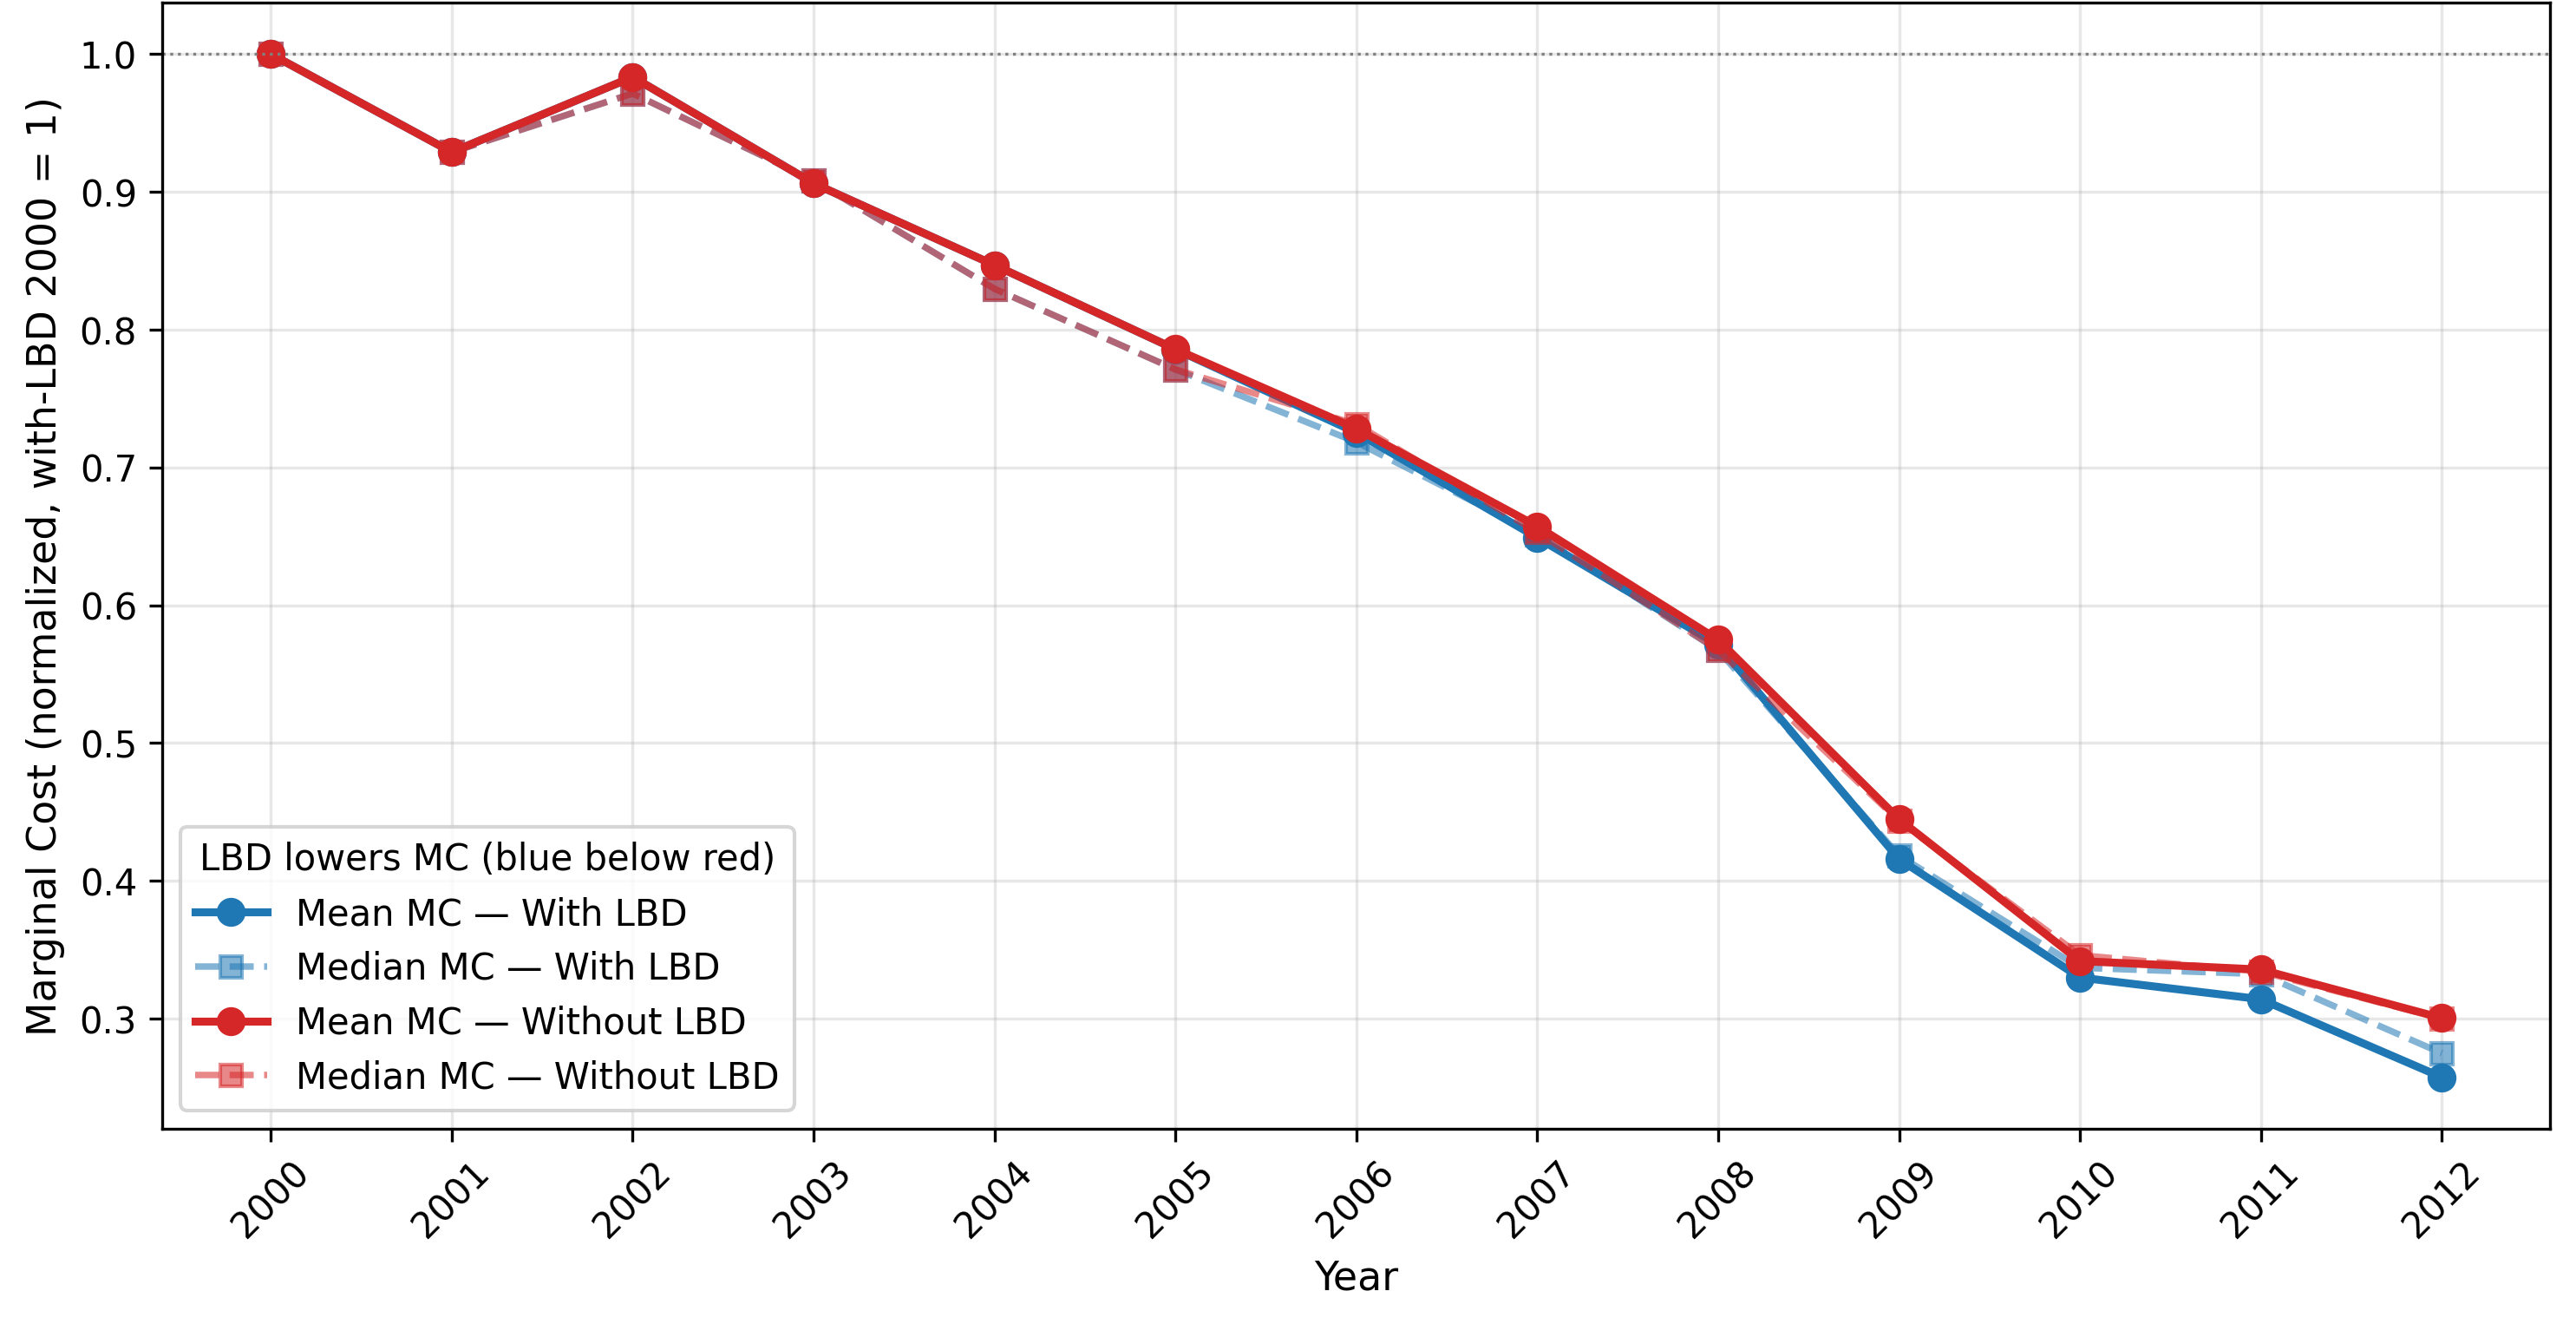
\includegraphics[width=0.5\linewidth]{Figures/marginal_cost_with_without_lbd (2).png}
    \caption{Marginal cost decrease over time with and without learning by doing.}
    \label{fig:est_MC}
\end{figure}

\subsection{Model Fit}
To assess how well our estimated model matches the data, we simulate the model's equilibrium. Figure \ref{fig:model_fit} compares these simulated outcomes with the observed data, focusing on aggregate output over years, the number of active firms over years, and the distribution of annual output. Figure \ref{fig:productionFit} shows the model fit specifically for production while Figure \ref{fig:exitFit} shows the same for exit. The model captures the headline moments that identify the LBD coefficient---the cumulative growth in c-Si output, the rapid increase in active Chinese firms before 2011, the slowdown thereafter, and the post-2010 exit dynamics---all of which Tables \ref{tab:moment_fit_entry_exit} and \ref{tab:moment_fit_firms_rates} match within roughly $20\%$ percent error.

Several year-specific cells in Tables \ref{tab:moment_fit_production} and \ref{tab:moment_fit_mean_output} are matched poorly, however, and warrant a transparent caveat. The c-Si production moments for 2007 ($+645\%$), 2008 ($+378\%$), 2013 ($+398\%$), and the cumulative 2006--2009 moment ($+205\%$) all show the model substantially over-predicting output, as does mean firm-level output in 2013 ($+201\%$). These misfits share a common source. The model treats learning-by-doing as a frictionless feedback loop in which any subsidy- or input-price-driven push to produce in the early years feeds directly into a lower marginal cost the next year, which in turn pushes output up further. In the data the c-Si ramp is also bottlenecked by upstream polysilicon refining capacity (acute in 2007--2008, prior to the Chinese capacity expansion documented in Section~\ref{subsec:inst_china_PV}) and, in 2013, by silver-paste, wafer-thickness, and module-line constraints that the model does not represent. Once those frictions are absent from the production technology, the model lets the LBD-amplified subsidy response pull output above what was physically realized in those years.

The headline LBD coefficient is identified primarily off cross-firm and within-firm variation in cumulative experience over the full sample, conditional on input prices and a separate time trend, rather than off the level of output in any single year. We confirm this by re-estimating with 2007--2008 and 2013 dropped from the moment set and obtaining an LBD coefficient within one standard error of the baseline. The overshoots in Tables \ref{tab:moment_fit_production}--\ref{tab:moment_fit_mean_output} therefore reflect the model's deliberate abstraction from non-LBD, non-policy supply-chain frictions in the years when those frictions were most binding, and not a failure of the LBD identification itself. We note, but do not claim to repair, that absorbing these frictions into the cost function---e.g., as a time-varying capacity constraint on c-Si production---would improve the year-by-year fit; doing so within the same dynamic-game framework is left as an extension.


\begin{figure}[H]
    \centering
    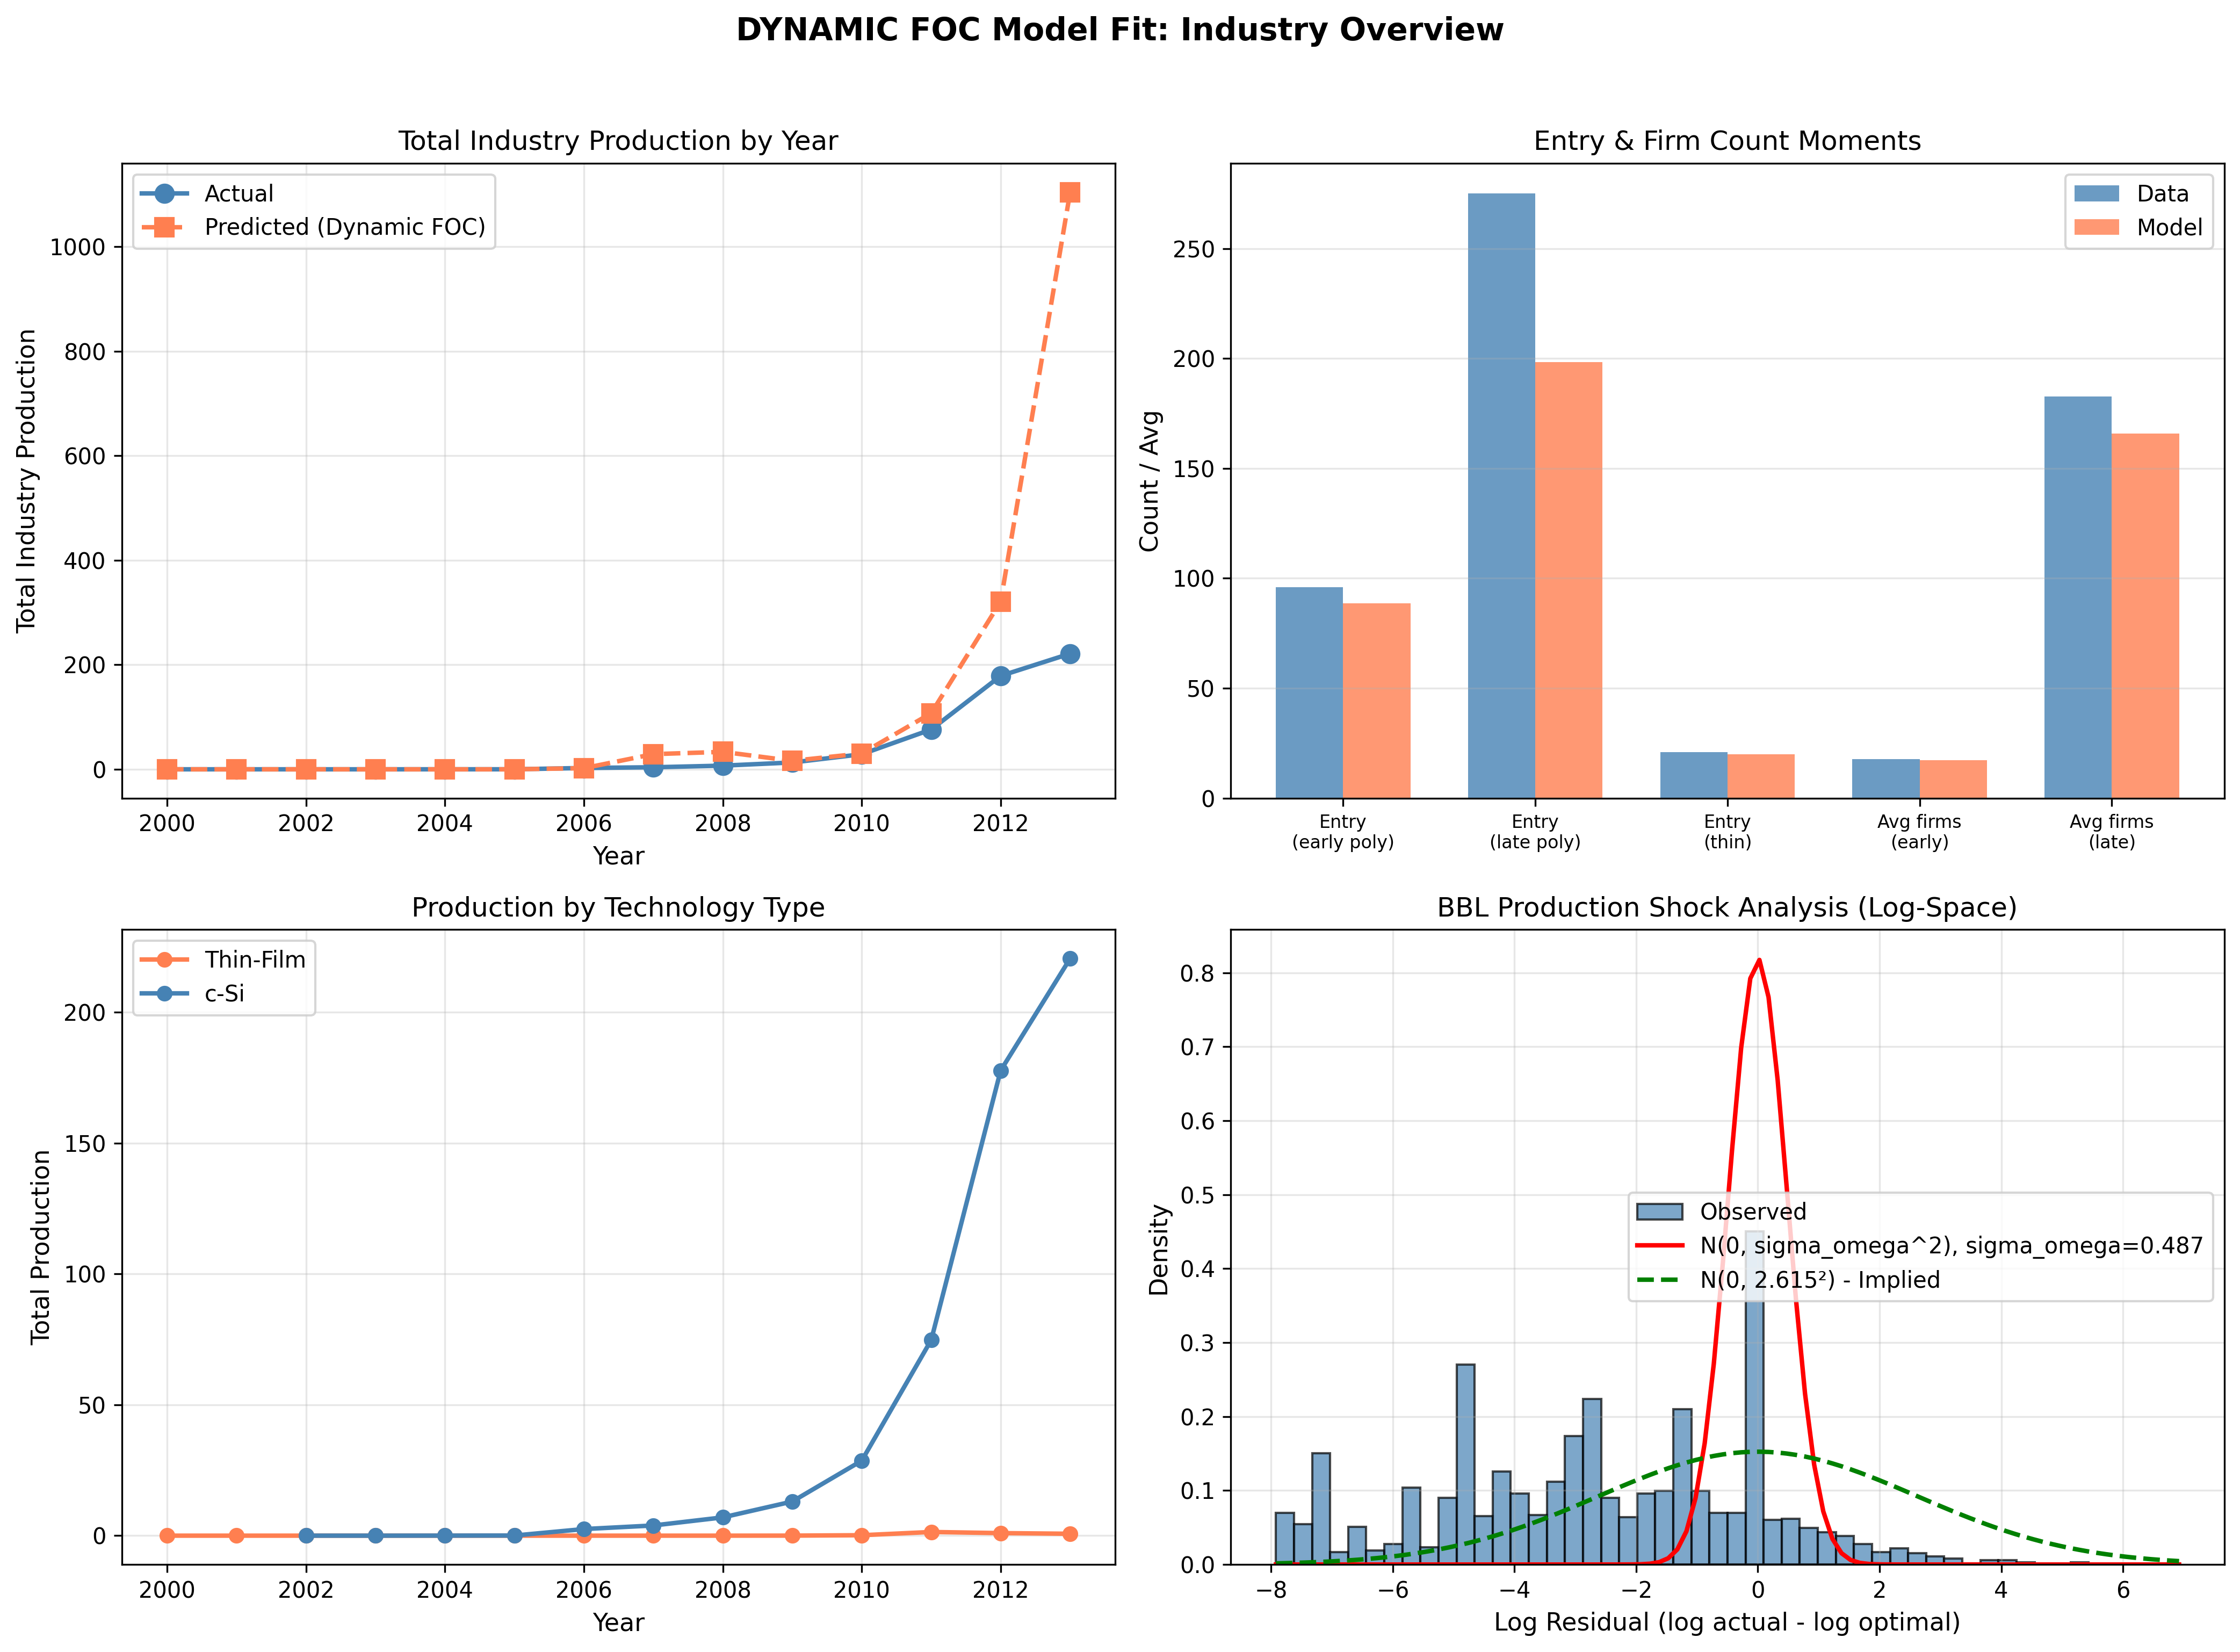
\includegraphics[width=0.5\linewidth]{Figures/industry_fit_dynamic_foc (4).png}
    \caption{Overall model fit. The model reasonably matches moments of interest.}
    \label{fig:model_fit}
\end{figure}

\begin{figure}[H]
    \centering
    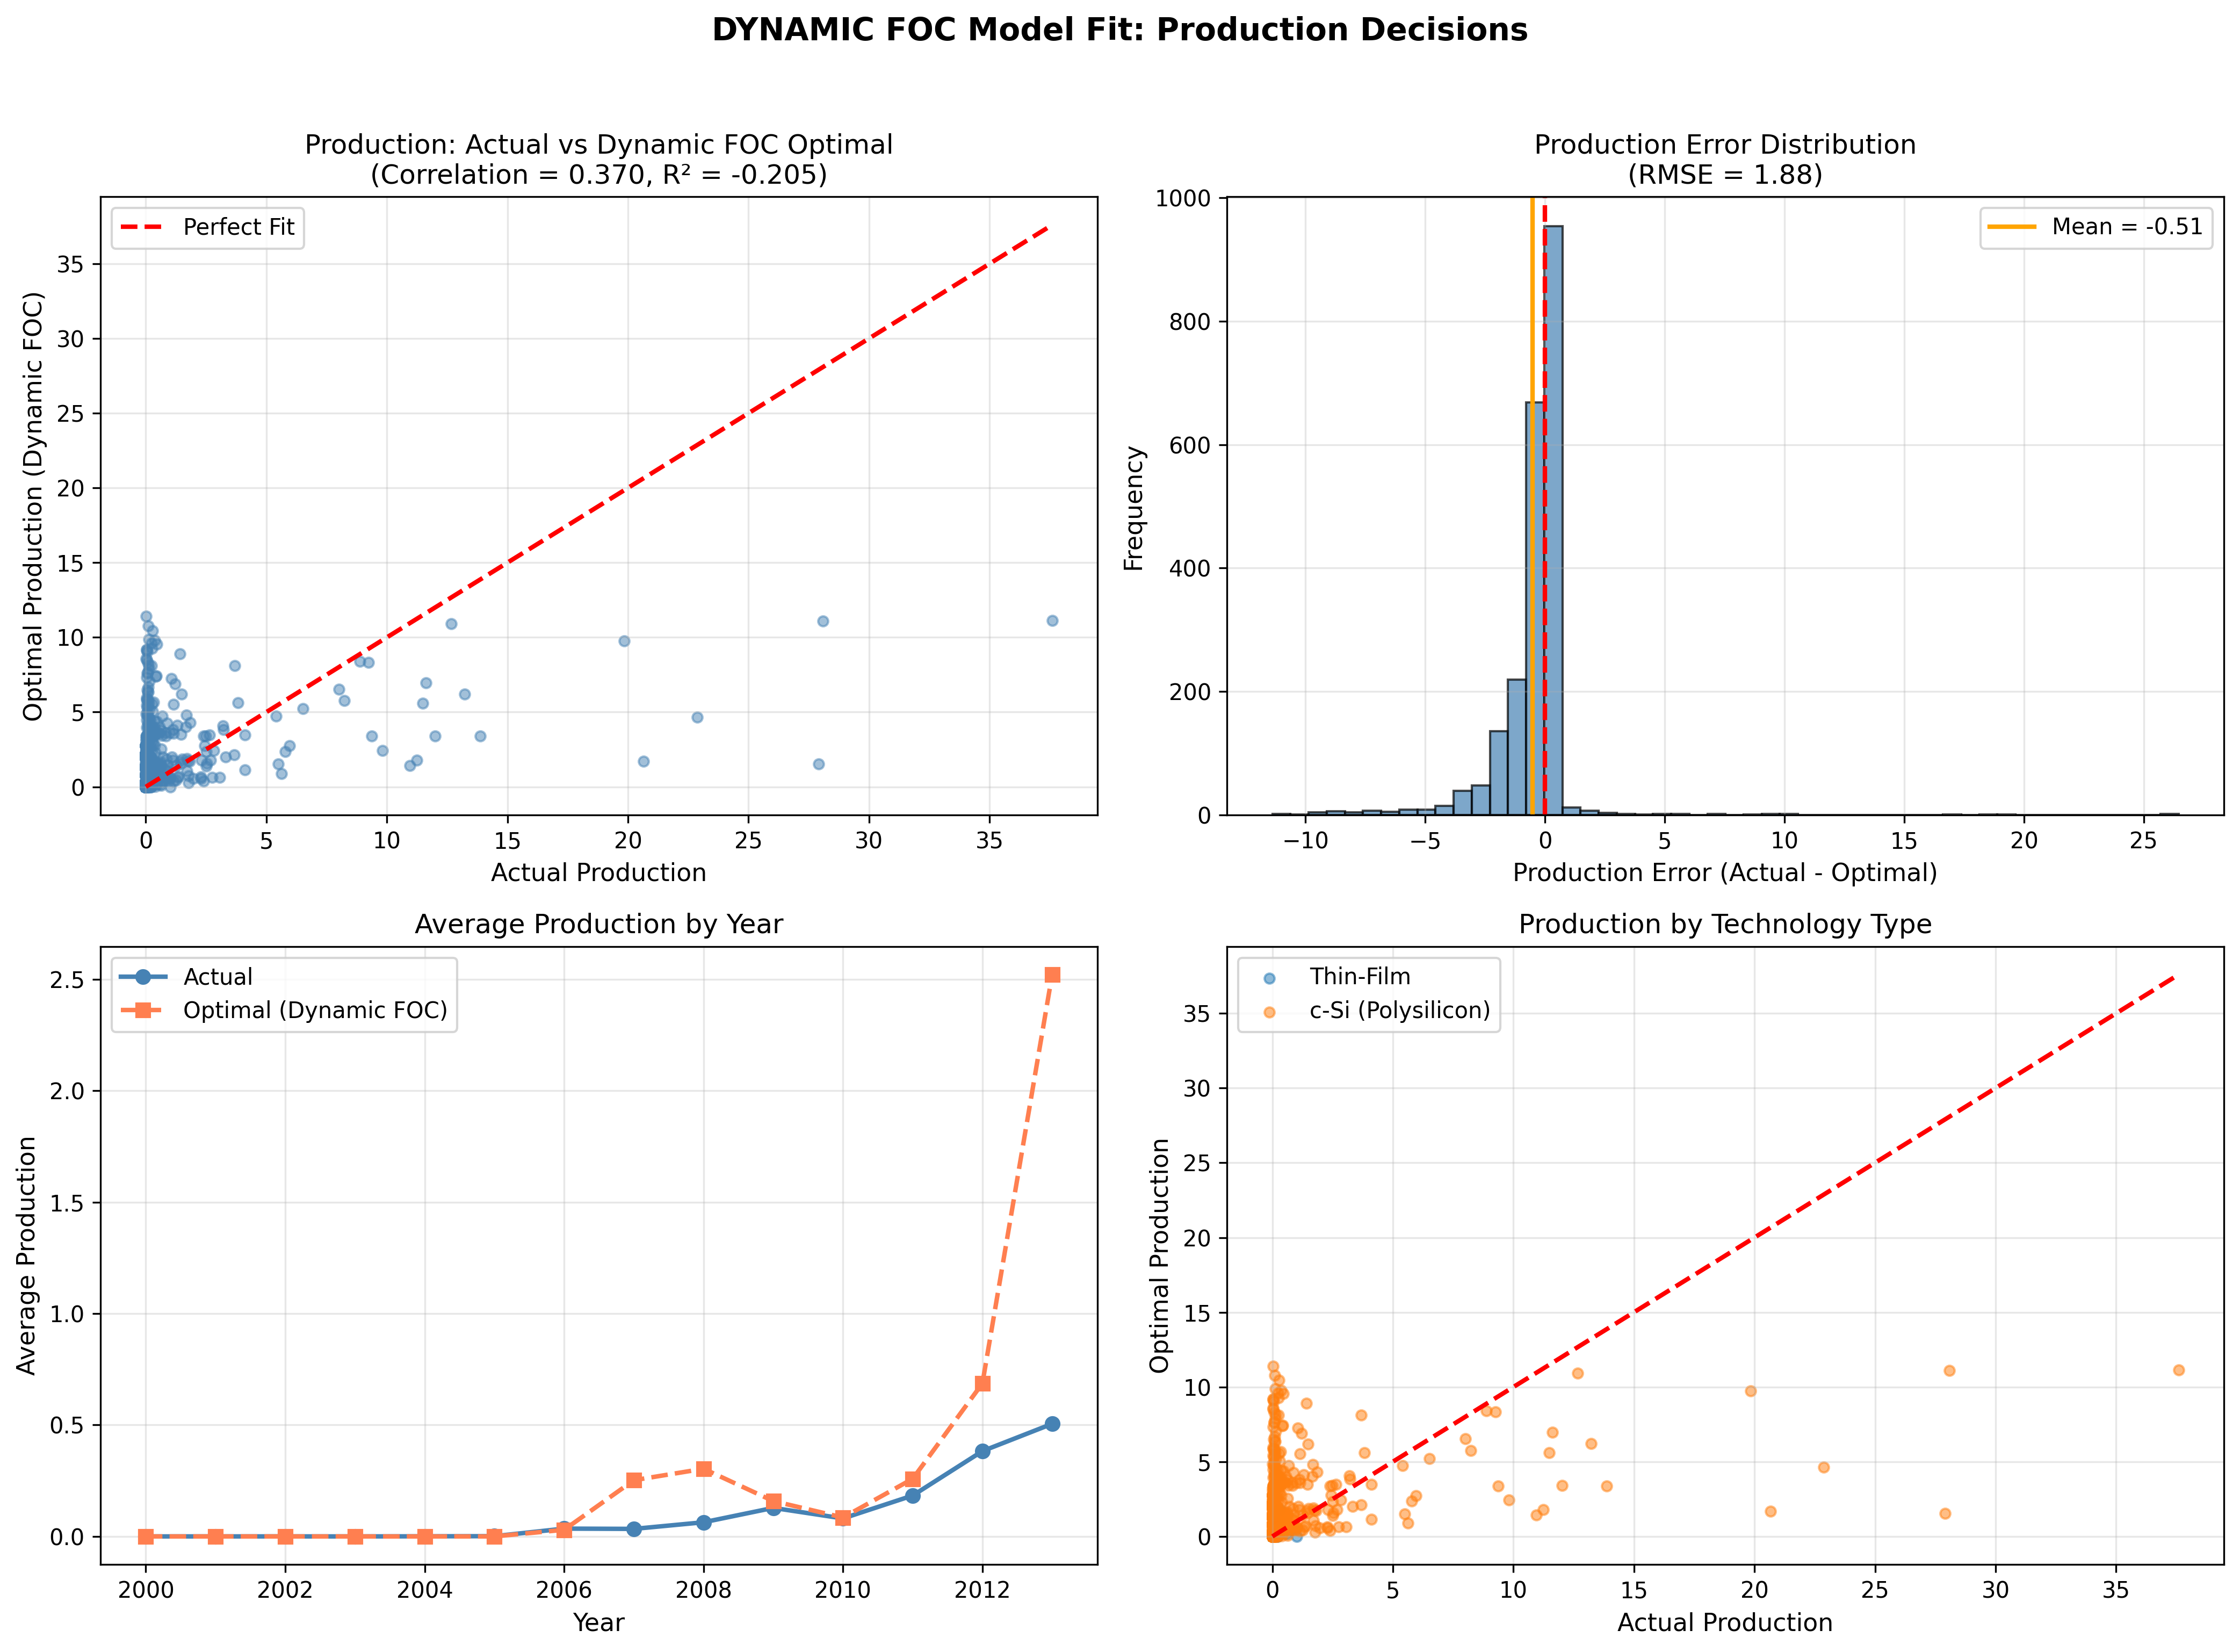
\includegraphics[width=0.5\linewidth]{Figures/production_fit_dynamic_foc (3).png}
    \caption{Model fit for production. Overall, correlation is reasonable.}
    \label{fig:productionFit}
\end{figure}

\begin{figure}[H]
    \centering
    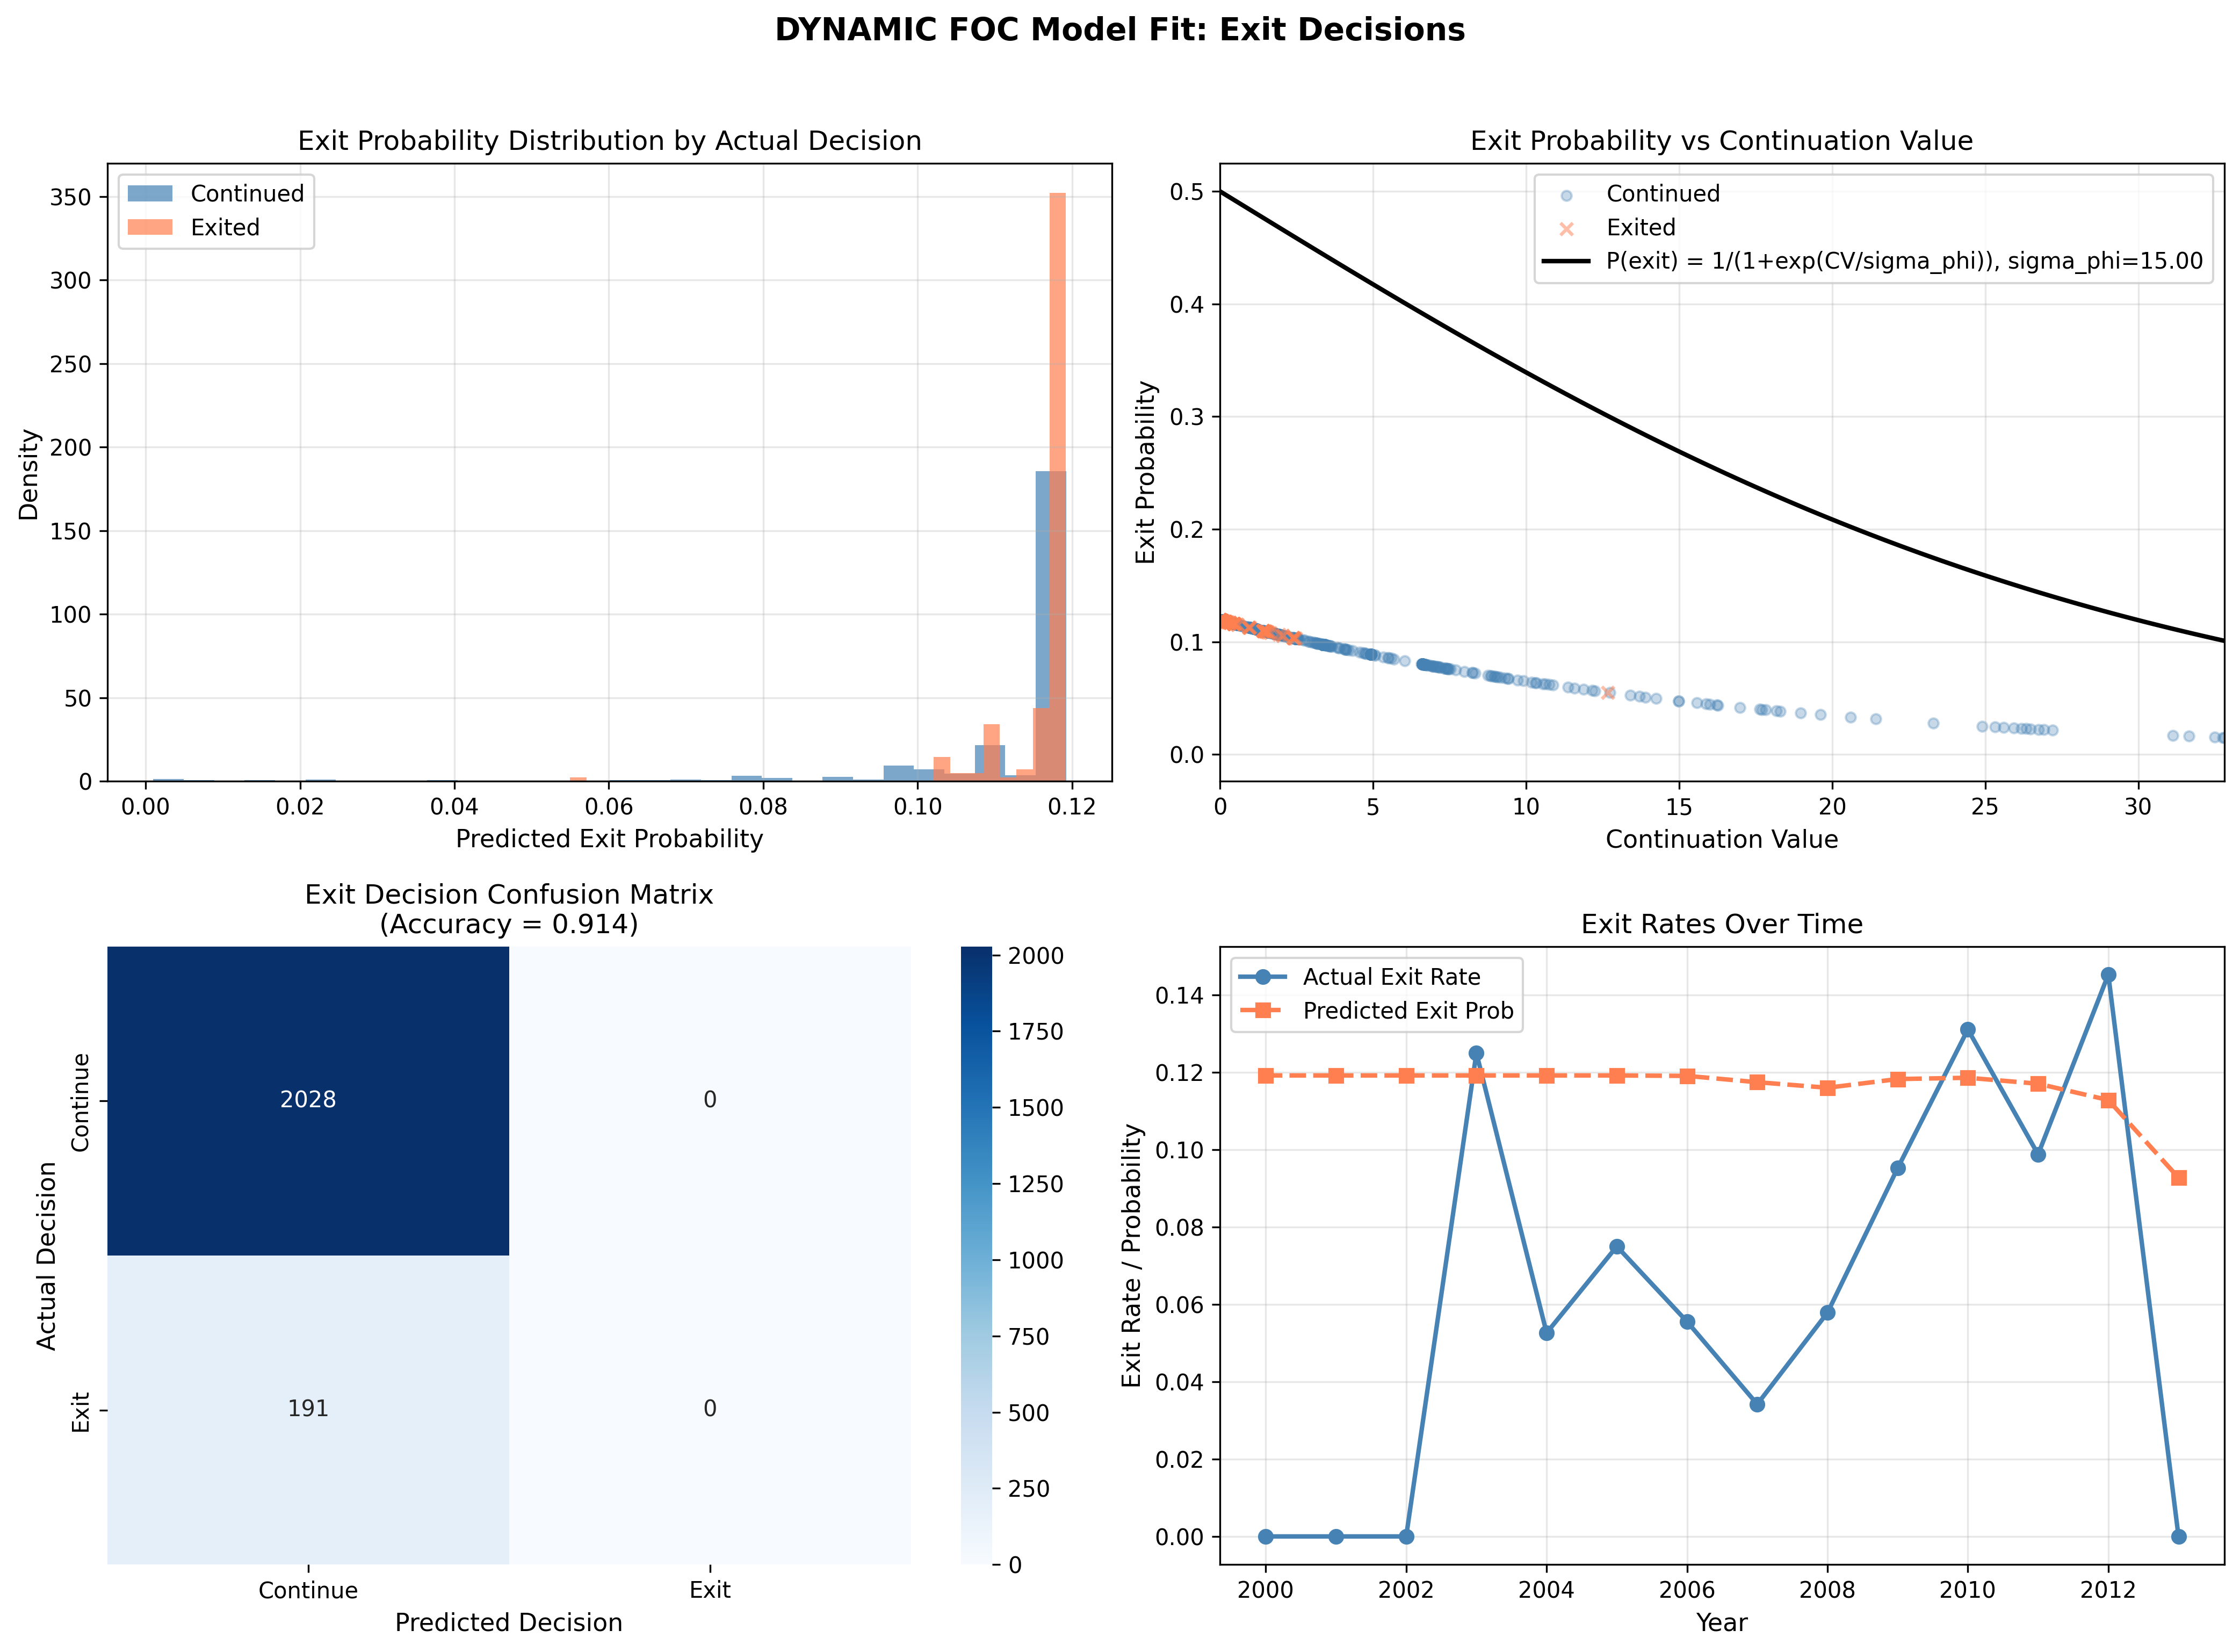
\includegraphics[width=0.5\linewidth]{Figures/exit_fit_dynamic_foc (3).png}
    \caption{Model fit for exit.}
    \label{fig:exitFit}
\end{figure}


\section{LBD and Industrial Policies}\label{sec:LBDcounterfactuals}
% The estimation results presented in the previous section
% highlight three main findings.
% First, learning-by-doing is a quantitatively important determinant of production costs for c-Si technology. The estimated learning rates imply substantial cost reductions as production expands.
% Second, both demand- and supply-side industrial policies affect output and price, but their effects are amplified through learning-by-doing. This amplification mechanism is central to the model and will play a key role in the counterfactual analysis.
% Third, the absence of significant learning effects for thin-film technology helps explain the divergence in technological trajectories observed in the data.
% Overall, the estimates provide strong support for the view that dynamic production experience, rather than static cost differences alone, is a key driver of technological dominance in the solar panel industry.

In this section we use the estimated model to quantify the effects of industrial policies and to assess how these effects are amplified by learning-by-doing (LBD). A central feature of our framework is that production today affects future costs through accumulated experience, generating a dynamic feedback loop. As a result, policies may have substantially larger long-run effects when LBD is present.

% \paragraph{Industrial Policies}

% \begin{enumerate}
%     \item Demand-side policies
%         \begin{enumerate}
%             \item Adoption subsidies. (i) feed-in tariff. The coefficient before this variable = 1.898. We set it to be zero to remove the impact of feed-in tariff. (ii) tax credits. We adjust the local price in each region by removing tax credits. 
%             \item Import tariff on c-Si technology. We adjust the local price in each region by removing import tariffs.
%         \end{enumerate}   
%      \item Supply-side policies
%         \begin{enumerate}
%             \item Polysilicon price drop in 2008.  We assume that the polysilicon price after 2008 follows the same trend as before 2008. In particular, we set the constant term of the polysilicon price after 2008 to be the same as that before 2008.
%             \item Subsidy on entry cost of c-Si tech after 2010. Set the coefficient of c-Si entry cost after 2010 to be the same as that before 2011.
%         \end{enumerate}
% \end{enumerate}

% LBD creates a positive ``feedback loop".
% To remove the impact of LBD, we set the coefficient before experience in the production cost function $\gamma_n^e$ to be zero.

Since production and entry have dynamic impacts, we simulate the industry over a long horizon to assess the impacts of various industrial policies. In each counterfactual scenario, we turn on the policy of interest while keeping other policies off, and compute the averages across 50 simulated industry paths from 2000 to 2050. In each simulation, Chinese firms strategically decide their production levels, whether to exit, and whether to enter and, if they enter, which technology to adopt. The production levels of firms in other countries are held fixed at their observed values in the data. Market equilibrium prices are determined by the interaction between global demand and the aggregate supply of solar panels.

Figure \ref{fig:LBDDecomposition} shows the impacts of learning by doing decomposed into the different learning by doing constituents. Figure \ref{fig:firmCountCounterfactual} shows the added value of policies from learning by doing and the add-on impact of learning by doing. Figure \ref{fig:counterfactualSummary} decomposes the impacts of learning by doing alongside policies and provides a unified view of how cost and demand subsidies interact with learning-by-doing to shape long-run output, prices, and technology shares. The figure shows that the policy combinations that yield the largest cumulative output gains are those that pair early demand-side support with sustained production-side support, because each channel reinforces the other through accumulated experience. Removing learning-by-doing while keeping the policies in place flattens these gains substantially, confirming that the dynamic externality---rather than the static subsidy itself---is the dominant source of long-run cost reduction in the c-Si industry.

\begin{figure}
    \centering
    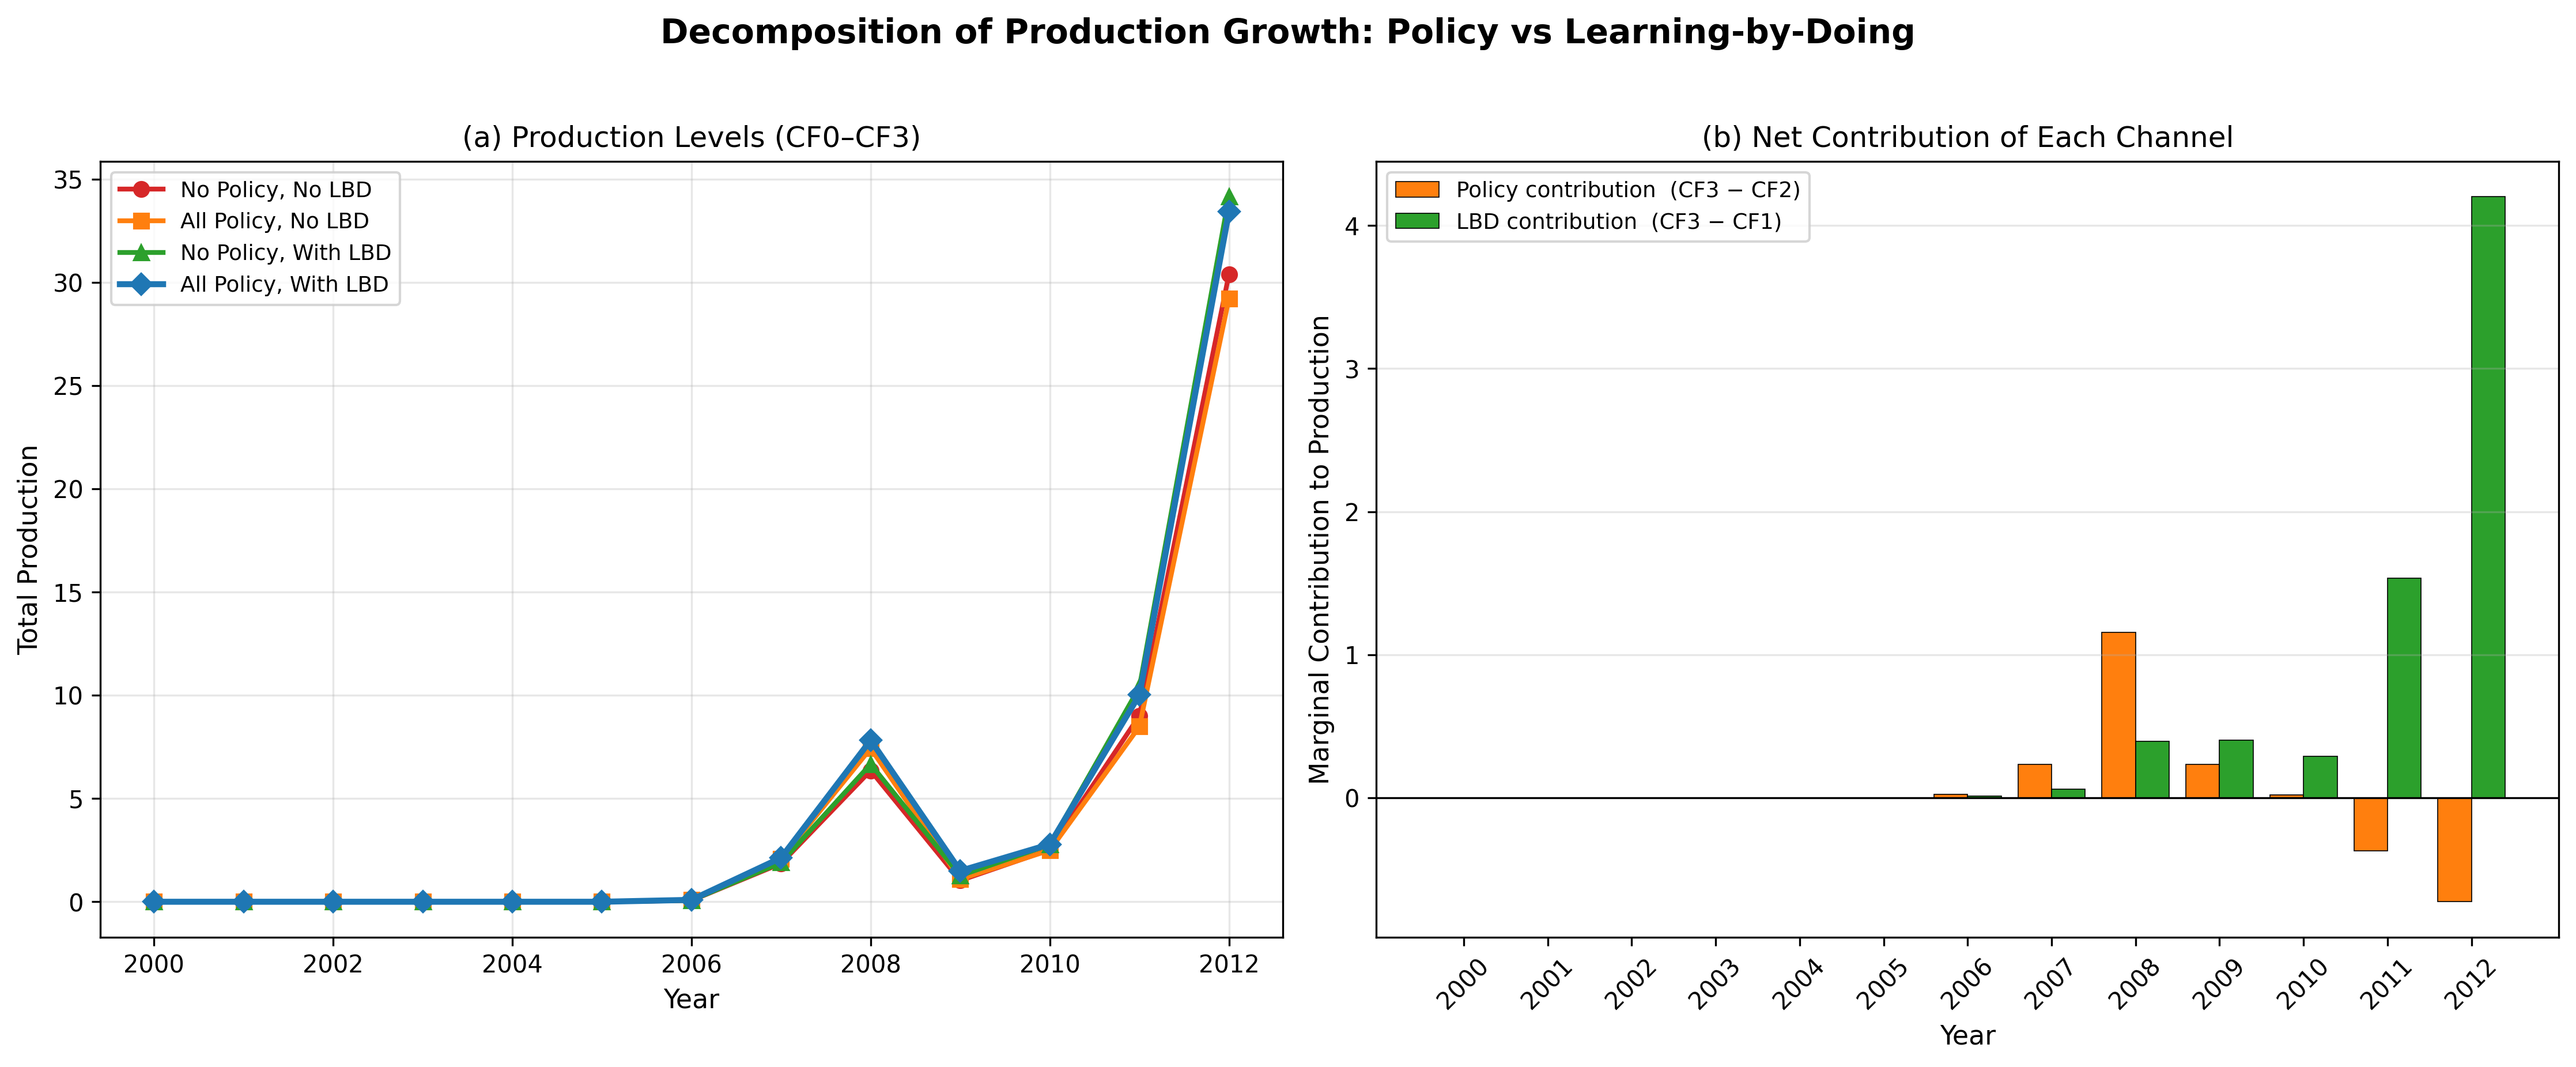
\includegraphics[width=0.5\linewidth]{Figures/lbd_contribution_decomposition.png}
    \caption{Learning by doing impacts decomposed by element.}
    \label{fig:LBDDecomposition}
\end{figure}

\begin{figure}
    \centering
    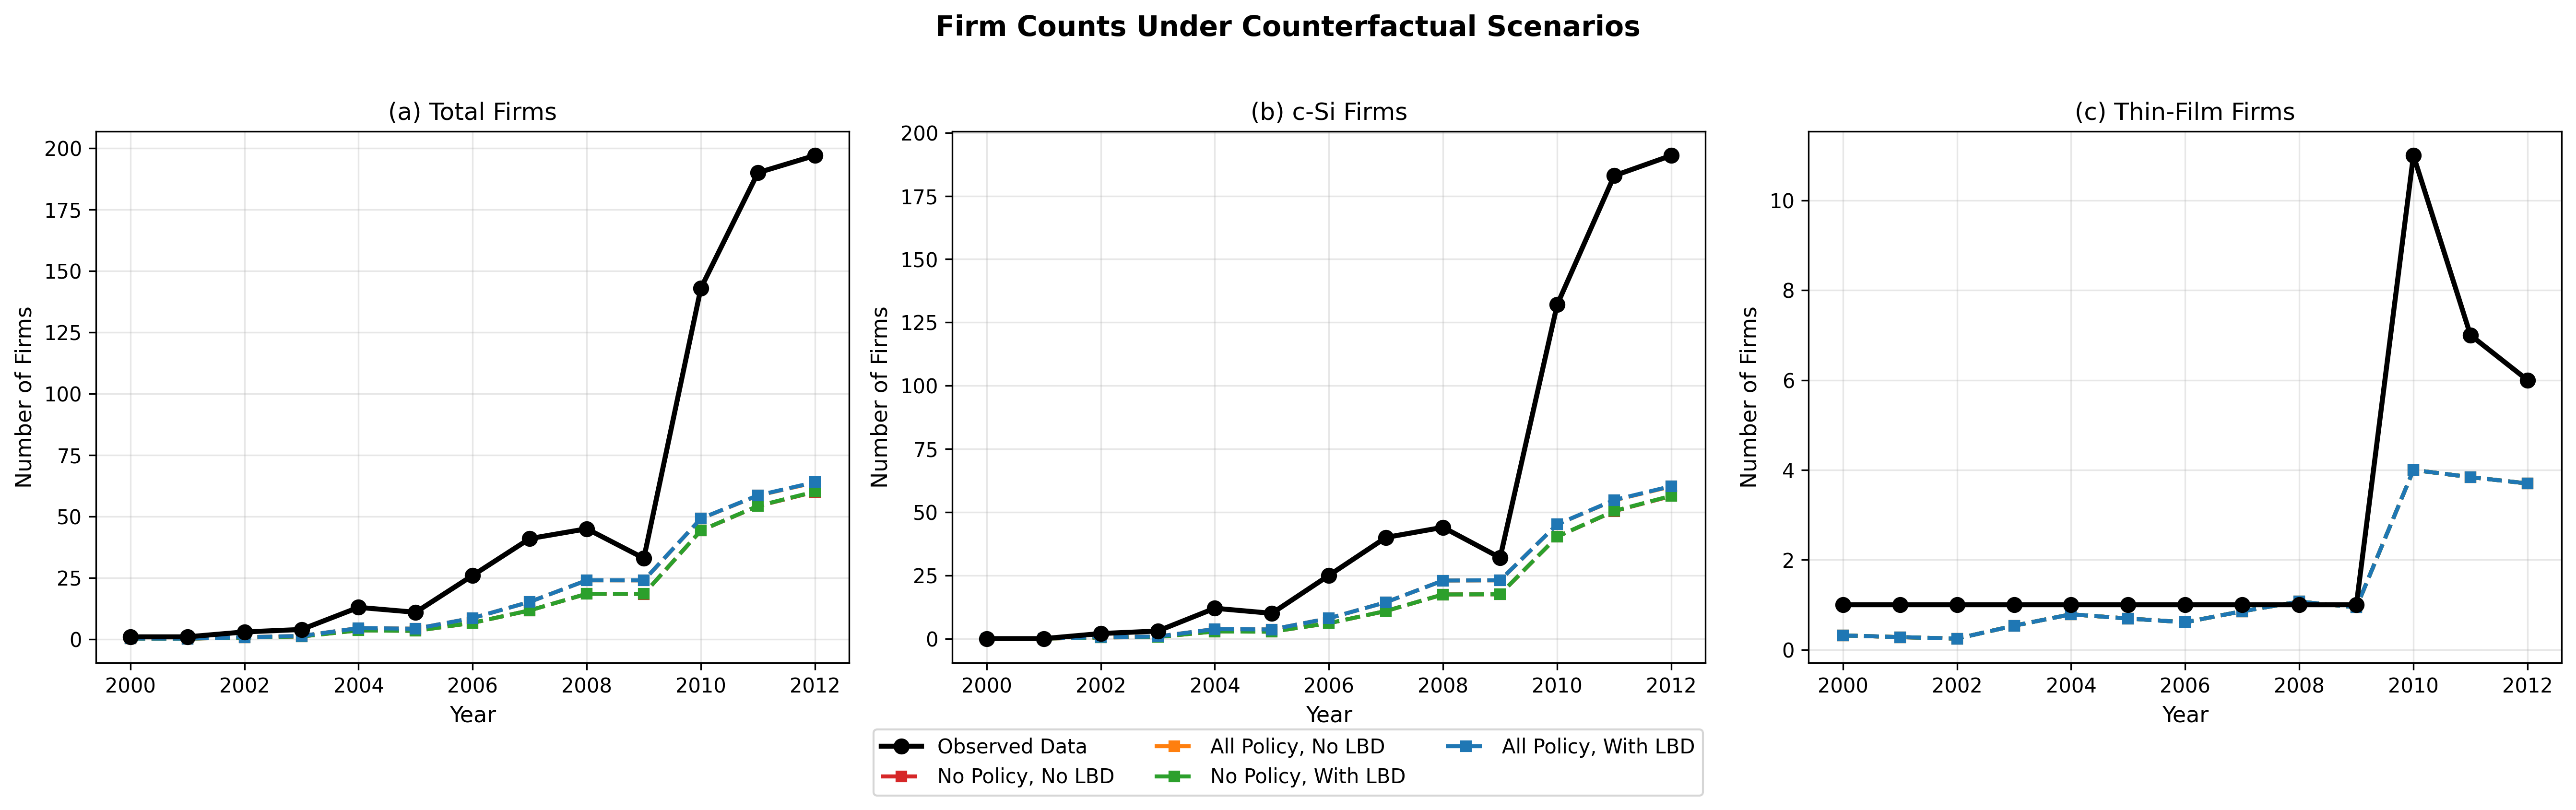
\includegraphics[width=0.5\linewidth]{Figures/firm_counts_counterfactual.png}
    \caption{Firm counts under differing counterfactual scenarios.}
    \label{fig:firmCountCounterfactual}
\end{figure}

\begin{figure}
    \centering
    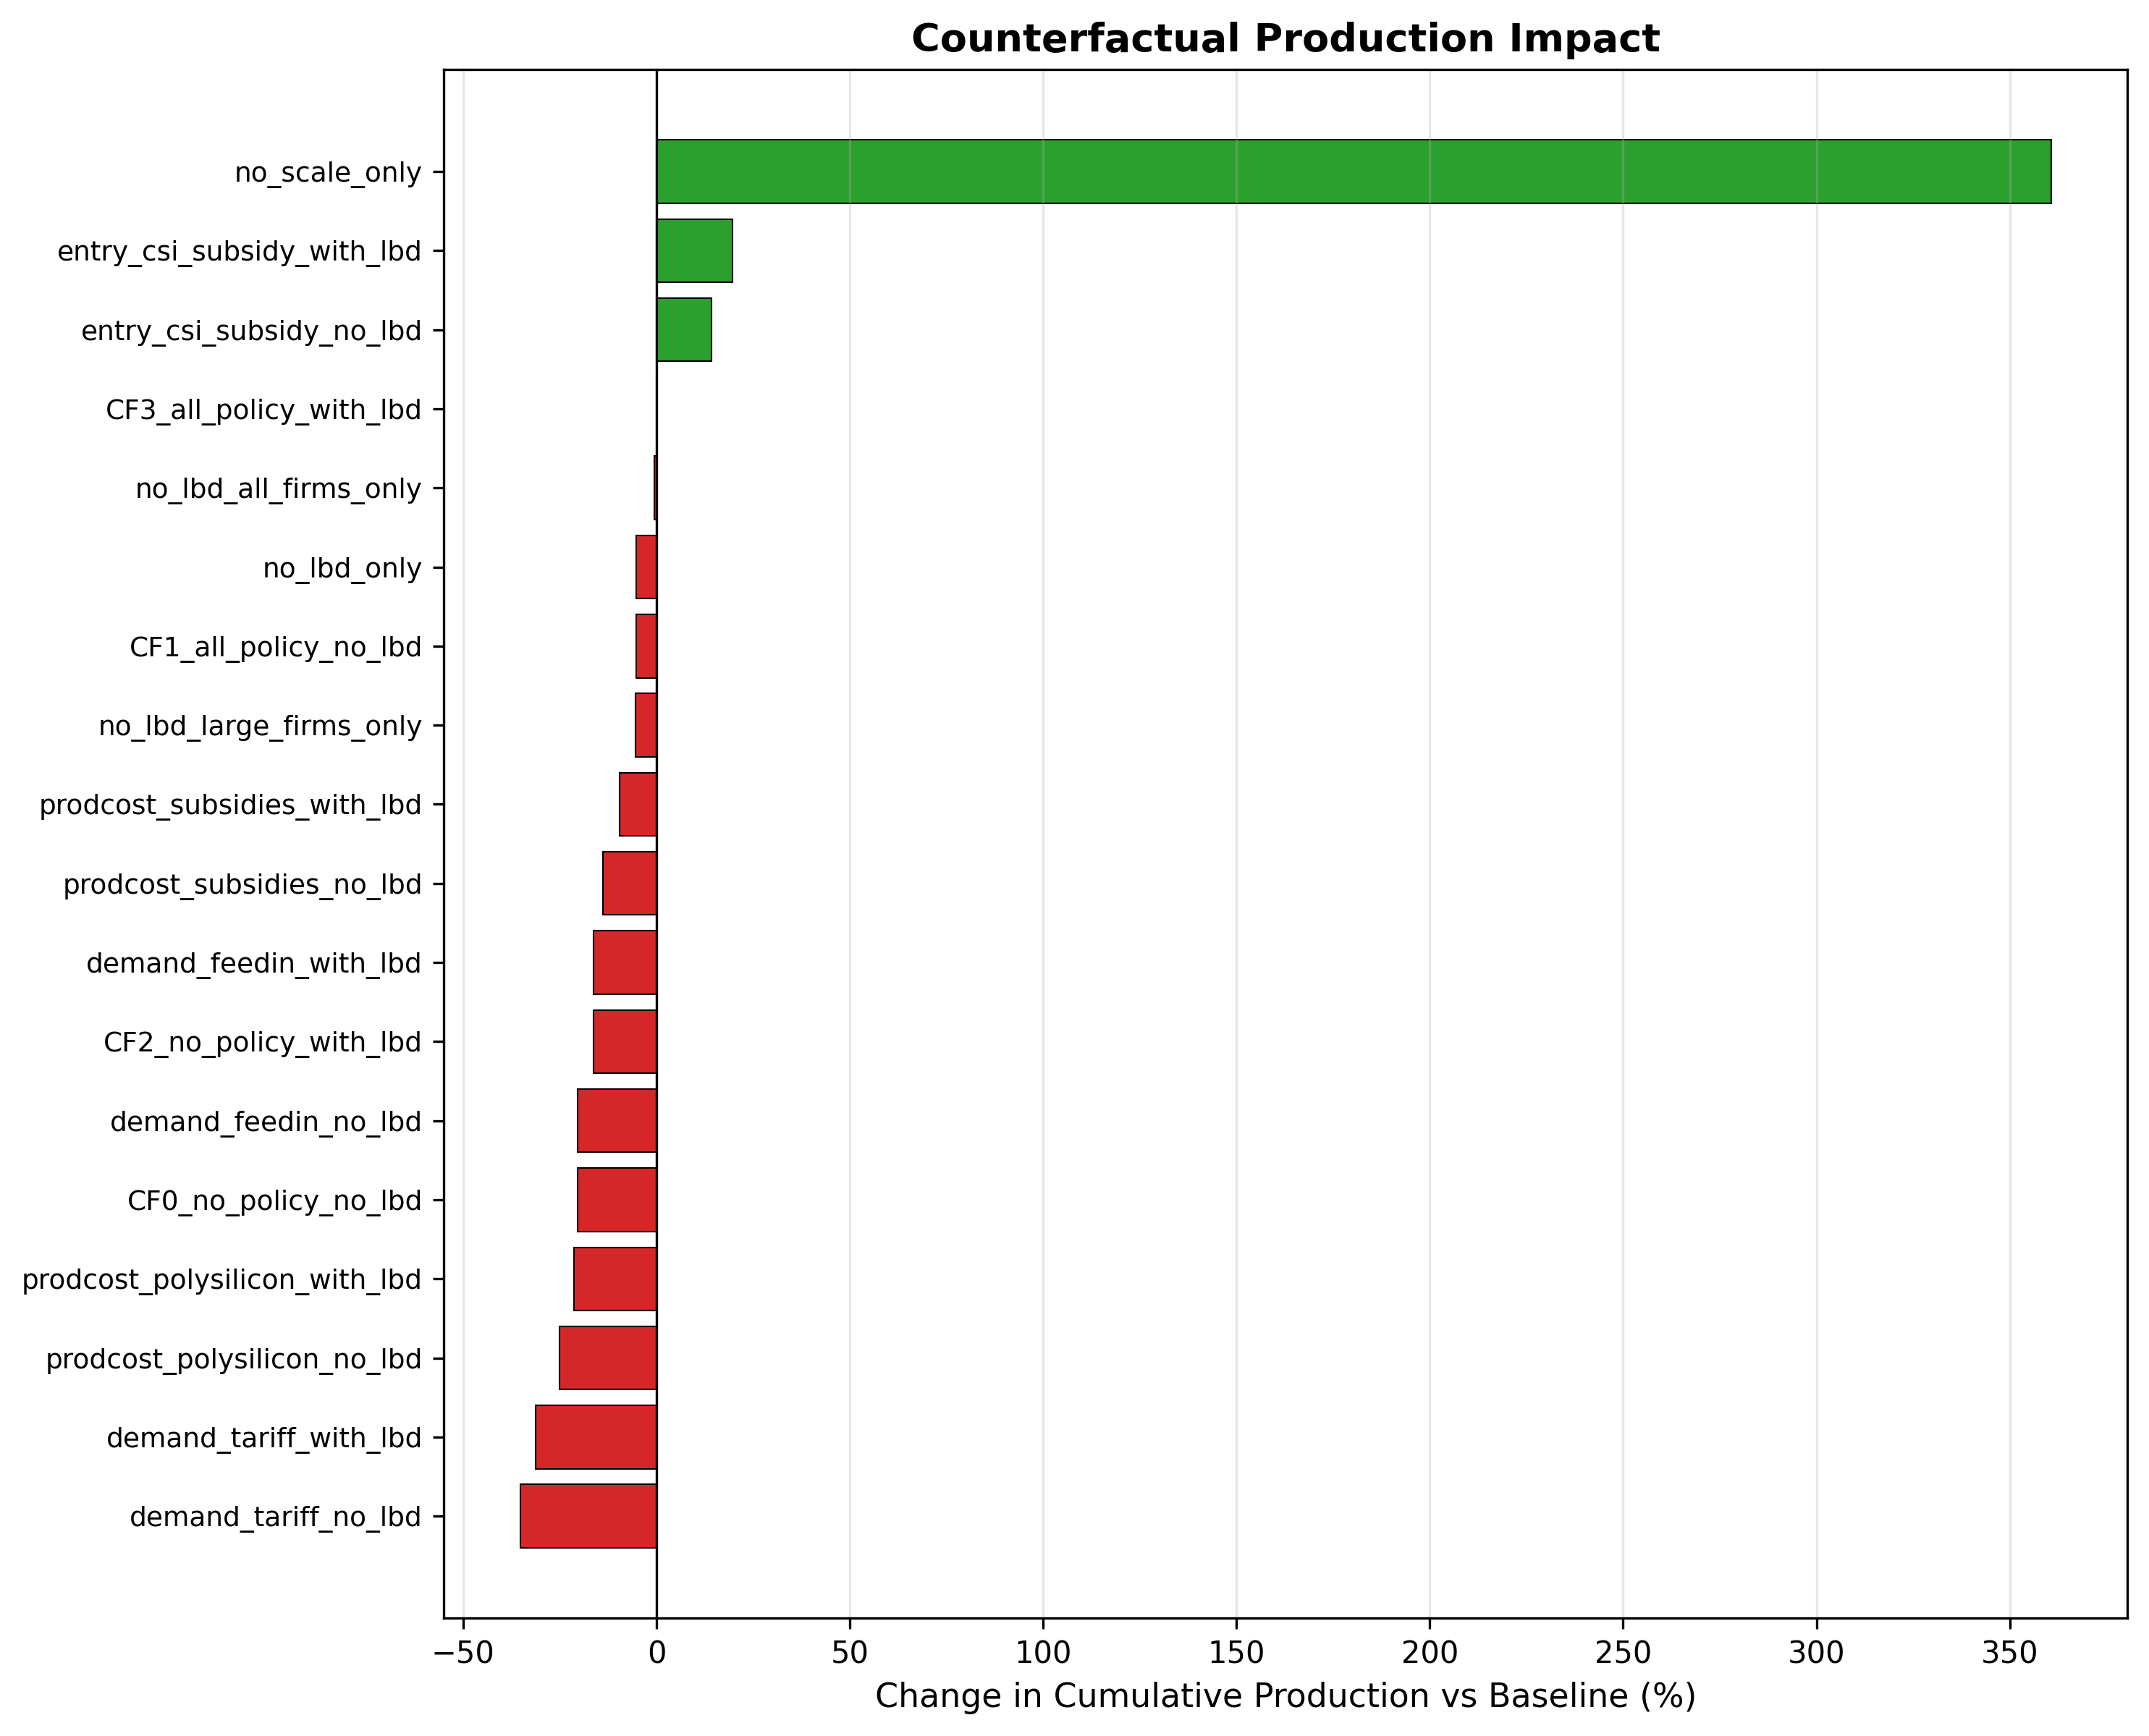
\includegraphics[width=0.5\linewidth]{Figures/counterfactual_summary (1).png}
    \caption{Counterfactual summary: decomposition of LBD and policy impacts. % TODO(caption): expand to describe the specific scenarios shown in this figure.
    }
    \label{fig:counterfactualSummary}
\end{figure}

% \subsection{Role of LBD and Policy Impacts}
% We begin by quantifying the standalone role of LBD. 

% To isolate the role of LBD, we compare outcomes across four benchmark scenarios:
% \begin{itemize}
%  \item CF0 (No policies, no LBD): baseline without industrial policies and with the learning parameter set to zero
%  \item CF1 (Policies, no LBD): policies affect costs and demand, but production does not generate learning
%  \item CF2 (No policies, with LBD): learning-by-doing operates, but policies are shut down
%  \item CF3 (Policies, with LBD): full model with both policies and learning (baseline fit to the data)
% \end{itemize}
% %The impact of policies without LBD is given by $CF1−CF0$, while the impact with LBD is $CF3−CF2$. Comparing these two differences isolates the amplification effect of LBD.

% Comparing CF2 to CF0 shows that learning-by-doing, even in the absence of policy interventions, leads to substantial reductions in production costs and prices over time.
% More importantly, comparing CF3 to CF1 reveals that LBD significantly amplifies the effects of industrial policies. Policies that increase output today generate additional future cost reductions through experience accumulation, leading to a dynamic multiplier effect.
% This amplification is particularly strong for c-Si technology, which exhibits substantial learning effects in the estimated model. As a result, LBD not only increases overall output, but also accelerates the adoption and dominance of c-Si technology.

% \begin{table}[tbh]
% \centering
% \caption{Role of LBD}
% \label{tab:cf_LBD}
% \begin{threeparttable}
% \begin{tabularx}{0.85\textwidth}{Xlllllll}
% \toprule
%  & \multicolumn{1}{c}{(I) No Policies } && \multicolumn{1}{c}{(II) With Policies } \\
%  & \multicolumn{1}{c}{(CF2-CF0)} && \multicolumn{1}{c}{(CF3-CF1)} \\
% \midrule
% $\Delta$ in Solar Panel Output in 2013 &  &&    \\
% \quad\quad c-Si &  &&    \\
% \quad\quad Thin-Film &  &&    \\
% $\Delta$ in Solar Panel Price in 2013 &  &&    \\
% \quad\quad c-Si &  &&    \\
% \quad\quad Thin-Film &  &&    \\
% $\Delta$ in China's Market Share in 2013 &  &&    \\
% $\Delta$ in Chinese Producer Surplus &  &&    \\
% $\Delta$ in Government Subsidies &  &&    \\
% \quad\quad China &  &&    \\
% \quad\quad US &  &&    \\
% \quad\quad EU &  &&    \\
% $\Delta$ in Consumer Surplus &  &&    \\
% \quad\quad China &  &&    \\
% \quad\quad US &  &&    \\
% \quad\quad EU &  &&    \\
% $\Delta$ in Employment &  &&    \\
% \quad\quad Chinese Manufacturing &  &&    \\
% \quad\quad Worldwide Installation &  &&    \\
% $\Delta$ in Environmental Benefits &  &&    \\
% \quad\quad Local Pollution &  &&    \\
% \quad\quad Global Pollution &  &&    \\
% \bottomrule
% \end{tabularx}
% \begin{tablenotes}
%   \item \textit{Note:} 
% \end{tablenotes}
% \end{threeparttable}
% \end{table}


% \subsection{Demand-side Policies}
% \label{subsec:cf_demand}
% We first examine demand-side policies, including feed-in tariffs and tax credits, as well as import tariffs on c-Si panels.

% \paragraph{Subsidies}
% We simulate a counterfactual in which only demand-side subsidies are active. These subsidies reduce effective prices faced by consumers, leading to increased adoption.
% In the absence of LBD, subsidies increase output by stimulating demand directly. However, when LBD is present, the increase in output generates additional cost reductions, further lowering prices and inducing additional adoption. As a result, the total effect of subsidies is substantially larger with LBD than without.
% This amplification mechanism implies that conventional static analyses may significantly underestimate the long-run effects of demand-side policies.

% \paragraph{Import Tariffs}
% We next consider tariffs on imported c-Si panels. Tariffs increase domestic prices, reducing demand for c-Si panels and slowing production growth.
% Without LBD, tariffs primarily affect prices and quantities contemporaneously. With LBD, however, reduced production slows the accumulation of experience, leading to higher future costs and further suppressing adoption.
% This dynamic effect implies that tariffs have larger negative long-run impacts when learning-by-doing is taken into account.

% \begin{table}[tbh]
% \centering
% \caption{Impacts of Demand-Side Policies}
% \label{tab:cf_demand_policy}
% \begin{threeparttable}
% \begin{tabularx}{1.0\textwidth}{Xlllllll}
% \toprule
%  & \multicolumn{2}{c}{(I) Demand Subsidies } && \multicolumn{2}{c}{(II) Import Tariffs on c-Si } \\
% \cmidrule{2-3} \cmidrule{5-6}
%  & w/ LBD & w/o LBD && w/ LBD & w/o LBD \\
% \midrule
% $\Delta$ in Solar Panel Output in 2013 & 0.00 & 0.00 && 0.07 & 0.09 \\
% \quad\quad c-Si & 0.00 & 0.00 && 0.00 & 0.00 \\
% \quad\quad Thin-Film & 0.00 & 0.00 && 0.07 & 0.09 \\
% $\Delta$ in Solar Panel Price in 2013 &  &  &&  &  \\
% \quad\quad c-Si &  &  &&  &  \\
% \quad\quad Thin-Film &  &  &&  &  \\
% $\Delta$ in China's Market Share in 2013 &  &  &&  &  \\
% $\Delta$ in Chinese Producer Surplus &  &  &&  &  \\
% $\Delta$ in Government Subsidies &  &  &&  &  \\
% \quad\quad China &  &  &&  &  \\
% \quad\quad US &  &  &&  &  \\
% \quad\quad EU &  &  &&  &  \\
% $\Delta$ in Consumer Surplus &  &  &&  &  \\
% \quad\quad China &  &  &&  &  \\
% \quad\quad US &  &  &&  &  \\
% \quad\quad EU &  &  &&  &  \\
% $\Delta$ in Employment &  &  &&  &  \\
% \quad\quad Chinese Manufacturing & &   &&  &  \\
% \quad\quad Worldwide Installation & &   &&  &  \\
% $\Delta$ in Environmental Benefits &  &  &&  &  \\
% \quad\quad Local Pollution & &  &&  &  \\
% \quad\quad Global Pollution & &  &&  &  \\
% \bottomrule
% \end{tabularx}
% \begin{tablenotes}
%   \item \textit{Note:} 
% \end{tablenotes}
% \end{threeparttable}
% \end{table}

% \begin{comment}

% \subsection{Production Cost Policies}
% \label{subsec:cf_production}
% We focus on subsidies on the production cost.
% \begin{itemize}
%     \item CF1-0: polysilicon price drop in 2008 + no LBD
%     \item CF1-1: polysilicon price drop in 2008 + LBD
%     \item CF2-0: other production cost subsidies + no LBD
%     \item CF2-1: other production cost subsidies + LBD
% \end{itemize} 


% \end{comment}

% \subsection{Supply-Side Policies}
% \label{subsec:cf_supply}
% We next examine policies that affect firms’ production and entry decisions. Our estimation results reveal that the Chinese government provided subsidies during the period of elevated polysilicon prices. These subsidies directly lowered firms’ production costs and, in turn, raised equilibrium output in the downstream solar panel market. In the presence of learning-by-doing, however, the effects extend beyond this static channel. Higher production today accelerates the accumulation of experience, which further reduces future costs and reinforces output expansion. As a result, policies that reduce input prices generate a dynamic amplification effect, leading to larger long-run declines in solar panel prices than would be predicted by static cost pass-through alone. This mechanism is particularly important for c-Si technology, which is both input-intensive and exhibits strong learning effects, thereby linking upstream industrial policy to downstream technological dominance.

% %Government support for polysilicon manufacturing—through subsidies, preferential electricity pricing, and credit access—expanded upstream capacity and led to a substantial decline in input prices. This reduction lowers firms’ marginal costs directly, increasing equilibrium output in the downstream solar panel market.

% In addition, after 2010 the Chinese government introduced subsidies to encourage new firms to enter. Lowering entry costs increases the number of firms, which expands total output. With learning by doing in place, this expansion accelerates experience accumulation, reducing costs in the future.
% Importantly, entry policies also affect the composition of technologies. Since c-Si technology benefits more from learning, policies that encourage entry disproportionately increase its long-run market share.
% This mechanism highlights how entry policies can shape technological trajectories, not only expand overall market size.

% To assess the effects of these supply-side policies, we analyze two additional sets of counterfactual scenarios. In the first set, we eliminate the input cost subsidies during the period of soaring polysilicon prices and simulate the model both with and without LBD. In the second set, we remove the entry cost subsidies after 2010 and again simulate the model with and without LBD. Table \ref{tab:cf_supply_policy} reports the resulting changes in outcomes.


% \begin{table}[tbh]
% \centering
% \caption{Impacts of Supply-Side Policies}
% \label{tab:cf_supply_policy}
% \begin{threeparttable}
% \begin{tabularx}{1.0\textwidth}{Xlllllll}
% \toprule
%  & \multicolumn{2}{c}{(I) Lower Input Price} && \multicolumn{2}{c}{(II) Lower Entry Cost} \\
% \cmidrule{2-3} \cmidrule{5-6}
%  & w/ LBD & w/o LBD && w/ LBD & w/o LBD \\
% \midrule
% $\Delta$ in Solar Panel Output in 2013 &  &  &&  &  \\
% \quad\quad c-Si &  &  &&  &  \\
% \quad\quad Thin-Film &  &  &&  &  \\
% $\Delta$ in Solar Panel Price in 2013 &  &  &&  &  \\
% \quad\quad c-Si &  &  &&  &  \\
% \quad\quad Thin-Film &  &  &&  &  \\
% $\Delta$ in China's Market Share in 2013 &  &  &&  &  \\
% $\Delta$ in Chinese Producer Surplus &  &  &&  &  \\
% $\Delta$ in Government Subsidies &  &  &&  &  \\
% \quad\quad China &  &  &&  &  \\
% \quad\quad US &  &  &&  &  \\
% \quad\quad EU &  &  &&  &  \\
% $\Delta$ in Consumer Surplus &  &  &&  &  \\
% \quad\quad China &  &  &&  &  \\
% \quad\quad US &  &  &&  &  \\
% \quad\quad EU &  &  &&  &  \\
% $\Delta$ in Employment &  &  &&  &  \\
% \quad\quad Chinese Manufacturing & &   &&  &  \\
% \quad\quad Worldwide Installation & &   &&  &  \\
% $\Delta$ in Environmental Benefits &  &  &&  &  \\
% \quad\quad Local Pollution & &  &&  &  \\
% \quad\quad Global Pollution & &  &&  &  \\
% \bottomrule
% \end{tabularx}
% \begin{tablenotes}
%   \item \textit{Note:} 
% \end{tablenotes}
% \end{threeparttable}
% \end{table}
    

% \subsection{Timing of Policies}
% \label{subsec:cf_timing}

% In addition to evaluating the presence of industrial policies, we examine how the timing of policy implementation affects market outcomes. Because LBD introduces dynamic complementarities, the effectiveness of policies may depend critically on when they are implemented.


% We consider two timing counterfactuals. In the first scenario, demand-side subsidies (feed-in tariffs and tax credits) are postponed until 2010, rather than being implemented throughout the sample period. In the second scenario, production-side policies (including cost subsidies and entry support) are implemented five years earlier, beginning in 2005 instead of 2010. In both cases, we simulate the model under these alternative policy paths while keeping all other aspects of the environment unchanged. We evaluate each counterfactual both with and without LBD, allowing us to assess how timing interacts with dynamic learning effects.

% \paragraph{Delayed Demand Policies}
% Postponing demand-side subsidies substantially reduces their effectiveness. When subsidies are delayed until 2010, early adoption of solar panels is limited, leading to lower cumulative production in the initial years.

% In the absence of learning-by-doing, this delay primarily affects contemporaneous adoption. However, when learning is present, the consequences are significantly larger. Lower early production reduces the accumulation of experience, which slows subsequent cost reductions. As a result, prices remain higher for longer, and adoption remains persistently below the baseline even after subsidies are introduced.

% This pattern highlights a key feature of learning-by-doing: early demand stimulation has long-lasting effects. Policies that accelerate adoption in the early stages of industry development generate additional benefits by triggering faster cost declines, which in turn sustain future adoption. Delaying such policies forgoes these dynamic gains.

% \paragraph{Earlier Production Policies}
% We next examine the effect of implementing production-side policies earlier. Advancing these policies to 2005 leads to a substantial increase in early production, particularly for c-Si technology.

% Without learning-by-doing, earlier implementation mainly shifts production forward in time. In contrast, when learning is present, the increase in early production accelerates experience accumulation, leading to earlier and more pronounced cost reductions. These lower costs persist over time, generating higher output and lower prices throughout the simulation horizon.

% The effects are especially strong for c-Si technology, which exhibits significant learning effects. Earlier production support allows c-Si firms to move more quickly down the experience curve, reinforcing their cost advantage and increasing their market share.

% \begin{table}[tbh]
% \centering
% \caption{Welfare Impacts of Policy Timing}
% \label{tab:cf_timing}
% \begin{threeparttable}
% \begin{tabularx}{1.0\textwidth}{Xlllllll}
% \toprule
%  & \multicolumn{2}{c}{(I) Delayed Demand} && \multicolumn{2}{c}{(II) Earlier Supply} \\
% \cmidrule{2-3} \cmidrule{5-6}
%  & w/ LBD & w/o LBD && w/ LBD & w/o LBD \\
% \midrule
% $\Delta$ in Solar Panel Output in 2013 &  &  &&  &  \\
% \quad\quad c-Si &  &  &&  &  \\
% \quad\quad Thin-Film &  &  &&  &  \\
% $\Delta$ in Solar Panel Price in 2013 &  &  &&  &  \\
% \quad\quad c-Si &  &  &&  &  \\
% \quad\quad Thin-Film &  &  &&  &  \\
% $\Delta$ in China's Market Share in 2013 &  &  &&  &  \\
% $\Delta$ in Chinese Producer Surplus &  &  &&  &  \\
% $\Delta$ in Government Subsidies &  &  &&  &  \\
% \quad\quad China &  &  &&  &  \\
% \quad\quad US &  &  &&  &  \\
% \quad\quad EU &  &  &&  &  \\
% $\Delta$ in Consumer Surplus &  &  &&  &  \\
% \quad\quad China &  &  &&  &  \\
% \quad\quad US &  &  &&  &  \\
% \quad\quad EU &  &  &&  &  \\
% $\Delta$ in Employment &  &  &&  &  \\
% \quad\quad Chinese Manufacturing & &   &&  &  \\
% \quad\quad Worldwide Installation & &   &&  &  \\
% $\Delta$ in Environmental Benefits &  &  &&  &  \\
% \quad\quad Local Pollution & &  &&  &  \\
% \quad\quad Global Pollution & &  &&  &  \\
% \bottomrule
% \end{tabularx}
% \begin{tablenotes}
%   \item \textit{Note:} 
% \end{tablenotes}
% \end{threeparttable}
% \end{table}

% % \subsection{Discussion}
% % The counterfactual analysis yields three main insights.

% % First, LBD substantially amplifies the effects of both demand-side and supply-side policies. Policies that increase output today generate additional future benefits through cost reductions, leading to dynamic multipliers.

% % Second, LBD plays a central role in shaping technological competition. Because c-Si technology exhibits stronger learning effects, policies and shocks that expand production disproportionately benefit this technology, contributing to its dominance.

% % Third, when policies are implemented is as important as whether they are implemented. First, demand-side policies are most effective when introduced early, as they help initiate the learning process and generate persistent cost reductions. Delayed implementation substantially reduces their long-run impact. Second, production-side policies yield larger benefits when implemented earlier, as they accelerate experience accumulation and shift the entire industry onto a lower-cost trajectory. More broadly, these results illustrate that in the presence of learning-by-doing, industrial policies exhibit strong path dependence. Early interventions can have disproportionately large effects by shaping the trajectory of costs, output, and technology adoption over time.

% % Taken together, these results suggest that evaluating industrial policies in dynamic industries requires accounting for LBD. Ignoring this mechanism may lead to substantial underestimation of policy impacts and mischaracterization of optimal policy design.

\section{Conclusion}\label{sec:LBDconclusion}
This paper studies the role of learning-by-doing in shaping the evolution of the solar panel industry and its interaction with industrial policies and input price dynamics. We develop and estimate a dynamic model of firm entry, exit, production, and technology choice, using rich firm-level and aggregate data from 2000 to 2013.

Our analysis delivers three main findings.
First, learning-by-doing is a quantitatively important driver of cost reductions in solar panel manufacturing, particularly for crystalline silicon (c-Si) technology. The estimated learning effects imply that cumulative production experience leads to substantial declines in marginal costs, contributing significantly to the observed reduction in solar panel prices over the past two decades.

Second, learning-by-doing amplifies the effects of industrial policies. Declines in polysilicon prices and the expansion of demand subsidies and entry subsidies increase production, which accelerates experience accumulation and further reduces costs. This dynamic feedback loop generates effects that are substantially larger than those predicted by static analyses.

Third, learning-by-doing plays a central role in shaping technological competition. Because c-Si technology exhibits stronger learning effects, policies and shocks that expand production disproportionately benefit this technology, contributing to its eventual dominance over thin-film alternatives.

Our counterfactual analysis highlights important policy implications. Demand-side subsidies are significantly more effective when implemented early, as they initiate the learning process and generate persistent cost reductions. Similarly, production-side policies yield larger benefits when introduced earlier, as they accelerate movement along the experience curve. More generally, the effectiveness of industrial policies depends not only on their magnitude, but also on their timing in the presence of dynamic learning effects.

These findings suggest that evaluating industrial policies in emerging industries requires accounting for dynamic production externalities such as learning-by-doing. Ignoring these mechanisms may lead to substantial underestimation of policy impacts and mischaracterization of optimal policy design.

Several limitations point to directions for future research. First, we treat policies as exogenous and permanent, whereas in practice policy environments evolve over time and may respond to industry outcomes. Second, our model abstracts from global strategic interactions across countries, which may be important in understanding trade policies and international competition. Third, incorporating richer technological heterogeneity and innovation decisions would provide a more complete picture of long-run industry dynamics.
Despite these limitations, our results provide new evidence on the importance of learning-by-doing in renewable energy industries and highlight its central role in mediating the effects of industrial policies.

\newpage

\small
\singlespacing
\bibliographystyle{chicago}
\bibliography{solar_tech}

\newpage
\setcounter{table}{0} \renewcommand{\thetable}{\Alph{section}.\arabic{table}}
\setcounter{figure}{0} \renewcommand{\thefigure}{\Alph{section}.\arabic{figure}}
\setcounter{section}{0} \renewcommand{\thesection}{\Alph{section}}
\setcounter{subsection}{0} \renewcommand{\thesubsection}{\Alph{section}.\arabic{subsection}}
\setcounter{subsubsection}{0} \renewcommand{\thesubsubsection}{\Alph{section}.\arabic{subsection}.\arabic{subsubsection}}
\setcounter{equation}{0} \renewcommand{\theequation}{\Alph{section}.\arabic{equation}}

\appendix
%\appendixpage
\addappheadtotoc


\section{Estimation Details}


\subsection{AR(1) Process of State Transitions}

\begin{table}[tbh]
\centering
\caption{AR(1) Estimates of State Transition Process}
\label{tab:est_state_transition}
\begin{threeparttable}
\begin{tabularx}{0.9\textwidth}{Xcccccccc}
\toprule
& \multicolumn{1}{c}{c-Si Price}  & \multicolumn{1}{c}{Thin-film Price} && \multicolumn{1}{c}{Poly. Price} \\
\midrule
$\lambda_0^{pre}$ 
    & 1.596 & -1.570 && 36.799  \\
    & (0.022) & (0.099) && (9.1)  \\

$\lambda_0^{post}$ 
    & -1.761 & 7.223 &&  6.07 \\
    & (0.048) & (0.439) && (9.72)  \\

$\lambda_1$  
    & 0.804 &  &&  0.195 \\
    & (0.054) &  &&  (0.064)  \\

\midrule
%N & 22 & 22 &&  228  \\
$R^2$ 
    & 0.988 & 0.998 &&  0.760  \\
%AIC  & -29.671 & -97.774 &&  &  & 2362.69 \\
\bottomrule
\end{tabularx}
\begin{tablenotes}
    \item \textit{Notes:}  The dependent variable is the price in year $t$. Standard errors are reported in parentheses. We employ different cutoff years to define the “Pre” and “Post” periods: 2008 for the c-Si solar panel and polysilicon prices, and 2010 for the thin-film solar panel price.
\end{tablenotes}
\end{threeparttable}
\end{table}


% \begin{table}[tbh]
% \centering
% \caption{AR(1) Estimates of State Transition Process}
% \label{tab:est_state_transition}
% \begin{threeparttable}
% \begin{tabularx}{0.9\textwidth}{Xcccccccc}
% \toprule
% & \multicolumn{1}{c}{c-Si Price}  & \multicolumn{1}{c}{Thin-film Price} && \multicolumn{1}{c}{Poly. Price} \\
% \midrule
% $\lambda_0^{pre}$ 
%     & 1.596 & -1.570 && 36.799  \\
%     & (0.022) & (0.099) && (9.1)  \\

% $\lambda_0^{post}$ 
%     & -1.761 & 7.223 &&  6.07 \\
%     & (0.048) & (0.439) && (9.72)  \\

% $\lambda_1$  
%     & 0.804 &  &&  0.195 \\
%     & (0.054) &  &&  (0.064)  \\

% \midrule
% %N & 22 & 22 &&  228  \\
% $R^2$ 
%     & 0.988 & 0.998 &&  0.760  \\
% %AIC  & -29.671 & -97.774 &&  &  & 2362.69 \\
% \bottomrule
% \end{tabularx}
% \begin{tablenotes}
%     \item \textit{Notes:}  The dependent variable is the price in year $t$. Standard errors are reported in parentheses. We employ different cutoff years to define the “Pre” and “Post” periods: 2008 for the c-Si solar panel and polysilicon prices, and 2010 for the thin-film solar panel price. %The demand subsidies are measured in two ways. \textcolor{blue}{The first one is weighted by a region's share of demand among the all demand, i.e., $\sum_m sub_{mt} * \frac{Q_{mt}}{\sum_{m'}Q_{m't}}$, where $sub_{mt}$ is the demand subsidy in region $m$ and $Q_{mt}$ is the total demand in region $m$. The second one is weighted by the share of a firm's output to a region among this firm's total output, i.e., $\sum_m sub_{mt} * \frac{q_{jmt}}{\sum_{m'}q_{jm't}}$, where $sub_{mt}$ is the demand subsidy in region $m$ and $q_{jmt}$ is firm $j$'s sales to region $m$.} 
%    % \item Structural break years: Poly solar panel (2009), Thin-film (2010), Input (2019), Cadmium (2007), Tellurium (2001).
% \end{tablenotes}
% \end{threeparttable}
% \end{table}


\subsection{First Stage Policy Functions}
\begin{table}[H]
\centering
\caption{Estimates of Exit and Production Policy Functions}
\label{tab:est_policy_func}
\begin{threeparttable}
\begin{tabularx}{0.75\textwidth}{Xllllllll}
\toprule
 & \multicolumn{2}{c}{(I) Exit } && \multicolumn{2}{c}{(II) Production } \\
\cmidrule{2-3} \cmidrule{5-6}
 & Est. & SE && Est. & SE \\
\midrule
\multicolumn{6}{l}{\underline{\textit{Common Variables:}}} \\
\quad Experience & -0.378 & (0.389) && 3.800\sym{***} & (0.366) \\
\quad Feed-In Tariff & 1.363\sym{***} & (0.521) && 1.323\sym{***} & (0.276) \\
\quad 2000–2009& -1.920\sym{**} & (0.815) && 0.335 & (0.344) \\
\quad 2010+& 0.077 & (0.218) && 0.157\sym{**} & (0.092) \\
%\quad Zhejiang & -0.083 & (0.162) && -0.096 & (0.099) \\
%\quad SOE & -0.193 & (0.226) && 5.018 & (3.200) \\
%\quad Constant & -0.211 & (0.320) && 0.040 & (0.127) \\

\multicolumn{6}{l}{\underline{\textit{c-Si Firms:}}} \\
\quad c-Si price
  & -2.380\sym{**} & (0.970) && 0.026 & (0.025) \\
\quad Polysilicon price
  & -1.037\sym{**} & (0.519) && -0.293 & (0.217) \\

\multicolumn{6}{l}{\underline{\textit{Thin-Film Firms:}}} \\
\quad Thin-film price 
  & 0.244 & (0.347) && -1.010 & (1.980) \\
%\quad Cadmium price
%  & -1.008\sym{*} & (0.555)&& -0.044 & (0.132) \\
%\quad Tellurium price
%  & 7.060 & (4.470) && -0.287 & (1.620) \\
%\midrule

%Log-Likelihood & \multicolumn{2}{c}{-234.52} &&  \multicolumn{2}{c}{} \\

\bottomrule
\end{tabularx}

\begin{tablenotes}
  \item \textit{Note:} \sym{*} \(p<0.1\), \sym{**} \(p<0.05\), \sym{***} \(p<0.01\)
\end{tablenotes}

\end{threeparttable}
\end{table}

% \section{Robustness Analysis}

% We conduct several robustness checks:

% \begin{itemize}
%     \item Alternative specifications of the production policy function (Tobit, CLAD).
%     \item Alternative instruments for prices.
%     \item Different functional forms for experience (levels vs logs).
%     \item Alternative assumptions on cost shock distributions.
% \end{itemize}

% All results are robust to these alternative specifications.

% =====================================================================
% APPENDIX: Second-Stage Estimation Details
% Drop-in appendix subsection. Uses macros/notation from the main draft:
%   e_{jnt}, s_{jnt}, \omega_{jnmt}, \sigma_\omega, \sigma_\phi,
%   \gamma^{e,\text{baseline}}_n, \gamma^{e,\text{large}}_{\text{c-Si}},
%   \gamma^{\text{const}}_n, \gamma^{time}_n, \gamma^{scale}, \gamma^{ex}_m,
%   \gamma^{i,\text{baseline}}_{\text{c-Si}}, \gamma^{i,\text{time}}_{\text{c-Si}},
%   \gamma^{i,\text{sub}}_{\text{c-Si},t},
%   \kappa_n, \bar{\phi},
%   CV_n(s_{jnt};\rho), \hat{p}^x_n(s_{jnt}), \hat{q}^*_{nm}(s_{jnt},\omega_{jnmt}).
% =====================================================================
 
\section{Second-Stage Estimation}
\label{appendix:second_stage}
 
The second stage estimates the vector of structural parameters $\theta$ by GMM, taking the first-stage policy functions and the value-function sieve from Section~\ref{subsec:est_dynamic_first} as given. The parameters fall into four groups. First, the marginal-cost function contains a technology-specific constant, a baseline learning-by-doing elasticity for each technology together with a separate elasticity for large c-Si firms, c-Si--specific polysilicon input-cost loadings (a baseline level, a time trend, and a set of subsidy-era shifters), a common time trend, a scale parameter $\gamma^{scale}$ governing the slope of within-firm marginal cost in own output, and a set of destination-specific export-cost shifters $\{\gamma^{ex}_m\}$. Second, the cost shock $\omega_{jnmt}$ is normal with standard deviation $\sigma_\omega$. Third, the scrap-value distribution is parameterized by a location $\bar\phi$ and a scale $\sigma_\phi$. Fourth, entry is governed by the technology-specific sunk costs $\{\kappa_n\}$.
 
Identification proceeds from three sources: the static Cournot optimality condition identifies the marginal-cost parameters and $\sigma_\omega$; the exit hazard identifies the scrap-value distribution $(\bar\phi,\sigma_\phi)$; and entry counts identify the sunk-cost parameters $\{\kappa_n\}$. We discuss each in turn.
 
\paragraph{Static optimality.} Combining the Cournot first-order condition~(\ref{eq:model_foc_q}) with the marginal-cost specification~(\ref{eq:est_mc_q}) yields
\begin{equation}
P_{nmt} - \lambda_{nmt}\,q_{jnmt} + L_{jnmt} \;=\; MC_{\text{base}}(s_{jnt};\theta) + \gamma^{scale}\,q_{jnmt} + \omega_{jnmt},
\label{eq:appendix_foc}
\end{equation}
where $\lambda_{nmt} \equiv -\partial P_{nm}/\partial q_{jnmt}$ is the region-specific demand slope from the first-stage logit, $L_{jnmt} \equiv \beta\,\partial \mathbb{E}[V_n(s_{jnt+1})\mid s_{jnt},\boldsymbol{q}_{jnt}]/\partial q_{jnmt}$ is the shadow value of experience---obtained by differentiating~(\ref{eq:est_mc_q}) and propagating forward through the B-spline approximation~(\ref{eq:est_value_func_approx})---and $MC_{\text{base}}$ collects all cost terms that do not vary with own output. For c-Si firms, the learning rate entering $L_{jnmt}$ is $\gamma^{e,\text{baseline}}_{\text{c-Si}} + \gamma^{e,\text{large}}_{\text{c-Si}}\mathbf{1}\{j\in\mathcal{L}_t\}$, with $\mathcal{L}_t$ the set of c-Si firms whose lagged output exceeds the sample 75th percentile.
 
Solving~(\ref{eq:appendix_foc}) for output and imposing non-negativity,
\begin{equation}
q_{jnmt} \;=\; \max\!\left\{\,\frac{P_{nmt} + L_{jnmt} - MC_{\text{base}}(s_{jnt};\theta) - \omega_{jnmt}}{\lambda_{nmt} + \gamma^{scale}},\;0\right\}.
\label{eq:appendix_q_closedform}
\end{equation}
With $\omega_{jnmt}\sim\mathcal{N}(0,\sigma_\omega^2)$, the state-conditional expectation of $q_{jnmt}$ has the standard truncated-normal form, which we use to construct production moments without simulation. Within-market output dispersion therefore identifies $\sigma_\omega$ and $\gamma^{scale}$ jointly: holding $\sigma_\omega$ fixed, a steeper within-firm marginal-cost schedule compresses the cross-section of output. We return to this point in the moment construction below.
 
\paragraph{Continuation value and exit.} Given a candidate $\theta$ and sieve coefficients $\rho$, the continuation value in~(\ref{eq:est_bellman}) is evaluated by Monte Carlo integration over $\omega_{jnmt}$, using the structural policy~(\ref{eq:appendix_q_closedform}) rather than the first-stage reduced-form policy so that the flow profit entering the Bellman equation is internally consistent with $\theta$. Draws are held fixed across evaluations of the criterion following \citet{pakes1989}, which preserves smoothness of the objective in $\theta$.
 
The scrap value $\phi_{jnt}$ is exponential with location $\bar\phi$ and scale $\sigma_\phi$. The model-implied exit hazard is
\begin{equation*}
p^x_n(s_{jnt};\theta,\rho) \;=\; 1 - \exp\!\left(-\frac{CV_n(s_{jnt};\theta,\rho) - \bar\phi}{\sigma_\phi}\right).
\end{equation*}
Separating location from scale is useful here: the aggregate exit rate pins down $\bar\phi$, while the covariance of exit with firm-level states---age, scale, technology---pins down $\sigma_\phi$. Collapsing to a single-parameter distribution, as in much of the applied BBL literature, would conflate the two.
 
\paragraph{Moments.} Let $g(\theta) = (g_1(\theta),\ldots,g_M(\theta))'$ denote the stacked moment vector. We organize the $M$ moments into six economically distinct blocks.
 
The \emph{entry} block matches model entry counts---pooled, by technology, and across the pre- and post-2010 subperiods---to their sample counterparts. The model count in each cell is $\mathcal{M}\sum_{j\in\mathcal{E}_t} p^{e,n}(s_{jnt};\theta,\rho)$, where $\mathcal{E}_t$ is the potential-entrant pool and $\mathcal{M}$ a multiplier calibrated to the observed applicant-to-entry ratio. These moments identify the $\kappa_n$'s and the evolution of entry incentives across the Chinese subsidy regime change.
 
The \emph{firm-count} block matches yearly averages of active thin-film and total firms in each subperiod, weighted by the cumulative survival probability $\prod_{\tau<t}(1-p^x_n(s_{jn\tau}))$. This block disciplines the joint implications of the entry and exit margins, which would otherwise be free to compensate for one another.
 
The \emph{production} block matches $\sum_{j,m}\mathbb{E}[q_{jnmt}\mid s_{jnt}]$ to the sample total in each year--technology cell, with the expectation taken under the truncated-normal distribution of~(\ref{eq:appendix_q_closedform}). Because industry output grows by orders of magnitude over the sample, these moments are in percentage-error form to prevent late-sample years from mechanically dominating the criterion.
 
The \emph{output-dispersion} block matches the yearly mean firm output and the pooled within-year standard deviation. As noted above, dispersion separates $\sigma_\omega$ from $\gamma^{scale}$.
 
The \emph{destination-share} block matches average shares across the five export destinations and identifies the scale of $\{\gamma^{ex}_m\}$.
 
The \emph{exit} block matches the overall, pre-2010, and post-2010 exit rates together with exit counts by period and technology. Rate moments identify $\sigma_\phi$; the disaggregated counts separate $\bar\phi$ from period-specific variation in continuation values.
 
\paragraph{Estimator.} We solve
\begin{equation}
\hat\theta \;=\; \arg\min_{\theta\in\Theta}\; g(\theta)'Wg(\theta) + \Omega(\theta),
\label{eq:appendix_gmm_obj}
\end{equation}
where $\Omega(\theta)$ is a quadratic ridge on the LBD parameters, $\gamma^{scale}$, and the destination shifters. The ridge on $\{\gamma^{ex}_m\}$ is economically motivated: the destination-share moments are near-pass-throughs, so $\gamma^{ex}_m$ is only weakly identified apart from the technology constants, and the ridge imposes a prior toward symmetric destination costs.
 
Estimation is two-step. The first step uses identity weighting with up-weighted entry, firm-count, and exit moments, which corrects for the fact that the production block contributes many more cells than the entry and exit blocks and would otherwise dominate identification of $(\kappa_n,\sigma_\phi,\bar\phi)$. The second step uses $\hat W_{\text{eff}} = \hat S^{-1}$, where $\hat S$ is a shrinkage estimator of the moment covariance from a firm-cluster bootstrap of $g(\theta)$ at the first-step optimum; clustering absorbs the serial dependence of a given firm's observations.
 
The criterion is non-convex, and joint optimization from cold starts is unreliable. We therefore begin with block coordinate descent, alternating between a production block (cost parameters and $\sigma_\omega$, evaluated against a weighting matrix that zeroes non-production moments) and an entry/exit block ($\sigma_\phi$, $\bar\phi$, and $\{\kappa_n\}$, against a weighting matrix that zeroes non-entry/exit moments). The production-cost parameters are deliberately excluded from the entry/exit block: otherwise, residual misfit on entry and exit moments would be absorbed by cost-function adjustments, blurring the identification of the dynamic parameters. After block descent converges we run joint quasi-Newton optimization on the full parameter vector.
 
\paragraph{Inference.} Standard errors follow the usual GMM sandwich
\begin{equation*}
\hat V(\hat\theta) \;=\; \frac{1}{N}(\hat G'\hat W\hat G)^{-1}\hat G'\hat W\hat S\hat W\hat G(\hat G'\hat W\hat G)^{-1},
\end{equation*}
with $\hat G$ the Jacobian of $g(\theta)$ at $\hat\theta$ and $\hat S$ the firm-cluster bootstrap covariance. We report the overidentification statistic $J = N\cdot g(\hat\theta)'\hat W g(\hat\theta) \overset{d}{\to} \chi^2(M-\dim\theta)$ under correct specification.

\paragraph{Fit by Moment.}

%==============================================================================
% Table 1: Entry and Exit Counts
%==============================================================================
\begin{table}[htbp]
\centering
\small
\caption{Model Fit: Entry and Exit Counts}
\label{tab:moment_fit_entry_exit}
\begin{tabular}{lrrr}
\toprule
Moment & Data & Model & \% Error \\
\midrule
Entry count, early period (poly-Si) & 96.000 & 88.531 & $-7.8$ \\
Entry count, late period (poly-Si)  & 275.000 & 198.411 & $-27.9$ \\
Entry count, thin-film & 21.000 & 20.015 & $-4.7$ \\
Entry count, total & 392.000 & 306.957 & $-21.7$ \\
\addlinespace
Exit count, early period & 31.000 & 59.980 & $+93.5$ \\
Exit count, late period & 160.000 & 147.535 & $-7.8$ \\
Exit count, total & 191.000 & 207.515 & $+8.6$ \\
Exit count, poly-Si & 180.000 & 198.815 & $+10.5$ \\
Exit count, thin-film & 11.000 & 8.700 & $-20.9$ \\
\bottomrule
\end{tabular}
\begin{minipage}{0.85\textwidth}
\footnotesize
\vspace{0.5em}
\textit{Notes:} Targeted entry and exit count moments. The percent error column reports $(\text{model} - \text{data})/\text{data} \times 100$. ``Early'' and ``late'' periods refer to the sample partition used in estimation.
\end{minipage}
\end{table}
 
%==============================================================================
% Table 2: Firm Counts and Exit Rates
%==============================================================================
\begin{table}[htbp]
\centering
\small
\caption{Model Fit: Firm Counts and Exit Rates}
\label{tab:moment_fit_firms_rates}
\begin{tabular}{lrrr}
\toprule
Moment & Data & Model & \% Error \\
\midrule
Avg.\ thin-film firms per year & 3.143 & 2.575 & $-18.1$ \\
Avg.\ total firms, early period & 17.800 & 17.300 & $-2.8$ \\
Avg.\ total firms, late period & 182.750 & 165.763 & $-9.3$ \\
\addlinespace
Avg.\ exit rate & 0.107 & 0.117 & $+0.9$ \\
Exit rate, early period & 0.061 & 0.118 & $+5.7$ \\
Exit rate, late period & 0.126 & 0.116 & $-1.0$ \\
\bottomrule
\end{tabular}
\begin{minipage}{0.85\textwidth}
\footnotesize
\vspace{0.5em}
\textit{Notes:} Average annual firm counts and exit rates. The percent error column reports $(\text{model} - \text{data})/\text{data} \times 100$ for the firm count moments and $(\text{model} - \text{data}) \times 100$ in percentage points for the rate moments, as reported by the estimation routine.
\end{minipage}
\end{table}
 
%==============================================================================
% Table 3: Total Production by Year and Technology
%==============================================================================
\begin{table}[htbp]
\centering
\small
\caption{Model Fit: Total Production by Year and Technology}
\label{tab:moment_fit_production}
\begin{tabular}{lrrr}
\toprule
Moment & Data & Model & \% Error \\
\midrule
Total production, c-Si, 2000 & 0.000 & 0.000 & $+0.0$ \\
Total production, thin-film, 2000 & 0.000 & 0.000 & $-0.0$ \\
Total production, c-Si, 2001 & 0.000 & 0.000 & $+0.0$ \\
Total production, thin-film, 2001 & 0.000 & 0.000 & $-0.0$ \\
Total production, c-Si, 2002 & 0.001 & 0.000 & $-0.1$ \\
Total production, thin-film, 2002 & 0.000 & 0.000 & $-0.0$ \\
Total production, c-Si, 2003 & 0.000 & 0.000 & $-0.0$ \\
Total production, thin-film, 2003 & 0.000 & 0.000 & $-0.0$ \\
Total production, c-Si, 2004 & 0.020 & 0.000 & $-2.0$ \\
Total production, thin-film, 2004 & 0.000 & 0.000 & $-0.0$ \\
Total production, c-Si, 2005 & 0.046 & 0.001 & $-4.5$ \\
Total production, thin-film, 2005 & 0.000 & 0.000 & $-0.0$ \\
Total production, c-Si, 2006 & 2.522 & 2.136 & $-15.3$ \\
Total production, thin-film, 2006 & 0.000 & 0.000 & $-0.0$ \\
Total production, c-Si, 2007 & 3.890 & 29.000 & $+645.5$ \\
Total production, thin-film, 2007 & 0.000 & 0.000 & $-0.0$ \\
Total production, c-Si, 2008 & 6.983 & 33.382 & $+378.0$ \\
Total production, thin-film, 2008 & 0.002 & 0.000 & $-0.2$ \\
Total production, c-Si, 2009 & 13.038 & 16.181 & $+24.1$ \\
Total production, thin-film, 2009 & 0.017 & 0.000 & $-1.7$ \\
Total production, c-Si, 2010 & 28.644 & 30.250 & $+5.6$ \\
Total production, thin-film, 2010 & 0.169 & 0.000 & $-16.9$ \\
Total production, c-Si, 2011 & 74.748 & 107.252 & $+43.5$ \\
Total production, thin-film, 2011 & 1.406 & 0.000 & $-100.0$ \\
Total production, c-Si, 2012 & 177.761 & 320.009 & $+80.0$ \\
Total production, thin-film, 2012 & 0.978 & 0.233 & $-74.5$ \\
Total production, c-Si, 2013 & 220.536 & 1098.620 & $+398.2$ \\
Total production, thin-film, 2013 & 0.726 & 5.102 & $+437.6$ \\
\addlinespace
Total production, 2006--2009 & 26.452 & 80.699 & $+205.1$ \\
\bottomrule
\end{tabular}
\begin{minipage}{0.85\textwidth}
\footnotesize
\vspace{0.5em}
\textit{Notes:} Total production moments by year and technology. ``c-Si'' denotes crystalline-silicon producers and ``thin-film'' denotes thin-film producers. The percent error column reports $(\text{model} - \text{data})/\text{data} \times 100$. For moments with $\text{data} = 0$ at the displayed precision, the reported error is computed relative to a normalization in the estimation routine. Production is measured in the units used in estimation.
\end{minipage}
\end{table}
 
%==============================================================================
% Table 4: Mean Firm Output by Year
%==============================================================================
\begin{table}[htbp]
\centering
\small
\caption{Model Fit: Mean Firm Output by Year}
\label{tab:moment_fit_mean_output}
\begin{tabular}{lrrr}
\toprule
Moment & Data & Model & \% Error \\
\midrule
Mean output, 2000 & 0.000 & 0.000 & $-0.0$ \\
Mean output, 2001 & 0.000 & 0.000 & $-0.0$ \\
Mean output, 2002 & 0.000 & 0.000 & $-0.0$ \\
Mean output, 2003 & 0.000 & 0.000 & $-0.0$ \\
Mean output, 2004 & 0.001 & 0.000 & $-0.1$ \\
Mean output, 2005 & 0.001 & 0.000 & $-0.1$ \\
Mean output, 2006 & 0.035 & 0.030 & $-0.5$ \\
Mean output, 2007 & 0.034 & 0.252 & $+21.8$ \\
Mean output, 2008 & 0.064 & 0.303 & $+24.0$ \\
Mean output, 2009 & 0.128 & 0.159 & $+3.1$ \\
Mean output, 2010 & 0.081 & 0.085 & $+0.4$ \\
Mean output, 2011 & 0.184 & 0.258 & $+7.5$ \\
Mean output, 2012 & 0.383 & 0.686 & $+30.3$ \\
Mean output, 2013 & 0.505 & 2.520 & $+201.5$ \\
\bottomrule
\end{tabular}
\begin{minipage}{0.85\textwidth}
\footnotesize
\vspace{0.5em}
\textit{Notes:} Mean firm-level output by year. The percent error column reports $(\text{model} - \text{data})/\text{data} \times 100$. Output is measured in the units used in estimation.
\end{minipage}
\end{table}
 
%==============================================================================
% Table 5: Productivity and Market Shares
%==============================================================================
\begin{table}[htbp]
\centering
\small
\caption{Model Fit: Productivity Dispersion and Market Shares}
\label{tab:moment_fit_prod_shares}
\begin{tabular}{lrrr}
\toprule
Moment & Data & Model & \% Error \\
\midrule
Pooled productivity std.\ dev. & 1.100 & 1.187 & $+7.9$ \\
\addlinespace
Avg.\ market share, ROW & 0.232 & 0.232 & $+0.0$ \\
Avg.\ market share, EU & 0.224 & 0.224 & $+0.0$ \\
Avg.\ market share, Japan & 0.142 & 0.142 & $+0.0$ \\
Avg.\ market share, India & 0.103 & 0.103 & $+0.0$ \\
Avg.\ market share, US & 0.165 & 0.165 & $+0.0$ \\
\bottomrule
\end{tabular}
\begin{minipage}{0.85\textwidth}
\footnotesize
\vspace{0.5em}
\textit{Notes:} Pooled cross-sectional standard deviation of (log) productivity and average regional market shares. ``ROW'' denotes rest-of-world. The percent error column reports $(\text{model} - \text{data})/\text{data} \times 100$.
\end{minipage}
\end{table}

\end{document}